\chapter{پایه‌ گروبنر و پایه‌ مرزی}
\section{پایه‌های گروبنر}
%\begin{figure}[H]
%	\centering
%	\begin{subfigure}{.5\textwidth}
%		\centering
%		\includegraphics[width=.4\linewidth, height=0.2\textheight]{Images/wolfgang_Grobner}
%		\captionof{figure}{کسی که سؤال کرد!}
%		\label{fig:grobner}
%	\end{subfigure}%
%	\begin{subfigure}{.5\textwidth}
%		\centering 
%		\includegraphics[width=.4\linewidth, height=0.2\textheight]{Images/buchberger}
%		\captionof{figure}{کسی که پاسخ داد!}
%		\label{fig:buchberger}
%	\end{subfigure}
%	\begin{center}
%{\footnotesize (آ) ولفگانگ گروبنر، استاد بوخبرگر، معروف است که گروبنر هیچ‌گاه رساله‌ی دکتری بوخبرگر را نخواند!(ب)برونو بوخبرگر، با ارائه الگوریتمی برای یافتن پایه‌ی گروبنر گام بزرگی در جبر محاسباتی برداشت.} 
%	\end{center}
%\end{figure}


%برونو بوخبرگر
%\LTRfootnote{Bruno Buchberger}
%در سال ۱۹۶۵ با حل مسئله‌ای که استادش ولفگانگ گروبنر
%\LTRfootnote{Wolfgang Gr\"obner}
%به عنوان رساله‌ی دکتری او
%\cite{buchberger1965finding}
% در نظر گرفته بود، پایه‌ی گروبنر را معرفی کرد. 
پایه‌  گروبنر مولدی با ویژگی‌های خوب برای یک ایده‌ال دلخواه از حلقه‌ی چندجمله‌ای‌های است.
%که با استفاده از آن می‌توان محاسبات روی چندجمله‌ای‌ها را به محاسبات روی یکجمله‌ای‌ها تبدیل کرد. عملیات روی یکجمله‌ای‌ها ماهیت الگوریتمی و ترکیبیاتی دارد و بطور طبیعی استفاده از کامپیوتر‌ها را می‌طلبد. بوخبرگر همچنین الگوریتمی ساده برای محاسبه‌ی پایه‌ای که معرفی کرده بود ارائه داد. او فهمیده بود که  گروبنر، مسئله‌ای به او داده که خودش در طول سال‌ها تحقیق به آن رسیده بود. او با حلّ مسئله‌ی نابی که استادش برای او در نظر گرفته بود به چنین مؤفقت بزرگی دست یافت، به همین خاطر خود را مدیون گروبنر می‌دانست. بوخبرگر، برای ادای دین خود به استادش، مولّد ویژه‌ای که برای ایده‌ال‌ها به‌دست آورده بود، پایه‌ی گروبنر نام نهاد و آن‌را به‌صورت رسمی در یک سخنرانی در سمینار اروپایی «محاسبات نمادین و جبری» در سال ۱۹۷۹ دو سال پس از فوت گروبنر اعلام کرد.
% \footnote{خواننده می‌تواند برای آشنایی بیشتر با تاریخچه‌ی جذاب پایه‌های گروبنر به مقاله‌ی «بوخبرگر و پایه‌های گروبنر»، به قلم رشید زارع نهندی که در شماره ۴۴ فرهنگ و اندیشه‌ی ریاضی به چاپ رسیده مراجعه کند.}
در این فصل با پایه‌های گروبنر و نحوه‌ی محاسبه‌ی آن به روش بوخبرگر آشنا می‌شویم. هدف نهایی ما استفاده از پایه‌  گروبنر در حل دستگاه معادلات چندجمله‌ای  به‌دست آمده از سامانه‌های رمزنگاری است که در فصل ۴به آن می‌پردازیم. بیشتر مطالب این فصل برگرفته از مراجع 
\cite{cca1_kreuzer, cca2_kreuzer}
و
\cite{IVAcox}، 
است و برای مشاهده‌ی جزئیات بیشتر می‌توانید به آن‌ها مراجعه نمایید.  در ابتدا برخی نمادهای پرکاربرد در این فصل را  معرفی می‌کنیم. 
\begin{itemize}
\item[-]
\fld
یک میدان (نه لزوماً بطور جبری بسته) است، که بستار جبری آن را با 
$\bar{K}$
نمایش می‌دهیم.
\item[-]
$\mathbb{F}_{p}$
را یک میدان متناهی از مرتبه‌ی عدد اوّل 
$p$
و 
$\mathbb{F}_{p^{n}}$
را یک توسیع متناهی
$\mathbb{F}$
 از درجه‌ی 
$n$
در نظر می‌گیریم. 
\item[-]
حلقه‌ی چندجمله‌ای‌های 
$n$
متغیره را با 
$P:=\polyring$
نمایش می‌دهیم.
\item[-]
هر عبارت به‌صورت 
$m = \xmonomial$
را که 
$\alpha_{i}\in\zedn$، 
\textit{یکجمله‌ای}
%\LTRfootnote{monomial}
و عباراتی به‌صورت 
$c*m$
که 
$m$
یک یکجمله‌ای و 
$c\in\fld$
 را،  یک 
\textit{جمله} 
%\LTRfootnote{term}
می‌نامیم. گاهی برای اختصار  یکجمله‌ای 
$\xmonomial$
را به‌صورت 
$x^{\alpha}$
نمایش می‌دهیم و 
$\alpha = (\alpha_{1},...,\alpha_{n})$
در 
$x^{\alpha}$
را بردار نما یا توان 
$x^{\alpha}$
می‌نامیم. 
\item[-]
مجموعه‌  همه‌  یکجمله‌ای‌های 
$n$
متغیره را با 
$\tn $
نمایش می‌دهیم.
$$\tn := \{x_{1}^{\alpha_{1}},...,x_{n}^{\alpha_{n}} \ : \ (\alpha_{1},...,\alpha_{n})\in \zedn\}.$$

\item[-]
مجموعه‌  همه‌  یکجمله‌ای‌های، چندجمله‌ای 
$f = \sum_{\alpha\in \zedn}a_{\alpha}x^{\alpha}\in P$
را با 
$$\Supp(f):=\{x^{\alpha}\in \tn: \ a_{\alpha}\neq 0\}.$$
و مجموعه‌  همه‌  جمله‌‌‌ها‌ی آن‌را با 
$$T(f):=\{a_{\alpha}x^{\alpha}: \ a_{\alpha}\neq 0\}.$$
نمایش می‌دهیم. این تعریف  برای مجموعه‌ا‌ی از چندجمله‌ای‌ها مثل 
$F = \{f_{1},...,f_{m}\}$
 به صورت زیر قابل تعمیم است:
 $$\Supp(F):=\bigcup_{i = 1}^{m} \Supp(f_{i}), \ T(f):=\bigcup_{i = 1}^{m}T(f_{i}).$$
\item[-]
درجه‌ی کلی
%\LTRfootnote{total degree}
یا به اختصار درجه‌ی یکجمله‌ای 
$m = \xmonomial$، 
عبارت‌ است از 
$\deg(m) = \sum_{i = 1}^{n}\alpha_{i}$
و آن‌ را با 
$\deg(\alpha)$
یکسان در نظر می‌گیریم. این تعریف را برای چندجمله‌ای 
$f\in P$
به‌صورت زیر تعمیم می‌دهیم.
$$\deg(f) = \max\{\deg(m) \ : \ m\in M(f)\}.$$
\item[-]
منظور ما از پایه یک ایده‌ال، یک مجموعه‌  مولد متناهی آن ایده‌ال است. 
\end{itemize}

%\begin{definition}[\textbf{ایده‌ال}]
%فرض کنید 
%$R$
%یک حلقه باشد. 
%$I\subseteq R$
%را یک ایده‌ال گوییم هرگاه:
%\begin{enumerate}
%\item
%اگر
%$f, g\in I$
%آن‌گاه 
%$f-g\in I$;
%\item
%اگر 
%$f\in I$
%و
%$h\in R$، 
%آن‌گاه 
%$h*f\in I$.
%\end{enumerate}
%\end{definition}

%\begin{definition}[\textbf{ایده‌ال تولید شده}]
%با فرض این‌که 
%$R$
%یک حلقه‌ است، ایده‌ال تولید شده توسط 
%$f_{1},...,f_{m}\in R$
%را به‌صورت زیر تعریف می‌کنیم:
%$$\langle f_{1},...,f_{m}\rangle := \{\sum_{i = 1}^{m}h_{i}*f_{i}: \ h_{1},...,h_{m}\in R\}.$$
%در ضمن قرارداد می‌کنیم که، 
%$\langle\emptyset\rangle = \{0\}$.
%\end{definition}

\subsection*{ترتیب یکجمله‌ای}
در حلقه‌  چندجمله‌ای‌های یک متغیره 
$\textit{K}[x]$
برای مقایسه‌  یکجمله‌ای‌های یک متغیره ترتیبی به‌صورت 
$$...> x^{m+1} > x^{m} > ... > x^{2} > x > 1.$$
را در نظر می‌گرفتیم و با استفاده از آن دو یکجمله‌ای را مقایسه می‌کردیم، این مقایسه یکی از بخش‌های اساسی در  تقسیم چندجمله‌ای‌ها  و یا عملیات حذفی گاوس به شمار می‌رفت. در ادامه قصد داریم ترتیب را برای یکجمله‌ای‌ها با بیش از یک متغیر تعریف کنیم. 

یکجمله‌ای‌های 
$n$
متغیره،
به همراه عمل ضرب یک تکواره
%\LTRfootnote{monoid}
یا نیم‌گروه
\footnote{تکواره یا نیم‌گروه یک  مجموعه به همراه یک عمل دوتایی است، که تحت آن عمل، بسته، شرکت پذیر و دارای عضو همانی است.}
است که با تکواره‌ی 
$\zedn$
با عمل جمع برداری یکریخت است. تابع یکریختی از 
$\tn$
به 
$\zedn$
همان تابع لگاریتم است: 
$$\log(\cdot): \tn\rightarrow \zedn$$
$$\log(\xmonomial) = (\alpha_{1},...,\alpha_{n}).$$
بنابراین هر ترتیب روی 
$\zedn$
 یک ترتیب روی یکجمله‌ای‌ها را نتیجه می‌دهد. به همین دلیل در ادامه هر یکجمله‌ای 
 $x^{\alpha} = \xmonomial$
 در حلقه‌ی 
 $\polyring$
 را با بردار نمای آن، 
 $\alpha$
  یکسان در نظر می‌گیریم.
  
\begin{definition}[ترتیب یکجمله‌ای]
رابطه‌ 
$>$
روی 
$\zedn$، 
 (یا بطور معادل روی یکجمله‌ای‌های 
$\tn$)
را یک
\textit{ترتیب یکجمله‌ای}
گوییم، هرگاه در شرایط زیر صدق کند:
\begin{itemize}
\item[-]
$>$
یک رابطه‌ی ترتیب تام (یا خطّی) باشد.
\item[-]
اگر 
$\alpha > \beta$
و 
$\gamma\in \zedn$
آن‌گاه 
$\alpha + \gamma > \beta + \gamma$.
\item[-]
$\zedn$
تحت رابطه‌ی 
$>$
خوش‌ترتیب باشد، یعنی هر زیرمجموعه‌ی ناتهی 
$\zedn$
دارای کوچکترین عضو نسبت به ترتیب 
$>$
باشد.
\end{itemize}
\end{definition}
 فرض کنید 
$>$
 یک رابطه‌‌‌  ترتیب یکجمله‌ای روی 
 $\zedn$
 باشد و 
 $\alpha, \beta \in \zedn$،
 منظور از 
 $\alpha \geq \beta$
 این است که 
 $\alpha > \beta$
 یا 
 $\alpha = \beta$.
  در ضمن 
  $\alpha \geq \beta$
   را با 
   $x^{\alpha} \geq x^{\beta}$
   معادل در نظر می‌گیریم. لم زیر شرطی معادل برای خوش‌ترتیب بودن یک رابطه‌ی ترتیب است که به فهم معنای خوش‌ترتیبی کمک می‌کند.
\begin{lemma}
	\label{wellorderinglemma}
رابطه‌ی ترتیب 
$>$
روی 
$\zedn$
یک رابطه‌ی خوش‌ترتیبی است اگر و تنها اگر هر دنباله‌ی اکیداً نزولی در 
$\zedn$
مثل 
$\alpha_{1}> \alpha_{2}>\alpha_{2}>...$
سرانجام ایستا شود. یعنی 
$N\geq 1$
وجود داشته باشد که 
$\alpha_{N} = \alpha_{N+1} = \alpha_{N+2} = ...$.
\end{lemma}
\begin{proof}
	رجوع کنید به 
{\small \cite{IVAcox}}.
%برای اثبات عکس نقیض گزاره را که معادل آن است ثابت می‌کنیم. فرض کنید 
%$\zedn$
%تحت رابطه‌ی 
%$>$
%خوش‌ترتیب نباشد، بنابرراین 
%$S\subseteq \zedn$
%وجود دارد که دارای کوچکترین عضو نیست. عضو دلخواه 
%$\alpha_{1}\in S$
%را انتخاب می‌کنیم، چون 
%$\alpha_{1}$
%کوچکترین عضو 
%$S$
%نیست، عضوی کوچکتر از آن نظیر 
%$\alpha_{2}\in S$
%هم وجود دارد. به این ترتیب 
%$\alpha_{2}$
%را نیز انتخاب می‌کنیم. با تکرار این فرایند به‌صورت، دنباله‌ی نزولی و ناایستای 
%$$\alpha_{1} > \alpha_{2} > \alpha_{3} >\cdots.$$
%به‌صورت استقرایی به‌دست می‌آید. در جهت عکس اگر یک دنباله‌ی اکیداً نزولی ناایستا وجود داشته باشد، آن‌گاه مجموعه‌ی جملات دنباله‌، مجموعه‌ای ناتهی و فاقد کوچکترین عضو است.
\end{proof}
%شاید بررسی خوش‌ترتیب بودن یک رابطه با استفاده از تعریف یا لم 
%\ref{wellorderinglemma}
%کار سختی‌باشد. به همین دلیل در ادامه نشان می‌دهیم وقتی دو شرط اوّل ترتیب یکجمله‌ای، برای رابطه‌ای مثل 
%$>$
%روی 
%$\zedn$
%برقرار باشند، برقراری شرط سوّم(خوش‌ترتیبی) معادل است با برقراری شرط 
%$\alpha >\geq 0$
% به ازای هر 
% $\alpha\in\zedn$.
% 
% لم
% \ref{wellorderinglemma}
%از این جهت که در اثبات متناهی بودن مراحل اجرای الگوریتم‌ها «بویژه الگوریتم تقسیم چند‌جمله‌ای‌ها» از آن استفاده می‌کنیم نیز اهمیت دارد، روش استفاده از آن به این صورت است که چون یک جمله در الگوریتم مورد نظر (نسبت به ترتیب یکجمله‌ای مورد استفاده) به صورت اکید در حال نزول است، سرانجام ایستا شده و لذا مراحل اجرای الگوریتم باید متناهی باشد.

در ادامه با چند ترتیب یکجمله‌ای پرکاربرد آشنا می‌شویم.
\begin{example}
فرض کنیم 
$\alpha, \beta \in \zedn$.
\begin{enumerate}
\item 
\textbf{ترتیب الفبایی}
‌گوییم 
$\alpha \gtext{lex}\beta$
هر گاه اولین درایه‌ی ناصفر از سمت چپ در بردار تفاضل 
$\alpha - \beta$
مثبت باشد. در ضمن 
$x^{\alpha} \gtext{lex}x^{\beta}$
هر گاه 
$\alpha \gtext{lex}\beta$.
\item 
\textbf{ترتیب الفبایی مدرج}
	$\alpha \gtext{deglex}\beta$
	هرگاه،
	\begin{itemize}
		\item[-]
		$\deg(\alpha) > \deg(\beta)$،
		\item[-]
		یا 
		$\deg(\alpha) = \deg(\beta)$
		و
		$\alpha \gtext{lex}\beta$.
	\end{itemize}
\item
\textbf{ترتیب الفبایی مدرج معکوس}
$\alpha\gtext{degrevlex}\beta$
هرگاه،
\begin{itemize}
	\item[-]
	$\deg(\alpha) > \deg(\beta)$
	یا،
	\item[-]
	$\deg(\alpha) = \deg(\beta)$
	و اولین درایه‌ی ناصفر از سمت راست در بردار تفاضبل 
	$\alpha - \beta\in\zedn$
	منفی باشد.
\end{itemize}	
\end{enumerate}
\end{example}
%\begin{definition}[\textbf{ترتیب الفبایی
%		\LTRfootnote{Lexicographical ordering (\textit{lex})}}]
%		فرض کنید 
%		$\alpha, \beta \in \zedn$.
%		می‌گوییم 
%		$\alpha \gtext{lex}\beta$
%		هر گاه اوّللین درایه‌ی ناصفر از سمت چپ در بردار تفاضل 
%		$\alpha - \beta$
%		مثبت باشد. در ضمن 
%		$x^{\alpha} \gtext{lex}x^{\beta}$
%		هر گاه 
%		$\alpha \gtext{lex}\beta$.
%\end{definition}
%
%\begin{definition}[\textbf{ترتیب الفبایی مدرج
%		\LTRfootnote{Graded Lexicographic or Degree Lexicographical ordering (\textit{deglex})}}]
%		فرض کنید 
%		$\alpha, \beta\in\zedn$.
%		
%$\alpha \gtext{deglex}\beta$
%هرگاه،
%\begin{itemize}
%\item
%$\deg(\alpha) > \deg(\beta)$،
%\item
%یا 
%$\deg(\alpha) = \deg(\beta)$
%و
%$\alpha \gtext{lex}\beta$.
%\end{itemize}
%\end{definition}
%
%\begin{definition}[\textbf{ترتیب الفبایی مدرج معکوس
%		\LTRfootnote{Graded Reverse Lex  or Degree reverse lexicographical ordering (\textit{degrevlex})}}]
%		با فرض 
%$\alpha, \beta\in\zedn$
%داریم 
%$\alpha\gtext{degrevlex}\beta$
%هرگاه،
%\begin{itemize}
%\item
%$\deg(\alpha) > \deg(\beta)$
%یا،
%\item
%$\deg(\alpha) = \deg(\beta)$
%و اولین  درایه‌ی ناصفر از سمت راست در بردار تفاضبل 
%$\alpha - \beta\in\zedn$
%منفی باشد.
%\end{itemize}
%\end{definition}

%به‌راحتی می‌توان ثابت کرد که ترتیب‌های تعریف شده در فوق ترتیب‌هایی یکجمله‌ای هستند. در ادامه هر جایی که ابهام بوجود نیاید به طور ساده از نماد 
%$x\geq y$
%را بکار می‌بریم. 
ترتیب یکجمله‌ای را می‌توانیم به ترتیبی برای چندجمله‌ای‌ها تبدیل کنیم، به این صورت که برای مقایسه‌ی دو چندجمله‌ای بزرگترین یکجمله‌ای آن‌ها را و اگر برابر بودند یکجمله‌ای‌های بعدی آن را با هم مقایسه می‌کنیم.

با استفاده از ترتیب یکجمله‌ای دیگری که درمثال بعدی آورده‌ایم، می‌توانیم دو ترتیب یکجمله‌ای را با هم ترکیب کنیم.
\begin{example}[\textbf{ترتیب ضربی یا قالبی}]
فرض کنید 
$\fld[x,y] = \fld[x_{1},...,x_{n},y_{1},...,y_{m}]$
و 
$>_{x}$
و
$>_{y}$
به ترتیب رابطه‌های ترتیب یکجمله‌ای روی 
$\fld[x]$
و 
$\fld[y]$
باشند.
\textit{ترتیب ضربی}
روی 
$\fld[x,y]$
 که با 
 $(>_{x}, >_{y})$
نیز نمایش می‌دهیم، به‌صورت زیر تعریف می‌شود.
$$x^{A}y^{B} > x^{a}y^{b} \ \iff \  \ 
x^{A} >_{x} ‌x^{a} \ \vee
(x^{A} = x^{a} \ \wedge \ y^{B} >_{y} y^{b})$$

\end{example}
برای مثال می‌توان ترتیب الفبایی روی 
$\polyring$
را نوعی ترتیب ضربی در نظر گرفت که از ضرب ترتیب‌های الفبایی روی قالب‌های کوچکتر 
$\fld[x_{i}]$
به ازای 
$i = 1,...,n$
به‌دست  آمده.

\begin{definition}	
	\cite{IVAcox}
	فرض کنید 
	$f = \sum a_{\alpha}x^{\alpha}$
	یک چندجله‌ای ناصفر در 
	$\polyring$
	و 
	$>$
	یک ترتیب یکجمله‌ای روی 
	$\tn$
	باشد. در این‌صورت،
	\begin{align*}
	\text{درجه‌ی مرکب $f$} &= \mdeg(f):=\max\limits_{\geq}^{}\{\alpha\in\zedn: \ a_{\alpha}\neq 0\},\\
	\text{ضریب پیشرو $f$} &= \lc(f):=a_{\mdeg(f)}\in\fld,\\
	\text{یکجمله‌ای پیشرو $f$} &= \lm(f):=x^{\mdeg(f)},\\
	\text{جمله‌ی پیشرو $f$} &= \lt(f):=\lc(f)*\lm(f).
	\end{align*}
	
\end{definition}


%\begin{example}
%	چندجمله‌ای زیر را در نظر بگیرید،
%	$$f = y_{1}x_{3} + 19x_{1}^{3}x_{2}x_{3}^{3}+13x_{1}^{2}x_{2}^{3}x_{3}^{2} + 91x_{1}^{4}x_{3}\in\mathbb{F}_{127}[y_{1},x_{1},x_{2},x_{3}].$$
%	نسبت به ترتیب الفبایی و فرض 
%	$y_{1}>x_{1}>x_{2}>x_{3}$
%	یکجمله‌ای پیشرو 
%	$f$
%	عبارت است از 
%	$y_{1}x_{3}$
%	ولی نسبت به ترتیب الفبایی مدرج و الفبایی مدرج معکوس یکجمله‌ای پیشرو به ترتیب برابر است با 
%	$x_{1}^{3}x_{2}x_{3}^{3}$
%	و
%	$x_{1}^{2}x_{2}^{3}x_{3}^{2}$.
%	اگر ترتیب ضربی(حذف) را برای دو بلوک 
%	$[y_{1}, x_{1}]$
%	با ترتیب الفبایی مدرج معکوس و بلوک 
%	$[x_{2},x_{3}]$
%	با ترتیب الفبایی، در نظر بگیریم آن‌گاه یکجمله‌ای پیشروی 
%	$f$
%	نسبت به ترتیب ضربی در 
%	$\mathbb{F}_{127}[y_{1},x_{1},x_{2},x_{3}]$
%	عبارت است از
%	$x_{1}^{4}x_{3}$.
%	این مثال را با نرم‌افزار سِیج نیز انجام می‌دهیم. برای تعریف ترتیب در سِیج از کلمه‌ی کلید 
%	\verb|order|
%	استفاده می‌کنیم. 
%	\begin{latin}
%		\begin{sagecommandline}
%			sage: P.<y1,x1,x2,x3> = PolynomialRing(GF(127), order = 'lex')
%			sage: f = y1*x3 + 19*x1^3*x2*x3^3 + 13*x1^2*x2^3*x3^2 + 91*x1^4*x3
%			sage: f.lc(), f.lm(), f.lt()
%			sage: P.<y1,x1,x2,x3> = PolynomialRing(GF(127), order = 'deglex')
%			sage: f = y1*x3 + 19*x1^3*x2*x3^3 + 13*x1^2*x2^3*x3^2 + 91*x1^4*x3
%			sage: f.lc(), f.lm(), f.lt()
%			sage: P.<y1,x1,x2,x3> = PolynomialRing(GF(127), order='degrevlex')
%			sage: f = y1*x3 + 19*x1^3*x2*x3^3 + 13*x1^2*x2^3*x3^2 + 91*x1^4*x3
%			sage: f.lc(), f.lm(), f.lt()
%			sage: T = TermOrder('degrevlex', 2) + TermOrder('lex', 2)
%			sage: P.<y1,x1,x2,x3> = PolynomialRing(GF(127), order = T)
%			sage: f = y1*x3 + 19*x1^3*x2*x3^3 + 13*x1^2*x2^3*x3^2 + 91*x1^4*x3
%			sage: f.lc(), f.lm(), f.lt()
%		\end{sagecommandline}
%	\end{latin}
%\end{example}
ترتیب حذف، که در زیر آن را تعریف می‌کنیم، نقشی اساسی در حل دستگاه معادلات  چندجمله‌ای ایفا خواهد کرد.
\begin{definition}[\textbf{خاصیت حذف}]
فرض کنید 
$P = \polyring$
و
$L\subseteq \{x_{1},...,x_{n}\}$
و 
{\small $\widehat{P}:= \fld[x_{i} \ | \ x_{i}\notin L]$}
حلقه‌ی چندجمله‌ای‌های متشکل از متغیر‌هایی باشد که در 
$L$
نیستند. در این‌صورت ترتیب یکجمله‌ای 
$>$
روی
$\tn$
دارای خاصیت حذف برای 
$L$
است هر‌گاه
$$\fa \ f\in\polyring  \  \left\{\lm(f)\in\widehat{P}\Rightarrow f\in\widehat{P}\right\}.$$
\end{definition}

\begin{definition}
هر ترتیب یکجمله‌ای روی 
$\polyring$
را که دارای خاصیت حذف برای 
$L\subseteq\{x_{1},...,x_{n}\}$
باشد،
\textit{ترتیب حذف}
%\LTRfootnote{elimination ordering}
 برای 
$L$
گوییم.
\end{definition}
در واقع ترتیب حذف برای 
$L$
به گونه‌ای است که اگر متغیرهای درون 
$L$
در جمله‌ی پیشرو چندجمله‌ای 
$f$
ظاهر نشده باشند با اطمینان می‌توان گفت که در سایر جملات آن نیز ظاهر نشده‌اند.

\begin{example}
فرض کنید
$1\leq j <  n$،
و
$L = \{x_{1},...,x_{j}\}$
ترتیب 
$>_{\mathrm{Elim(L)}}$
روی 
$\tn$
را به‌صورت زیر تعریف می‌کنیم
$$\alpha >_{\mathrm{Elim(L)}} \  \beta \iff \ \left\{
\begin{array}{lr}
\alpha_{1} +\cdots+\alpha_{j} > \beta_{1}+\cdots+ \beta_{j}\\
\text{یا}\\
\alpha_{1} +\cdots+\alpha_{j} =  \beta_{1}+\cdots+ \beta_{j} \  \wedge \ \alpha \gtext{degrevlex} \beta.	
\end{array}\right.$$
این ترتیب یک ترتیب‌ یکجمله‌ای و دارای خاصیت حذف برای 
$x_{1},...,x_{j}$
است. در این ترتیب اگر 
$x^{\alpha}$
یک یکجمله‌ای از 
$\polyring$
و حداقل شامل یکی از 
$x_{1},...,x_{j}$
باشد، آن‌گاه به ازای هر یکجمله‌ای دیگر نظیر 
$x^{\beta}$
که فقط از متغیرهای 
$x_{j+1},...,x_{n}$
تشکیل شده است داریم،
$x^{\alpha} >_{\mathrm{Elim(L)}} x^{\beta}$.
\end{example}

در نهایت ترتیبی را معرفی می‌کنیم که همه‌ی ترتیب‌های قبلی را می‌توان با استفاده از آن به‌دست آورد.
\begin{definition}[\textbf{ترتیب وزنی}]
	فرض کنید 
	$w_{1},...,w_{m}$
	بردارهایی در 
	$\mathbb{R}^{n}$
	و 
	$w*\alpha$
	نشان‌‌دهنده‌ی ضرب داخلی بردارهای 
	$w$
	و
	$\alpha$
	باشد و ماتریس 
	$$W = \begin{pmatrix}
	w_{11}& \ \cdots \ &w_{1n}\\
	\vdots& \ \vdots \ &\vdots\\
	w_{m1}& \ \cdots \ &w_{mn}\\
	\end{pmatrix}_{m\times n}$$
	ماتریسی باشد که سطرهای آن را بردارهای 
	$w_{i}$
	تشکیل می‌دهند. در این صورت
	\textit{ترتیب وزنی}
	برای مقایسه‌ی 
	$\alpha, \beta\in\zedn$
	نسبت به بردارهای وزن 
	$w_{1},...,w_{m}$
	را با 
	$>_{W}$
	نمایش می‌دهیم و به‌صورت زیر تعریف می‌شود:
	$$\alpha >_{W} \beta \ \iff \ \exi \ l\in\{1,...,m\}  \ (\fa \  i < l   \ \ w_{i}*\alpha = w_{i}*\beta ) \ \wedge \ (w_{l}*\alpha > w_{l}*\beta).$$
\end{definition}

\begin{example}
	می‌توان ثابت کرد همه‌ی ترتیب‌های یکجمله‌ای روی 
	$\zedn$
	را می‌توان با  استفاده از بردارهای وزن مناسب، به‌صورت یک ترتیب وزنی به‌دست  آورد. برای مثال ماتریس وزنِ ترتیب وزنی متناظر با ترتیب‌های الفبایی، الفبایی مدرج و الفبایی مدرج معکوس در 
	$\fld[x_{1},x_{2},x_{3}]$
	با فرض 
	$x_{1}>x_{2}>x_{3}$
	عبارتند از:
	\begin{align*}
	W_{lex} = \begin{pmatrix}
	1&0&0\\
	0&1&0\\
	0&0&1\\
	\end{pmatrix} \ 
	W_{deglex} = \begin{pmatrix}
	1&1&1\\
	1&0&0\\
	0&1&0\\
	0&0&1\\
	\end{pmatrix} \ 
	W_{degrevlex} = \begin{pmatrix}
	1&1&1\\
	1&1&0\\
	1&0&0\\
	\end{pmatrix}
	\end{align*}
به‌راحتی می‌توان دید که سطر آخر ماتریس  میانی که متناظر با ترتیب الفبایی مدرج است، تأثیری در نتیجه ندارد و ماتریس بدون این سطر هم کار خود را درست انجام می‌دهد. این اتفاقی نیست بطور کلی از دل هر ماتریس وزن غیر مربعی متناظر با یک ترتیب یکجمله‌ای می‌توانیم یک ماتریس مربعی استخراج کنیم به‌طوری که ترتیب یکجمله‌ای متناظر با آن همان ترتیب قبلی باشد. در ضمن اگر 
$M_{n\times n}$
ماتریس مربعی استخراج شده باشد ترتیبی که به‌صورت زیر تعریف می‌شود، همان ترتیب یکجمله‌ای متناظر با ماتریس وزن اصلی است و گاهی به آن ترتیب نمایش داده شده با ماتریس 
$M$
هم می‌گویند.
$$\alpha >_{M} \beta \ \iff \ \text{اولین  درایه‌ی ناصفر بردار ستونی $M\times(\alpha - \beta)^{\mathrm{tr}}$
	مثبت باشد} $$
\end{example}


در ادامه خواهیم دید که محاسبات (بخصوص محاسبه‌ی پایه‌ی گروبنر) با استفاده از ترتیب الفبایی مدرج معکوس  کم‌هزینه‌تر  و سریع‌تر از محاسبه با استفاده از ترتیب‌های حذف نظیر ترتیب الفبایی است، در عوض  چون ترتیب الفبایی یک ترتیب حذف است، از آن برای استخراج جواب دستگاه معادلات چندجمله‌ای از روی پایه‌ی گروبنر محاسبه شده برای ایده‌ال دستگاه معادلات، استفاده خواهیم کرد. 

\subsection*{الگوریتم تقسیم}
%در حلقه‌ی چندجمله‌ای‌های یک متغیره که یک حوزه‌ی اقلیدسی است از الگوریتم تقسیم اقلیدس 
%\ref{euqlidenalg}
%برای تقسیم چندجمله‌ای‌ها استفاده می‌کنیم. 
%\begin{theorem}[\textbf{الگوریتم تقسیم اقلیدس در 
%		$\fld[x]$}]
%فرض کنید 
%$g(x)\in\fld[x]$
%یک چندجمله‌ای ناصفر و 
%$f\in\fld[x]$
%یک چندجمله‌ای دلخواه باشد. الگوریتم اقلیدس 
%\ref{euqlidenalg}
%پس از متناهی مرحله، به پایان می‌رسد و برای چندجمله‌ای‌های به‌دست  آمده از خروجی آن داریم:
%$f = q*g + r$
%به‌طوری که 
%$r = 0$
%یا 
%$\deg(g) > \deg(r)$. 
%در ضمن  
%$g$
%و 
%$r$
%به‌صورت یکتا توسط 
%$(f, g\neq 0)\in P^{2}$
%تعیین می‌شود. 
%\renewcommand{\algorithmicrequire}{\textbf{Input:}}
%\renewcommand{\algorithmicensure}{\textbf{Output:}}
%\begin{algorithm}[H]
%	\caption{الگوریتم تقسیم در حلقه‌ی چندجمله‌ای‌های یک متغیره 
%		$\fld[x]$.}
%	\begin{latin}
%		\begin{algorithmic}[]
%			\label{euqlidenalg}
%			\REQUIRE  $g, f\in\fld[x], g\neq 0$
%			\ENSURE  $q, r\in\fld[x]$ 
%			\STATE $(q, r)\gets (0, f)$
%			\WHILE{$\deg(g(x))\geq\deg(r(x)) \ \AND \ r\neq 0$} 
%			\STATE $q\gets q + \frac{\lt(r)}{\lt(g)}$ \ (\rl{یکجمله‌ای پیشرو 
%				$r$
%				بر چندجمله‌ای پیشرو 
%				$g$
%				تقسیم می‌شود.})
%			\STATE $r\gets r - \frac{\lt(r)}{\lt(g)}*g$
%			\ENDWHILE
%			\RETURN (q, r)
%		\end{algorithmic}
%	\end{latin}
%\end{algorithm}
%
%\end{theorem}
%\begin{proof}
%در اولین  گام که 
%$q = 0, r = f$
%رابطه‌ی 
%$f = q*g + r$
%برقرار است. از طرفی اگر 
%$q$
%و
%$r$
%قدیمی در هرمرحله از اجرای حلقه‌ی اصلی را با 
%$q'$
%و
%$r'$
%نمایش دهیم، با فرض برقراری رابطه‌ی 
%$f = q'*g + r'$
%در شروع یک مرحله از حلقه‌ی اصلی، در پایان اجرای آن مرحله داریم:
%\begin{align*}
%q = q' + \frac{\lt(r')}{\lt(g)}; \ r = r' - \frac{\lt(r')}{\lt(g)}*g \ &\Rightarrow \ f = (q - \frac{\lt(r')}{\lt(g)})g + (r + \frac{\lt(r')}{\lt(g)}*g)\\
% = q*g -\frac{\lt(r')}{\lt(g)} +& r + \frac{\lt(r')}{\lt(g)}g \Rightarrow f = q*g + r.
%\end{align*}
%در نتیجه چون رابطه‌ی 
%$f = q*g + r$
%در مرحله‌ی اول برقرار است به‌صورت استقرایی در هر مرحله از حلقه‌ی اصلی نیز برقرار است. 
%
%از طرفی درجه‌ی 
%$r$
%در هر مرحله‌ از اجرای حلقه‌ی اصلی در حال کاهش است. چون رابطه‌ی ترتیب 
%$>$
%در 
%$\mathbb{Z}_{\geq 0}$
%خوش‌ترتیب است، پس طبق لم 
%\ref{wellorderinglemma}
%مراحل اجرای الگوریتم متناهی خواهد بود.
%
%برای اثبات یکتایی خروجی‌ها فرض کنید چنین نباشد، پس 
%$q'\neq q$
%و 
%$r'\neq r$
%وجود دارند که در شرایط خروجی صدق می‌کنند. به این ترتیب 
%$q*g + r = q'*g + r'$
%و 
%$r - r' = (q' - q)*g$.
%در نتیجه 
%$\deg(r - r') \geq \deg(g)$
%که این با فرض 
%$\deg(g) > \deg(r), \deg(r')$
%در تناقض است.
%
%\end{proof}
%
%شرط توقف در الگوریتم تقسیم اقلیدس 
%\ref{euqlidenalg}
%این است که درجه‌ی 
%$r(x)$
%از درجه‌ی 
%$g(x)$
%کوچکتر شود یا به طور معادل هیچ جمله‌ای از 
%$r(x)$
%بر 
%$\lm(g)$
%بخش‌پذیر نباشد.  به زبان حلقه‌ها می‌توان چنین گفت که در  تقسیم 
%$f(x)$
%بر 
%$g(x)$
%با استفاده از الگوریتم تقسیم اقلیدس، کلاس خارج قسمتی 
%$f(x)$
%با کلاس  خارج قسمتی 
%$r(x)$
% به پیمانه‌ی ایده‌ال 
% $\langle g(x)\rangle$
% مساوی است و 
% $r(x)$
% در این کلاس دارای کوچکترین درجه است. با چنین تعبیری، الگوریتم اقلیدس را به‌صورت زیر برای تقسیم چندجمله‌ای‌هایی با بیش از یک متغیر تعمیم می‌دهیم.

\begin{theorem}[\textbf{الگوریتم تقسیم}]
فرض کنید 
$>$
 یک ترتیب یکجمله‌ای روی 
 $\zedn$
 و 
 $f\in\polyring$
 یک چندجمله‌ای دلخواه و 
 $F = (f_{1},...,f_{s})$
 یک 
 $s$
 تایی مرتب از چندجمله‌ای‌های در 
 $\polyring$
 باشد. در این صورت مراحل اجرای الگوریتم تقسیم 
 \ref{divipoly}،
  متناهی است و برای چندجمله‌ای‌های به‌دست  آمده از خروجی آن یعنی 
 $a_{1},...,a_{s}, r$
 داریم
 $$f = a_{1}f_{1} + ...+ a_{s}f_{s} + r,$$
همچنین شرایط زیر برقرار خواهند بود:
\begin{enumerate}
\item
 $r$
 یا برابر صفر است، یا ترکیبی 
 $\fld$-
 خطی از یکجمله‌ای‌هایی است که هیچ‌یک از آن‌ها بر هیچ‌یک از یکجمله‌ای‌های 
 $\lm(f_{1}),...,\lm(f_{s})$
 بخش‌پذیر نیست.
 \item
به ازای هر 
$1 \leq i\leq s$، 
 اگر 
 $a_{i}f_{i} \neq 0 $
 آن‌گاه،
 $\lm(f)\geq \lm(a_{i}f_{i})$.
 \item
 به ازای هر 
 $1\leq i\leq s$
  و هر یکجمله‌ای غیر صفر 
  $q_{i}$
  مثل 
  $t$
  ، جمله‌ی 
  $t*\lt(f_{i})$
  بر هیچ‌یک از 
  $\lt(f_{1}),...,\lt(f_{s})$
  بخش‌پذیر نیست.
\end{enumerate}
 به 
 $r$
 باقی‌مانده‌ی تقسیم 
 $f$
 بر 
 $F$
 می‌گوییم و با 
 $r = \bar{f}^{F}$
 نمایش می‌دهیم. در ضمن چند‌جمله‌ای‌های 
 $a_{1},...,a_{s}, r$
  که در سه شرط فوق صدق کنند، به‌صورت یکتا توسط بردار 
$(f_{1},...,f_{s}, f)\in P^{s+1}$
 تعیین می‌شوند.
\begin{algorithm}[]
	\caption{الگوریتم تقسیم در
		$\polyring$}
	\label{divipoly}
	\begin{latin}
		\begin{algorithmic}[]		
			\REQUIRE  $(f_{1},...,f_{s}, f)$
			\rl{یک 
				$s+1$
				تایی مرتب از چندجمله‌ای‌ها در 
				$P$.}
			\ENSURE  $(a_{1},...,a_{s}, r)$ 
			\rl{یک 
				$s+1$
				تایی مرتب از چندجمله‌ای‌ها در 
				$P$.}
			\STATE $a_{i}\gets0; \ r\gets 0; \ p\gets f$
			\WHILE{$p\neq 0$} 
			\STATE{$i\gets 0$}
			\STATE{$divisionoccured\gets False$}
			\WHILE {$i \geq s$ \  \AND \ $divisionoccured = False$}
			\IF{$\lt(f_{i}) \ | \ \lt(p)$} 
			\STATE {$a_{i}\gets a_{i} + \frac{\lt(p)}{\lt(f_{i})}$} 
			\STATE{$p\gets p - (\frac{\lt(p)}{\lt(f_{i})})f_{i}$} 
			\STATE{$divisionoccured = True$}
			\ELSE
			\STATE{$i\gets i+1$}
			\ENDIF
			\ENDWHILE
			\IF{$divisionoccured = False$}
			\STATE $r\gets r + \lt(p)$
			\STATE $p\gets p - \lt(p)$
			\ENDIF
			\ENDWHILE
			\RETURN $(a_{1},...,a_{s}, r)$
		\end{algorithmic}
	\end{latin}
\end{algorithm}
\end{theorem}
\begin{proof}
به 
\cite[ص، ۷۱]{cca1_kreuzer}
رجوع کنید.
\end{proof}
%همان طور که در مثال بعد خواهید دید،
 در الگوریتم تقسیم 
\ref{divipoly}
با تغییر ترتیب یکجمله‌ای 
$>$
و یا جایگشت 
$f_{i}$
ها در بردار
$F = (f_{1},...,f_{s})$،
 خروجی الگوریتم نیز ممکن است تغییر کند.

%\begin{example}
%برنامه‌ی الگوریتم تقسیم در نرم‌افزار سِیج را در زیر آورده‌ایم. ورودی این الگوریتم یک لیست 
%$s+1$
%تایی است که 
%$s$
%مؤلفه‌ی اوّل آن مقسوم‌علیه‌ها و مؤلفه‌ی آخر آن، مقسوم است. خروجی الگوریتم نیز یک لیست به طول 
%$s+1$
%است که 
%$s$
%مؤلفه‌ی اوّل آن خارج‌قسمت‌ها و مؤلفه‌ی آخر باقی‌مانده تقسیم است. (دقت کنید که شمارنده‌ها در سِیج از صفر آغاز می‌شوند)
%
%\begin{latin}
%\begin{sageblock}
%def divipoly(F = list):
%   s = len(F) - 1; f = F[s];  a = [0]*s; r = 0; p = f
%   while p != 0:
%      i = 0
%      dvo = False
%      while (i < s and dvo == False):
%         if p.lt()%F[i].lt() == 0:
%            a[i] = a[i] + (p.lt()//F[i].lt())
%            p = p - (p.lt()//F[i].lt())*F[i]
%            dvo = True
%         else:
%            i = i + 1                   
%      if dvo == False:
%         r = r + p.lt()
%         p = p - p.lt()
%   return [a, r]
%\end{sageblock}
%\end{latin}
%فرض کنید 
%$f_{1} = xy - 1, f_{2} = y^{2} - 1$
%و ترتیب یکجمله‌ای را ترتیب الفبایی در نظر بگیرید. در این‌صورت حاصل تقسیم 
%$f = (xy^{2} - x)$
%بر 
%$F = (f_{1}, f_{2})$
%با استفاده از برنامه‌ی فوق عبارت است از:
%\begin{latin}
%\begin{sagecommandline}
%sage: P.<x,y> = PolynomialRing(QQ, order = 'lex')
%sage: f = x*y^2 - x; f1 = x*y - 1; f2 = y^2 - 1; F = [f1, f2, f]
%sage: divipoly(F)
%\end{sagecommandline}
%\end{latin}
%اکنون ترتیب مقسوم علیه‌ها را عوض می‌کنیم و قرار می‌دهیم 
%$F = (f_{2}, f_{f_{1}})$
%که خواهیم داشت:
%\begin{latin}
%\begin{sagecommandline}
%sage: F = [f2, f1, f]
%sage: divipoly(F)
%\end{sagecommandline}
%\end{latin}
%همان‌طور که مشاهده می شود، با یک جایگشت روی 
%$F$
%در حالت دوم، باقی‌مانده صفر شد که نشان می‌دهد 
%$f\in\langle f_1, f_2\rangle$.
%در حالی که قسمت اوّل نشان می‌دهد با وجود این‌که 
%$f\in\langle f_{1}, f_{2}\rangle$
%، باز هم ممکن است باقی‌مانده‌ی تقسیم 
%$f$
%بر 
%$F = (f_1, f_2)$
%صفر نباشد. در نتیجه اگر باقی‌مانده صفر نباشد با اطمینان نمی‌توانیم بگوییم که 
%$f\notin\langle f_{1}, f_{2}\rangle$.
%\end{example}

\subsection*{ایده‌ال‌های یکجمله‌ای و لم دیکسون}
\begin{definition}[\textbf{ایده‌ال یکجمله‌ای}]
ایده‌ال 
$I\subseteq P$
را یک 
\textit{ایده‌ال یکجمله‌ای}
گوییم  هرگاه زیرمجموعه‌ی 
$A\subseteq\zedn$
موجود باشد به‌طوری  که، 
$I = \langle x^{\alpha} \ | \ \alpha\in A\rangle$.
\end{definition}
لم زیر روشی   برای تشخیص عضویت  یک یکجمله‌ای در یک ایده‌ال یکجمله‌ای  را بیان می‌کند.
\begin{lemma}
\label{monoideal_membering lemma}
فرض کنید 
$I = \langle x^{\alpha} \ | \ \alpha\in A\rangle$
 یک ایده‌ال یکجمله‌ای باشد. در این‌صورت  یکجمله‌ای 
 $x^{\beta}$
 در 
 $I$
 قرار  دارد اگر و تنها اگر 
 $\alpha\in A$
 وجود داشته باشد به‌طوری  که، 
 $x^{\alpha}\mid x^{\beta}$.

\end{lemma}
\begin{proof}
رجوع کنید به 
{\small \cite{IVAcox}}.
\end{proof}
%\begin{proof}
%اگر 
%$x^{\beta}$
%مضربی از 
%$x^{\alpha}$
%به ازای 
%$\alpha\in A$
%باشد، طبق تعریف ایده‌ال 
%$x^{\beta}\in I$.
%در جهت عکس اگر 
%$x^{\beta}\in I$،
%آن‌گاه 
%$x^{\beta} = \sum_{i = 1}^{s}h_{i}x^{\alpha_{i}}$
%که 
%$h_{i}\in\polyring$
%و 
%$\alpha_{i}\in A$.
% با فرض 
% $h_{i} = \sum_{j}c_{i,j}x^{\beta_{i,j}}$
%  داریم:
%{\small $$x^{\beta} = \sum_{i = 1}^{s}h_{i}x^{\alpha_{i}} = \sum_{i = 1}^{s}(\sum_{j}c_{i,j}x^{\beta_{i,j}})x^{\alpha{i}} = \sum_{i,j}c_{i,j}x^{\beta_{i,j}}x^{\alpha_{i}}.$$}
%هر یک از جملات سمت راست بر یک 
%$x^{\alpha_{i}}\in I$
%بخش‌پذیرند، در نتیجه طرف چپ تساوی یعنی 
%$x^{\beta}$
%نیز باید چنین باشد. 
%\end{proof}

یکجمله‌ای 
$x^{\beta}$
بر یکجمله‌ای 
$x^{\alpha}$
بخش‌پذیر است هرگاه 
$\gamma\in \mathbb{Z}_{\geq 0}$
وجود داشته باشد به‌طوری‌که داشته باشیم، 
$x^{\beta} = x^{\alpha}*x^{\gamma}$
و یا به‌صورت معادل
$\beta = \alpha + \gamma$.
 در نتیجه بردار نمای همه‌ی یکجمله‌ای‌هایی که بر 
$x^{\alpha}$
بخش‌پذیرند برابر است با:
$$\alpha + \zedn = \{\alpha + \gamma \ | \ \gamma\in\zedn\}.$$
با توجّه به گزاره‌ی فوق و قضیه‌ی 
\ref{monoideal_membering lemma}
می‌توانیم با داشتن مولّدی برای ایده‌ال یکجمله‌ای، همه‌ی یکجمله‌ای‌های آن‌را مشخص کنیم. به مثال زیر توجّه کنید.
\begin{example}
فرض کنید 
$I = \langle x^{4}y^{2}, x^{3}y^{4}, x^{2}y^{5}\rangle$،
در این‌صورت مجموعه   بردارهای توان همه‌  یکجمله‌ای‌های 
$I$
عبارت است از:
$$((4,2) + \mathbb{Z}_{\geq 0}^{2}) \cup ((3,4) + \mathbb{Z}_{\geq 0}^{2})\cup ((2, 5) + \mathbb{Z}_{\geq 0}^{2}).$$
شکل 
\ref{fig:monomialidealvisualization}
این نقاط را نشان می‌دهد.
\begin{figure}[H]
\centering
\includegraphics[width=0.4\linewidth]{Images/monomialideal_visualization}
\caption{نمایشی از یکجمله‌ای‌های ایده‌ال 
	$I$}
\label{fig:monomialidealvisualization}
\end{figure}

\end{example}
با استفاده از لم
\ref{monoideal_membering lemma}
می‌توانیم عضویت یک یکجمله‌ای در یک ایده‌ال یکجمله‌ای را تشخیص دهیم، امّا چطور می‌توانیم به عضویت یک چندجمله‌ای در ایده‌ال یکجمله‌ای پی‌ببریم؟ لم بعدی بیان می‌کند که فقط با بررسی عضویت یکجمله‌ای‌های یک چند‌جمله‌ای می‌توان به عضویت آن در یک ایده‌ال یکجمله‌ای پی‌برد.
\begin{lemma}
اگر
{\small $I\subseteq P$}
یک ایده‌ال یکجمله‌ای  باشد و 
{\small $f\in \polyring$}،
 در این صورت گزاره‌های زیر معادل‌‌ هستند.
\begin{enumerate}
\item
$f\in I$.
\item
هر جمله‌‌ی
%\LTRfootnote{term}
$f$
در 
$I$
قرار دارد.
\item
$f$
ترکیبی 
$\fld$-
خطی از یکجمله‌ای‌های عضو 
$I$
است.
\end{enumerate}
\end{lemma}
\begin{proof}
رجوع کنید به 
{\small \cite{IVAcox}}.
%درستی گزاره‌های 
%$(3)\Rightarrow (2)\Rightarrow (1)$
%و
%$(2)\Rightarrow (3)$
%بدیهی است. بنابراین کافی است درستی 
%$(1)\Rightarrow (2)$
%را نشان دهیم. فرض کنید 
%$f\in I$.
%اگر 
%$I = \langle x^{\alpha} \ | \ \alpha\in A\rangle$
%که 
%$A\subseteq\zedn$
%، آن‌گاه، 
%$f = \sum_{i = 1}^{s}h_{i}x^{\alpha_{i}}$
%و با بسط دادن 
%$h_{i}$
%ها داریم:
%$$f = \sum_{i = 1}^{s}(\sum_{j}c_{i,j}x^{\beta_{i,j}})x^{\alpha{i}} = \sum_{i,j}c_{i,j}x^{\beta_{i,j}}x^{\alpha_{i}}.$$
%در نتیجه طبق لم 
%\ref{monoideal_membering lemma}
%هر جمله‌ی 
%$f$
%عضوی از ایده‌ال 
%$I$
%است. 
\end{proof}

لم زیر بیانگر این  حقیقت است که هر ایده‌ال یکجمله‌ای،  مجموعه‌  مولّدی متناهی،  متشکل از یکجمله‌ای‌ها دارد. 
\begin{lemma}[\textbf{لم دیکسون}]
\label{dickson lemma}
فرض کنید 
$I = \langle x^{\alpha} \ | \ \alpha\in A\rangle$
 یک ایده‌ال یکجمله‌ای باشد، در این صورت عدد طبیعی 
 $s$
 و
 $\alpha_{1},...,\alpha_{s}\in A$
 وجود دارند به‌طوری  که، 
 $I = \langle x^{\alpha_{1}},...,x^{\beta}\rangle$.

\end{lemma}
\begin{proof}
رجوع کنید به 
{\small \cite[ص، ۷۲]{IVAcox}}.
\end{proof}

یکی از نتایج لم دیکسون، به‌دست آوردن یک شرط معادل به‌صورت زیر، برای خوش‌ترتیبی یک رابطه روی 
$\zedn$
است که کار ما را در بررسی خوش‌ترتیب بودن تحت یک رابطه‌ی ترتیب، راحت‌تر می‌کند.
\begin{corollary}
فرض کنید 
$>$
یک رابطه‌ روی 
$\zedn$
باشد که در شرایط زیر صدق می‌کند
\begin{enumerate}
\item
$>$
یک رابطه‌ی ترتیب تام باشد.
\item
اگر 
$\alpha > \beta$
و 
$\gamma\in\zedn$
آن‌گاه 
$\alpha + \gamma > \beta + \gamma$.
در این‌صورت 
$>$
یک رابطه‌ی خوشترتیبی است اگر و تنها اگر، به ازای هر 
$\alpha\in\zedn$
داشته باشیم،
$\alpha \geq 0$.
\end{enumerate}
\end{corollary}
\begin{proof}
رجوع کنید به 
{\small \cite[ص، ۷۳]{IVAcox}}.
\end{proof}

یک ایده‌ال یکجمله‌ای می‌تواند پایه‌های یکجمله‌ای زیادی داشته باشد، ولی فقط یکی از آن‌ها فاقد هر گونه افزونگی و عنصر اضافی است که به‌صورت زیر تعریف می‌شود.
\begin{definition}[\textbf{پایه‌ی یکجمله‌ای مینیمال}]
پایه‌ی یکجمله‌ای 
$\{x^{\alpha_{1}},...,x^{\alpha_{s}}\}$
برای یک ایده‌ال یکجمله‌ای  مثل 
$I$
را 
\textit{مینیمال}
گوییم، هر گاه به ازای هر 
$i\neq j$
داشته باشیم، 
$x^{\alpha_{i}}\nmid x^{\alpha_{j}}$.
\end{definition}

\begin{proposition}
	\label{unique of minimal monoideal basis}
هر ایده‌ال یکجمله‌ای یک پایه‌ی یکجمله‌ای مینیمال یکتا دارد.
\end{proposition}
\begin{proof}
به 
{\small \cite[ص، ۷۴]{IVAcox}}
رجوع کنید.
\end{proof}
اکنون به اندازه‌ی کافی با یکجمله‌ای‌ها و ایده‌ال‌های یکجمله‌ای آشنا شده‌ایم، در ادامه به بررسی ایده‌ال‌های چندجمله‌ای و رابطه‌  آن‌ها با ایده‌ال‌های یکجمله‌ای می‌پردازیم. پایه‌  گروبنر که موضوع بخش بعدی است، یک پل ارتباطی خوب بین ایده‌ال‌های چندجمله‌ای و ایده‌ال‌های یکجمله‌‌ای است و به‌وسیله ‌ی آن می توانیم بسیاری از مسائل مطرح در ایده‌ال‌های چندجمله‌ای را با ابزارهای یکجمله‌ای حل کنیم.

\subsection*{پایه‌های گروبنر}

\begin{definition}[\textbf{ایده‌ال یکجمله‌ای‌های پیشرو}]
فرض کنید 
$I\subseteq P$
یک ایده‌ال چندجمله‌ای باشد. ایده‌ال تولید شده توسط مجموعه‌ی 
$$\lm(I):=\{\lm(f) \ | \ f\in I\backslash\{0\}\}$$
را 
\textit{ایده‌ال یکجمله‌ای‌های پیشرو}
یا به اختصار 
\textit{ایده‌ال پیشرو}
$I$
نامیده و به‌صورت 
$\langle \lm(I)\rangle$
نمایش می‌دهیم.
\end{definition}
مجموعه‌ 
$\lt(I)$
نیز مجموعه‌  همه‌ی جملات پیشرو چندجمله‌ای‌های موجود در 
$I$
را تشکیل می‌دهد.  گزاره‌ی زیر بیان می‌کند که 
$\langle\lm(I)\rangle$
و
$\langle\lt(I)\rangle$
ایده‌ال‌های یکسانی هستند.
\begin{proposition}
	\label{lmeqlt}
فرض کنید 
$I\subseteq\polyring$
یک ایده‌ال ناصفر باشد. در این‌صورت گزاره‌های زیر برقرارند.
\begin{enumerate}
\item
$\langle \lm(I)\rangle = \langle\lt(I)\rangle$.
\item
چندجمله‌ای‌های 
$g_{1},...,g_{t}\in I$
موجودند به‌طوری که 
$\langle\lm(I)\rangle = \langle\lm(g_{1}),...,\lm(g_{t})\rangle$.
یا بطور معادل 
$\langle \lt(I)\rangle = \langle \lt(g_{1}),...,\lt(g_{t})\rangle$.
\end{enumerate}
\end{proposition}
\begin{proof}
	رجوع کنید به 
{\small \cite{IVAcox}}.
%\begin{enumerate}
%\item
%اگر 
%$f\in\langle\lt(I)\rangle$
%آن‌گاه چندجمله‌ای‌های 
%$h_{1},...,h_{s}\in P$
%وجود دارند به‌طوری که:
%{\small \begin{align*}
%f =& \sum_{i = 1}^{s}h_{i}\lt(f_{i}) = \sum_{i = 1}^{s}h_{i}\lc(f_{i})\lm(f_{i})\\
%  =& \sum_{i = 1}^{s}h'_{i}\lm(f_{i}); \ \ \fa \ i = 1,...,s: \ f_{i}\in I\backslash\{0\}, \ h'_{i} = \lc(f_{i})*h_{i}.
%\end{align*}}
%در نتیجه 
%$f\in\langle\lm(I)\rangle$.
%در جهت عکس اگر 
%$f\in\langle\lm(I)\rangle$
%آن‌گاه چندجمله‌ای‌های 
%$p_{1},...,p_{s}\in P$
%وجود دارند به‌طوری که:
%{\small \begin{align*}
%f =& \sum_{i = 1}^{s}p_{i}\lm(g_{i}) = \sum_{i = 1}^{s}\frac{p_{i}}{\lc(g_{i})}\lc(g_{i})\lm(g_{i})\\
% =& \sum_{i = 1}^{s}p'_{i}\lt(g_{i}); \ \ \fa \ i = 1,...,s \ :\ g_{i}\in I\backslash\{0\} , \ p'_{i} = \frac{p_{i}}{\lc(g_{i})}.
%\end{align*}}
%در نتیجه 
%$f\in \lt(I)$.
%\item
%از آن‌جایی‌که 
%$\langle\lm(I)\rangle$
%به‌وسیله ‌ی یکجمله‌ای‌های 
%$\lm(g)$
%که 
%$g\in I\backslash\{0\}$
%تولید می‌شود، یک ایده‌ال یکجمله‌ای است و بر اساس لم دیکسون
%\ref{dickson lemma}
%می‌توان گفت چندجمله‌ای‌های 
%$g_{1},...,g_{t}\in I$
%وجود دارند به‌طوری که،
%$\langle\lm(I)\rangle = \langle \lm(g_{1}),...,\lm(g_{t})\rangle$.
%از طرفی تفاوت 
%$\lt(g_{i})$
%و
%$\lm(g_{i})$
%تنها در یک ضریب ثابت است، مشابه قسمت ۱ به‌راحتی ثابت می‌شود که، 
%$\langle\lm(g_{i})\rangle_{i = 1}^{t} = \langle\lt(g_{i})\rangle_{i = 1}^{t}$
%و در نتیجه داریم:
%$\langle\lt(g_{i})\rangle_{i = 1}^{t} = \langle\lt(I)\rangle$.
%\end{enumerate}

\end{proof}

%قضیه‌ی زیر یکی از قضیه‌های مهم این بخش است. نکته‌ی مهم در قضیه‌ی زیر در پایه‌ای است که در روند اثبات قضیه، برای یک ایده‌ال به‌دست می‌آوریم، این پایه‌ دارای ویژگی بخصوصی است که در ادامه موضوع اصلی بحث ما یعنی پایه‌ی گروبنر خواهد بود.

\begin{theorem}[\textbf{قضیه‌ی پایه‌ی هیلبرت}]
	\label{hilbert basis th}
حلقه‌ی 
$P = \polyring$،
نوتری است، به عبارت دیگر
هر ایده‌ال  آن متناهی مولد است. 
\end{theorem}
\begin{proof}
%اگر 
%$I = \{0\}$
%آن‌گاه مولّد آن مجموعه‌ی متناهی 
%$\{0\}$
%است. فرض کنید 
%$I\neq 0$
%طبق گزاره‌ی 
%\ref{lmeqlt}
%چندجمله‌ای‌های 
%$g_{1},...,g_{t}\in I$
%وجود دارند به‌طوری که، 
%$\langle \lm(I)\rangle = \langle\lm(g_{i})\rangle_{i = 1}^{s}$.
%نشان می دهیم که 
%$I = \langle g_{1},...,g_{t}\rangle$.
%
%واضح است که 
%$\langle g_{1},...,g_{t}\rangle\subseteq I$
%و کافی است شمول را در جهت عکس نشان دهیم. فرض کنید 
%$f\in I$
%دلخواه باشد، با تقسیم آن بر 
%$(g_{1},...,g_{t})$
%با استفاده از الگوریتم تقسیم
%\ref{divipoly}
%چندجمله‌ای‌های 
%$a_{1},...,a_{t}, r$
%به‌دست  می‌آیند طوری که:
%$$f = a_{1}g_{1} + ... + a_{t}g_{t} + r,$$
%به‌طوری که هیچ‌یک از جملات 
%$r$
%بر هیچ‌یک از 
%$\lm(g_{i})$
%بخش‌پذیر نیست. نشان می‌دهیم 
%$r = 0$
%. با توجه به رابطه‌ی فوق داریم:
%$$r = f-(a_{1}g_{1} + ... + a_{s}g_{t})\in I.$$
%اگر 
%$r\neq 0$،
%باید داشته باشیم، 
%$\lm(r)\in\langle\lm(I)\rangle = \langle\lm(g_{i})\rangle_{i = 1}^{t}$،
%و در نتیجه طبق لم 
%\ref{monoideal_membering lemma}
%، 
%$\lm(r)$
%باید بر یکی از 
%$\lm(g_{i})$
%ها بخش‌پذیر باشد که این با فرض باقی‌مانده‌ی بودن 
%$r$
%در تناقض است. پس 
%$r = 0$
%و داریم:
%$$f = a_{1}g_{1} + ... + a_{t}g_{t}\in \langle g_{1},...,g_{t}\rangle,$$
%چون
%$f\in I$
%را دلخواه انتخاب کردیم می‌توان گفت 
%$I\subseteq \langle g_{1},...,g_{t}\rangle$
%و حکم ثابت می شود.
با توجه به گزاره‌ی ۲، قضیه‌ی قبل  و الگوریتم تقسیم 
\ref{divipoly}،
 حکم واضح است. 
\end{proof}

لازم به ذکر است که پایه‌  یک ایده‌ال یکتا نیست و یک ایده‌ال می‌تواند نامتناهی پایه‌ داشته باشد. 
\begin{theorem}
	\label{finitegen eq acc}
در هر حلقه‌  جابجایی مثل 
$R$
گزاره‌های زیر معادل‌اند
\begin{enumerate}
\item
$R$
نوتری است.
\item 
اگر 
$I_{1}\subseteq I_{2} \subseteq I_{2}\subseteq I_{3}\subseteq \cdots\subseteq I_{n}\subseteq\cdots$
یک زنجیر صعودی از ایده‌ال‌های 
$R$
باشد، سرانجام ایستا خواهد بود، یعنی عدد طبیعی 
$N$
وجود دارد به‌طوری که 
$I_{N} = I_{N+1} = I_{N+2} = \cdots$.
\end{enumerate}
\end{theorem}
\begin{proof}
فرض کنید گزاره‌ی ۱ برقرار باشد و فرض کنید 
$I_{1}\subseteq I_{2} \subseteq I_{2}\subseteq I_{3}\subseteq \cdots\subseteq I_{n}\subseteq\cdots$
یک زنجیر صعودی دلخواه از ایده‌ال‌های 
$R$
باشد. چون دنباله‌ی ایده‌ال‌های 
$I_{n}$
صعودی است لذا مجموعه‌ی 
$I = \bigcup_{n = 1}^{\infty}$
نیز یک ایده‌ال 
$R$
خواهد بود. با توجه به برقراری گزاره‌ی ۱، اعضای 
$f_{1},...,f_{s}\in I$
موجودند به‌طوری که 
$I = \langle f_{1},...,f_{s}\rangle$.
چون هر یک از 
$f_{i}$
ها در 
$I$
است در نتیجه به ازای هر 
$f_{i}$
یک 
$N_{i}\in \mathbb{N}$
وجود دارد به‌طوری که 
$f_{i}\in I_{N_{i}}$.
فرض کنید 
$N = \max\limits_{1\leq i\leq s}N_{i}$،
 در این‌صورت به ازای هر 
 $i\in\{1,...,s\}$
 داریم، 
 $f_{i}\in I_{N}$
 و در نتیجه 
 $I = I_{N}$.
 چون زنجیر صعودی از ایده‌ال‌ها را دلخواه انتخاب کرده بودیم گزاره‌ی ۲ نتیجه می‌شود.
 
 در جهت عکس، از برهان خلف استفاده می‌کنیم. فرض کنید با وجود برقراری گزاره‌ی ۲ ایده‌الی مثل 
 $I$
 وجود دارد که متناهی مولّد نیست. فرض کنید 
 $f_{1}\in I$
 ، چون
 $I\neq \langle f_{1}\rangle$
 لذا 
 $f_{2}\in I$
وجود دارد به‌طوری که 
$f_{2}\notin \langle f_{1}\rangle$.
بنابراین 
$\langle f_{1}\rangle \subsetneq \langle f_{1}, f_{2}\rangle$.
چون 
$I$
متناهی مولهد نیست می‌توانیم به‌صورت متوالی و بی‌پایان روند فوق را ادامه دهیم و یک زنجیر صعودی ناایستا از ایده‌ال‌های 
$R$
بسازیم، ولی این با گزاره‌ی ۲ در تناقض است.
\end{proof}

%\begin{corollary}[\textbf{شرط زنجیر صعودی
%		\LTRfootnote{ascending chain condition(ACC)}}]
%	\label{acc condition}
%فرض کنید 
%$I_{1}\subseteq I_{2}\subseteq I_{3}\subseteq\cdots$
%یک زنجیر صعودی از ایده‌ال‌ها در 
%$\polyring$
%باشد. در این صورت 
%$N\geq 1$
%وجود دارد به‌طوری که:
%$$I_{N} = I_{N+1} = I_{N+2} = ...$$
%
%\end{corollary}
%\begin{proof}
%نتیجه‌ی مستقیم قضیه‌ی پایه‌ی هیلبرت
%\ref{hilbert basis th}
%و قضیه‌ی 
%\ref{finitegen eq acc}.
%\end{proof}

%به حلقه‌ی که شرط زنجیر صعودی در آن برقرار باشد 
%\textit{حلقه‌ی نوتری}
%\LTRfootnote{Noetherian ring}
%می‌گویند. قضیه‌ی 
%\ref{finitegen eq acc}
%نشان می‌دهد که نوتری بودن معادل است با این‌که هر ایده‌ال حلقه متناهی مولّد باشد. نتیجه‌‌ی
%\ref{acc condition}
%از این‌جهت برای ما اهمیت دارد و آن را به‌صورت جداگانه بیان کردیم، که در اثبات متناهی بودن مراحل اجرای برخی الگوریتم‌ها (بویژه الگوریتم بوخبرگر)  از آن استفاده خواهیم کرد.

اکنون این سؤال پیش می‌آید که، آیا یکجمله‌ای‌های  پیشرو هر پایه از ایده‌ال 
$I$، 
مثل 
$\langle g_{1},...,g_{s} \rangle$
می‌توانند پایه‌ی برای ایده‌ال یکجمله‌ای‌های  پیشرو باشند، به عبارت دگر آیا رابطه‌ی 
$\langle\lt(I)\rangle = \langle \lt(g_{i})\rangle_{i = 1}^{s}$
برقرار است؟  پاسخ منفی است و چنان‌چه در مثال زیر خواهیم دید هر پایه‌‌ای لزوماً چنین ویژگی‌ را ندارد. 

\begin{example}
	\label{basis that not grobner basis example}
دو چندجمله‌ای 
$f = x^{2} - y$
و
$g = x^{3} - x$
را با ترتیب الفبایی روی 
$\mathbb{R}[x,y]$
در نظر بگیرید. فرض کنید 
$I = \langle f, g\rangle$.
در این‌صورت داریم:
$$xy - x = -x*f + g\Rightarrow xy - x\in I \Rightarrow xy\in\langle \lm(I)\rangle.$$
از طرفی چون
$$\lm(f) = x^{2}\nmid xy, \ \lm(g) = x^{3}\nmid xy$$
طبق لم
\ref{monoideal_membering lemma}،
نتیجه می‌گیریم، 
$xy\notin \langle \lm(f), \lm(g)\rangle$، 
و بنابراین
$\langle \lm(f), \lm(g)\rangle \neq \langle \lm(I)\rangle$.
\end{example}

\begin{definition}[\textbf{پایه‌ی گروبنر}]
\cite{IVAcox}
فرض کنید 
$I$
یک ایده‌ال حلقه‌ی 
$P = \polyring$
و 
$>$
یک رابطه‌ی ترتیب یکجمله‌ای روی 
$P$
باشد.
$G = \{g_{1},...,g_{m}\}$
را
\textit{پایه‌ی گروبنر}
یا 
\textit{پایه‌ی استاندارد}
ایده‌ال 
$I$
گوییم، هر‌گاه
$$\langle\lm(g_{1}),...,\lm(g_{m})\rangle = \langle \lm(I)\rangle.$$
در ضمن با توجه به قرارداد 
$\langle\emptyset\rangle = \{0\}$
مجموعه‌ی 
$\emptyset$
را پایه‌ی گروبنر ایده‌ال 
$\{0\}$
 در نظر می‌گیریم. 
\end{definition}

با توجه به این‌که 
$\langle\lt(I)\rangle = \langle\lm(I)\rangle$
لذا در تعریف پایه‌ی گروبنر می‌توانیم جای 
$\lm(\cdot)$
را با 
$\lm(\cdot)$
عوض کنیم.

\begin{corollary}
	اگر 
	$G$
یک پایه‌ی گروبنر ایده‌ال 
$I\subseteq P$
باشد، طبق لم 
\ref{monoideal_membering lemma}
به ازای هر 
$f_{i}\in I$
یک 
$g_{i}\in G$
وجود دارد به‌طوری که،
$\lm(g_{i})\mid\lm(f_{i})$.

\end{corollary}
سؤالی که پیش می‌آید این است که آیا هر ایده‌ال، پایه‌ی گروبنر دارد، در این‌صورت آیا پایه‌ی گروبنر می‌تواند مجموعه‌ی مولّدی برای ایده‌ال باشد؟ قضیه‌ی زیر به این سؤال پاسخ مثبت می دهد.

\begin{theorem}
	\label{grobner existence th}
هر ایده‌‌‌ال
$I\subseteq P$
نسبت به هر ترتیب یکجمله‌ای دلخواه روی 
$P$،
دارای پایه‌ی گروبنر است. در ضمن هر پایه‌ی گروبنر
$I$
، پایه‌ای برای 
$I$
نیز است. 
\end{theorem}
\begin{proof}
	رجوع کنید به 
{\small \cite{IVAcox}}.
%اگر 
%$I = \{0\}$
%که طبق قرارداد پایه‌ی گروبنر آن 
%$\emptyset$
%است. فرض کنید 
%$I\neq\{0\}$
% و 
%{\small $G = \{g_{1},...,g_{t}\}\subseteq I$}
%پایه‌ی به‌دست  آمده برای ایده‌ال 
%$I$ 
%مطابق روش بیان شده در اثبات قضیه‌ی پایه‌ی هیلبرت
%\ref{hilbert basis th}
%باشد، در این‌صورت 
%$G$
%یک پایه‌ی گروبنر ایده‌ال 
%$I$
%نیز است، این نشان می‌دهد که هر ایده‌ال چندجمله‌ای دلخواه دارای پایه‌ی گروبنر است. همچنین در اثبات قضیه‌ی پایه‌ی هیلبرت 
%\ref{hilbert basis th}
%نشان دادیم اگر یکجمله‌ای‌های پیشرو 
%$\{g_{1},...,g_{t}\}\subseteq I$
%مولّدی برای ایده‌ال پیشرو 
%$I$
%باشند یا به عبارت دیگر 
%$G$
%پایه‌ی گروبنر ایده‌ال 
%$I$
%باشد، آن‌گاه 
%$I = \langle g_{1},...,g_{t}\rangle$.
%که قسمت دوّم گزاره نیز اثبات می‌شود.
\end{proof}

همان‌طور که قبلاً ذکر شد، در تقسیم چندجمله‌ای 
$f$
بر 
$F = (f_{1},...,f_{s})\in P^{s}$
با اعمال یک جایگشت روی 
$F$
باقی‌مانده‌ی تقسیم 
$r = \bar{f}^{F}$
نیز ممکن بود تغییر کند، ولی یکی از ویژگی‌های خوب پایه‌ی گروبنر که در قضیه‌ی بعد نشان داده شده، این است که باقی‌مانده‌ی تقسیم بر پایه‌ی گروبنر تحت جایگشت مقسوم‌علیه‌ها ناوردا است. 

\begin{theorem}
فرض کنید 
{\small $G = \{g_{1},...,g_{s}\}$}
یک پایه‌ی گروبنر برای ایده‌ال 
$I\subseteq P$
و 
$f\in P$
یک چندجمله‌ای دلخواه باشد. در این‌صورت باقی‌مانده‌ی تقسیم 
$f$
بر 
$(g_{1},...,g_{s})$
مستقل از ترتیب 
$g_{i}$
ها، یکتا است. 
\end{theorem}
\begin{proof}
فرض کنید 
$r$
و
$r'$
باقی‌مانده‌های تقسیم 
$f$
بر دو جایشگت دلخواه از اعضای 
$G$
باشند. در این‌صورت چون 
$r - r'\in I$،
داریم:
$$\lt(r - r')\in\langle \lm(I)\rangle = \langle\lm(g_{1}),...,\lm(g_{s})\rangle.$$
فرض کنید 
$r\neq r'$،
طبق لم 
\ref{monoideal_membering lemma}
، 
$\lm(r - r')$
بر یکی از 
$\lm(g_{i})$
ها بخش‌پذیر خواهد بود، که با باقی‌مانده بودن 
$r$
و
$r'$
در الگوریتم تقسیم 
\ref{divipoly}
در تناقض است. در نتیجه 
$r = r'$.
\end{proof}
باقی‌مانده‌ی تقسیم 
$f$
بر پایه‌ی گروبنری مثل 
$G$
را 
\textit{فرم نرمال}
$f$
نسبت به 
$G$
نامیده و با 
$NF_{G}(f)$
یا اگر ابهامی نباشد با 
$NF(f)$
نمایش می‌دهیم. در این‌حالت چون باقی‌مانده تحت جایگشت مقسوم علیه‌ها ناوردا است، 
$G$
را به‌جای یک لیست یا 
$s$
تایی مرتب به‌صورت یک مجموعه در نظر می‌گیریم.
\begin{remark}
اگر‌چه باقی‌مانده‌ی تقسیم 
$f$
بر 
$G$
وقتی 
$G$
پایه‌ی گروبنر باشد، یکتا است ولی، خارج‌‌قسمت‌ها در الگوریتم تقسیم 
\ref{divipoly}
با تغییر ترتیب مقسوم‌علیه‌ها تغییر خواهند کرد.
\end{remark}

قضیه‌ی بعد نشان می‌دهد که چطور با استفاده از پایه‌ی گروبنر و الگوریتم تقسیم می‌توانیم مسئله‌ی عضویت در ایده‌ال را حل کنیم.
\begin{theorem}
فرض کنید 
$G = \{g_{1},...,g_{s}\}$
یک پایه‌ی گروبنر ایده‌ال 
$I\subseteq P$
و 
$f\in P$
یک چندجمله‌ای دلخواه باشد. در این صورت:
$$f\in I \ \iff \bar{f}^{G} = NF_{G}(f) = 0.$$
\end{theorem}
\begin{proof}
به 
{\small \cite[ص.۸۴]{IVAcox}}
رجوع کنید.
\end{proof}

قضیه‌ی 
\ref{grobner existence th}
وجود پایه‌ی گروبنر برای هر ایده‌ال چندجمله‌ای را تضمین می‌کند، ولی هیچ روشی برای به‌دست  آوردن آن ارائه نمی‌دهد. در بخش بعدی الگوریتمی معرفی می‌کنیم که به ازای یک مولّد داده شده از ایده‌ال، پایه‌ی گروبنر آن را محاسبه می‌کند.

\subsection*{الگوریتم بوخبرگر}
فرض کنید پایه‌ای از یک ایده‌ال داده شده است، چگونه می‌توان فهمید که پایه‌ی مورد نظر، پایه‌ی گروبنر است یا خیر؟ برای پاسخ به این سؤال باید ببینیم چه مشکلی می‌تواند خاصیت پایه‌ی گروبنر بودن یک مولّد ایده‌ال را از آن سلب کند. فرض کنید 
$G = \{f_{1},...,f_{m}\}\subseteq P$
مولّدی برای ایده‌ال 
$I$
باشد. طبق تعریف پایه‌ی گروبنر اگر 
$m\in \langle\lm(I)\rangle$
 وجود داشته باشد به‌طوری که:
 $$m\notin \langle\lm(f_{1}),...,\lm(f_{m})\rangle,$$
 آن‌گاه 
 $G$
 پایه‌ی گروبنر ایده‌ال 
 $I$
 نخواهد بود. امّا چند‌جمله‌ای‌هایی مثل 
 $m$
 چطور ممکن است بوجود بیایند؟ قبلاً در مثال 
 \ref{basis that not grobner basis example}
 مشاهده شد که ممکن است جملات پیشرو دو چند‌جمله‌ای مولّد  
 $I$،
 نظیر 
 $f_{i}$
 و
 $f_{j}$
 در جملاتی  مانند 
 $ax^{\alpha}$
 و
 $bx^{\beta}$
  ضرب شوند و سپس در ترکیب،
$s = ax^{\alpha}f_{i} - bx^{\beta}f_{j},$
قرینه هم شده و  حذف شوند. می‌دانیم که 
  $s\in I$
و در نتیجه 
$\lm(s)\in \langle \lm(I)\rangle$.
 ولی در صورتی که آن‌چه گفته شد رخ دهد، و جملات پیشروی دو چندجمله‌ای 
 $f_{i}$
 و
 $f_{j}$
 در
 $s$
 حذف شوند، آن‌گاه جمله‌ی پیشرو 
 $s$
 توسط هیچ یک از جملات پیشر‌و 
 $f_{i}$
 و
 $f_{j}$
 بخش نمی‌شود و لذا 
 $s\notin \langle \lm(f_{1}),...,\lm(f_{s})\rangle$
 و 
 $G$
 پایه‌ی گروبنر نخواهد بود. بوخبرگ ثابت کرده است که فقط با حلّ همین مشکل، هر مولّدی را می‌توان به یک پایه‌ی گروبنر گسترش داد. 
 $S$-
 چندجمله‌ای‌ها روشی برای به‌دست  آوردن ترکیباتی با خاصیت فوق هستند.
 
\begin{definition}[\textbf{$S$
		-چندجمله‌ای}]
فرض کنید 
$f$
و
$g$
چندجمله‌ای‌های ناصفری در 
$\polyring$
و به ترتیب با یکجمله‌ای‌های پیشروی 
$x^{\alpha}$
و 
$x^{\beta}$
باشند و 
$x^{\gamma}$
کوچکترین مضرب مشترک 
$x^{\alpha}$
و
$x^{\beta}$
باشد. یعنی به ازای هر 
$1\leq i\leq n$
داشته باشیم، 
$\gamma_{i} = max(\alpha_{i}, \beta_{i})$
که به‌صورت 
$x^{\gamma} = \lcm(x^{\alpha}, x^{\beta})$
نمایش می‌دهیم. در این‌صورت چندجمله‌ای 
$$S(f, g):= \frac{x^{\gamma}}{\lt(f)}f - \frac{x^{\gamma}}{\lt(g)}g$$
را 
$S$-
چندجمله ای 
$f$
و
$g$
می‌نامیم.
\end{definition}
 
تعریف 
$S(f, g)$
به‌گونه‌ای است که 
$f$
و
$g$
بعد از ضرب شدن در جملات مناسب دارای جملات پیشروی یکسان می‌شوند و سپس این جملات یکسان در ترکیب 
$S(f, g)$
حذف خواهند شد. نمونه‌ای از این فرآیند در مثال زیر نشان داده شده.
\begin{example}
$f = x^{3}y^{2} - x^{2}y^{3} + x$
و
$g = 3x^{4}y + yy^{2}$
در 
$\mathbb{Q}[x,y]$
را با ترتیب الفبایی مدرج معکوس در نظر بگیرید، در این‌صورت 
$\gamma = (4, 2)$
و داریم:
\begin{align*}
S(f, g) =& \frac{x^{4}y^{2}}{x^{3}y^{2}}*f - \frac{x^{4}y^{2}}{3x^{4}y}*g\\
 =& x*f - \frac{1}{3}*y*g\\
 =& -x^{3}y^{3} - \frac{1}{3}y^{3} + x^{2}.
\end{align*}
%مثال فوق با نرم‌افزار سِیج:
%\begin{latin}
%\begin{sagecommandline}
%sage: P.<x,y> = PolynomialRing(QQ, order = 'degrevlex')
%sage: f = x^3*y^2 - x^2*y^3 + x; g = 3*x^4*y + y^2
%sage: h = lcm(f.lm(), g.lm())
%sage: h//f.lt()*f - h//g.lt()*g
%\end{sagecommandline}
%\end{latin}
%همچنین ماژول 
%\verb|sage.ring.polynomial.toy_buchberger|
%در نرم‌افزار سِیج تابع 
%\verb|spol|
%را برای محاسبه‌ی 
%$S$-
%چندجمله‌ای، به‌صورت زیر در اختیار ما می‌گذارد:
%\begin{latin}
%\begin{sagecommandline}
%sage: from sage.rings.polynomial.toy_buchberger import spol
%sage: spol(f, g)
%\end{sagecommandline}
%\end{latin}
\end{example}
 
لم زیر نشان می‌دهد، هرگاه ترکیبی از چندجمله‌ای‌ها منجر به حذف جملات پیشرو شود، چنین حذفی، با 
$S$-
چندجمله‌ای‌های آن‌ها نیز قابل دست‌یابی است.
\begin{lemma}
فرض کنید همه‌ی جمعوندهای مجموع 
$s = \sum_{i = 1}^{s}g_{i}$
دارای درجه‌ی مرکب یکسان 
$\delta$
باشند. اگر 
$\mdeg(s)< \delta$
، آن‌گاه 
$s$
ترکیبی خطی از 
$S(g_{i}, g_{j})$
ها با 
$\mdeg(S(g_{i},g_{j}))<\delta$
به ازای 
$1\leq j,k\leq s$
خواهد بود. 
\end{lemma}
\begin{proof}
به 
\cite[ص، ۸۵]{IVAcox}
رجوع کنید.
\end{proof}

اگر 
$g_{1},...,g_{s}$
در شرایط لم فوق صدق کنند در این‌صورت داریم:
$$\sum_{i = 1}^{s}g_{i} = \sum_{j,k}c_{jk}S(g_{i}, g_{k}).$$
در سمت چپ رابطه‌ی فوق هر جمعوند دارای درجه‌ی مرکب 
$\delta$
است و لذا حذف جملات قرینه و کاهش درجه مرکب بعد از عمل جمع رخ می‌دهد، در حالی که درجه‌ی مرکب هر جمعوند عبارت سمت راست کمتر از 
$\delta$
است و این‌یعنی حذف جملات، قبل از جمع و در خود
$S$-
چندجمله‌ای‌ها رخ داده است. در نتیجه همه‌ی حذف‌های ممکن با استفاده از 
$S$-
چندجمله‌ای‌ها میسر است و به همین دلیل  بوخبرگر برای اطمینان از پایه‌ی گروبنر بودن یک مولد داده شده بررسی 
$S$-
چندجمله‌ای‌ها را کافی می‌دانست و آزمون زیر را ارائه داد.

\begin{theorem}[\textbf{محک بوخبرگر}]
\label{buchberger criterion}
پایه‌ی 
$G = \{g_{1},...,g_{s}\}$
برای ایده‌ال چندجمله‌ای 
$I$
یک پایه‌ی گروبنر 
$I$
است، اگر و تنها اگر برای هر زوج 
$(i, j)$
که 
$i\neq j$
، 
باقی‌مانده‌ی تقسیم 
$S(g_{i}, g_{j})$
بر 
$G$
صفر باشد.
\end{theorem}
\begin{proof}
به 
\cite[ص، ۸۶]{IVAcox}
مراجعه کنید.
\end{proof}

برای معرفی محک دیگری، برای تشخیص پایه‌ی گروبنر، مفهومی تحت عنوان تحویل یا تقلیل یافتن به صفر را به‌صورت زیر تعریف می‌کنیم.
\begin{definition}
مجموعه‌ی چندجمله‌ای‌های 
$G = \{g_{1},...,g_{s}\}$
در 
$\polyring$
را با یک ترتیب یکجمله‌ای دلخواه در نظر بگیرید. می‌گوییم چندجمله‌ای 
$f$
به پیمانه‌ی 
$G$
\textit{به صفر تحویل می‌یابد}
و با 
$f\reduceto{G}0$
نمایش می‌دهیم هر‌گاه:
$$\exi \ a_{1},...,a_{s}\in\polyring \: \ f = a_{1}g_{1} + \cdots + a_{1}g_{s}$$
به‌طوری که به ازای هر 
$a_{i}g_{i}\neq 0$
 داشته باشیم، 
 $\lm(f)\geq \lm(a_{i}g_{i})$.
\end{definition}
می‌توانیم تعریف فوق را حالت خاصّی از تعریف زیر در نظر بگیریم.
%\begin{definition}[\textbf{$t$-
%		نمایش}]
%یک ترتیب یکجمله‌ای دلخواه روی 
%$\polyring$
%در نظر بگیرید. فرض کنید 
%$G = \{g_{1},...,g_{s}\}\subseteq P$
%یک مجموعه‌ی دلخواه و 
%$t$
%یک یکجمله‌ای دلخواه باشد. می‌گوییم چندجمله‌ای 
%$f\in P$
%دارای یک 
%$t$-
%نمایش است هرگاه چندجمله‌ای‌های 
%$a_{1},...,a_{s}\in P$
%موجود باشند به‌طوری که:
%$$f = a_{1}g_{1}+\cdots + a_{s}g_{s}$$
%و به ازای هر 
%$a_{i}g_{i}\neq 0$
%رابطه‌ی 
%$t \geq a_{i}g_{i}$
%برقرار باشد. به این ترتیب 
%$f\reduceto{G}0$
%اگر و تنها اگر
%$f$
% دارای یک 
%$\lm(f)$
%-نمایش  نسبت به 
%$G$
%باشد.
%\end{definition}

با توجه به تعریف فوق اگر 
$\bar{f}^{G} = 0$
آن‌گاه 
$f\reduceto{G}0$
ولی مثال زیر نشان می‌دهد عکس آن درست نیست.
\begin{example}
چندجمله‌ای 
$f = xy^{2} - x$
و دوتایی مرتب 
$G = (xy + 1, y^{2} - 1)$
را در 
$\mathbb{Q}[x,y]$
با ترتیب الفبایی مدرج معکوس در نظر بگیرید. با استفاده از الگوریتم تقسیم 
\ref{divipoly}
، 
$f$
نمایشی به‌صورت 
$f = y*(xy + 1) + 0*(y^{2} - 1) + (-x - y)$
دارد و در نتیجه 
$\bar{f}^{G} \neq 0$.
با این‌حال نمایشی دیگر به‌صورت زیر نیز دارد
$$f = 0*(xy + 1) + x*(y^{2} - 1),$$
که نشان می‌دهد 
$f\reduceto{G}0$.
\end{example}

اکنون محک دیگری را برای پایه‌ی گروبنر با استفاده از مفهوم تحویل یافتگی معرفی می‌کنیم.
\begin{theorem}
	\label{buchberger criterion 2}
پایه‌ی 
$G = \{g_{1},...,g_{s}\}$
برای ایده‌ال
$I$
، یک پایه‌ی گروبنر است، اگر و تنها اگر برای هر 
$i\neq j$
داشته باشیم،
$S(g_{i},g_{j})\reduceto{G}0$.
\end{theorem}
\begin{proof}
به 
{\small \cite[ص.۱۰۶]{IVAcox}}
رجوع کنید.
\end{proof}

با استفاده از محک بوخبرگر می‌توانیم پایه‌ی گروبنر بودن یک مولّد داده شده را تشخیص دهیم. امّا از این روش برای تبدیل یک مولّد به پایه‌ی گروبنر نیز می‌توانیم استفاده کنیم. روش بوخبرگر برای ساختن یک پایه‌ی گروبنر برای ایده‌ال 
$I$
با استفاده از یک مولّد داده شده این است که نخست
$S$-
چندجمله‌ای‌های دوبدوی مولّدها را محاسبه می‌کند و سپس فرم نرمال آن‌ها نسبت به مجموعه‌ی مولّد را به‌دست  آورده  و آن‌گاه، فرم‌های نرمال غیر صفر را به مجموعه‌ی مولّد اضافه می‌کند. این روند تا جایی ادامه پیدا می‌کند که دیگر هیچ 
$S$-
چندجمله‌ای با فرم نرمال غیر صفر نسبت به مولّد جدید وجود نداشته باشد.آن‌چه در نهایت به‌دست  می‌آید پایه‌ی گروبنر ایده‌ال 
$I$
است. جزئیات این روش در قضیه‌ی بعد آمده است.

\begin{theorem}[\textbf{الگوریتم بوخبرگر}]
فرض کنید 
$F = (f_{1},...,f_{s})\in P^{s}$
و
$I$
ایده‌ال تولید شده توسط 
$\{f_{1},...,f_{s}\}$
باشد. در این صورت الگوریتم بوخبرگر 
\ref{buchberger alg}
پس از اجرای تعداد متناهی مرحله با محاسبه‌ی پایه‌ی گروبنر ایده‌ال 
$I$
(نسبت به ترتیب یکجمله‌ای در نظر گرفته شده)، به پایان می‌رسد.
\begin{algorithm}[]
	\caption{الگوریتم بوخبرگر برای محاسبه‌ی پایه‌ گروبنر}
	\label{buchberger alg}
	\begin{latin}
		\begin{algorithmic}[]		
			\REQUIRE  $F = (f_{1},...,f_{s})\in P^{s}$ 
			{\small (\rl{یک مولّد برای ایده‌ال مورد نظر که به‌صورت یک 
				$s$
				تایی مرتب داده شده است.})}
			\ENSURE  $G\supseteq F$
			{\small (\rl{یک پایه‌ی گروبنر برای ایده‌ال  که شامل مولّد داده شده نیز است.}) }
			\STATE $G\gets F$
			\STATE $G'\gets \emptyset$
			\WHILE{$G'\neq G$} 
			\STATE{$G'\gets G$}
            \FOR{$(f, g)\in G'\times G'$} 
             \IF{$\lm(f)< \lm(g)$} 
             \STATE {$r\gets \overline{S(f, g)}^{G'}$}
              \IF{$r \neq 0$} 
              \STATE {$G\gets G\cup\{r\}$}
              \ENDIF
             \ENDIF
            \ENDFOR
			\ENDWHILE
			\RETURN  $G$
		\end{algorithmic}
	\end{latin}
\end{algorithm}

\begin{proof}
رجوع کنید به 
{\small \cite{IVAcox}}.	
%برای اثبات درستی الگوریتم درستی سه گزاره‌ی زیر را ثابت کنیم:\
%\begin{enumerate}
%\item 
%در هر مرحله‌ از اجرای حلقه‌ی اصلی 
%$I = \langle G\rangle$
%و خروجی شامل پایه‌ی اوّلیه است.
%\item
%مراحل اجرای الگوریتم متناهی است.
%\item
%خروجی الگوریتم یک پایه‌ی گروبنر برای ایده‌ال با مولّد داده شده است.
%\end{enumerate}
%\begin{enumerate}
%\item
%ابتدا توجه کنید که در هر مرحله 
%$G'\subseteq G$
%و در واقع 
%$G'$
%همان 
%$G$
%مرحله‌ی قبل است. در هر مرحله از اجرای حلقه‌ی داخلی گسترش 
%$G$
%با افزودن باقی‌مانده‌ی ناصفر
%$r = \overline{S(f,g)}^{G'}$
%به ازای 
%$f, g\in G'\subseteq G$
%به مجموعه‌ی 
%$G$
%صورت می‌گیرد. بنابراین اگر 
%$G\subseteq I$
%لذا 
%$f, g$
%و در نتیجه 
%$S(f, g)$
%در 
%$I$
% خواهند بود. از طرفی چون عمل تقسیم 
% $S(f,g)$
% بر 
% $G'$
% که زیرمجموعه‌ای از 
% $I$
% است  صورت می‌گیرد، لذا 
% $r\in I$
% و در نهایت 
% $G\cup \{r\}\subseteq I$.
% از طرفی چون در اولین  گام داریم 
% $G = F\subseteq I$
% با توجه به بحث فوق در تمام مراحل شرط 
% $G\subseteq I$
% حفظ می‌شود. در ضمن در هیچ مرحله‌ای عضوی را از 
% $G$
% خارج نمی‌کنیم و لذا 
% $G$
% در هر مرحله شامل 
% $F$
% است و داریم 
% $\langle G\rangle = I$.
% \item
%طبق بند قبل در هر مرحله 
% $G'\subseteq G$
%و در نتیجه
% $\langle \lt(G')\rangle \subseteq \langle \lt(G)\rangle$
% است.
% به‌علاوه اگر 
% $G\neq G'$
%  آن‌گاه 
%  $\langle \lt(G')\rangle \subsetneq \langle \lt(G)\rangle$،
%  چرا که اگر فرض کنیم 
%  $r$
%  باقی‌مانده‌ی ناصفر یک 
%  $S$-
%  چندجمله‌ای باشد که به 
%  $G$
%  ضمیمه شده است، بر اساس الگوریتم تقسیم 
%  \ref{divipoly}
%  (بر 
%  $G'$
%  )
%  ،
%  $\lt(r)$
%  نباید بر هیچ‌یک از جملات پیشروی اعضای 
%  $G'$
%  بخش‌پذیر باشد. در نتیجه طبق لم 
%  \ref{monoideal_membering lemma}
%  ، 
%  $\lt(r)\notin\langle\lt(G')\rangle$
%  و در نهایت داریم
%  $\langle\lt(G')\rangle \subsetneq \langle\lt(G)\rangle$.
%  
%  بحث فوق نشان می‌دهد که ایده‌ال‌
%  $\langle\lt(G')\rangle$
%  طی مراحل متوالی اجرای الگوریتم، تشکیل یک زنجیر صعودی از ایده‌ال‌ها در 
%  $\polyring$
%  را می‌دهد. از طرفی بر اساس شرط ایستایی زنجیر صعودی 
%  \ref{acc condition}
%  ، این زنجیر از جایی به بعد ایستا خواهد بود و لذا پس از متناهی بار اجرای حلقه‌ی اصلی، داریم، 
%  $\langle\lt(G')\rangle = \langle\lt(G)\rangle$
%  ولی طبق بحث بند قبل این امکان ندارد مگر این‌که 
%  $G = G'$.
%  در نتیجه پس از متناهی بار اجرای حلقه‌ی اصلی شرط 
%  $G = G'$
%  برقرار شده و الگوریتم خاتمه می‌یابد.
%  \item
%الگوریتم زمانی متوقف می‌شود که 
%$G = G'$. 
%در نتیجه بعد از توقف، شرط 
%$r = \overline{S(f, g)}^{G'}$
%به ازای هر 
%$f,g\in G$
%که
%$f\neq g$
%برقرار است و طبق محک بوخبرگر 
%\ref{buchberger criterion}
%خروجی الگوریتم یعنی 
%$G$
%، پایه‌ی گروبنر ایده‌ال 
%$I$
%خواهد بود.
%\end{enumerate}
\end{proof}

\end{theorem}

%\begin{example}
%	\label{sagecode of buchberger}
%پیاده‌سازی  الگوریتم بوخبرگر در نرم‌افزار سِیج 
%\cite{albrecht2010alorithmic}
%در زیر آمده. ابتدا با کلمه‌ی کلیدی 
%\verb|lambda|
%که برای تعریف سریع توابع در سِیج بکار می‌رود تابعی برای محاسبه‌ی 
%$S$-
%چندجمله‌ای نوشته‌ایم که عبارت است از:
%
%\begin{latin}
%\begin{sageblock}
%spol = lambda f,g: LCM(f.lm(), g.lm())//f.lt()*f - \
%                   LCM(f.lm(), g.lm())//g.lt()*g
%\end{sageblock}
%\end{latin}
%سپس الگوریتم بوخبرگر را به‌صورت زیر پیاده‌سازی می‌کنیم.
%\begin{latin}
%\begin{sageblock}
%def buchberger(F):
%    G = set(F)
%    G1 = set()
%    while G1 != G:
%        G1 = copy(G)
%        for f,g in cartesian_product_iterator([G1, G1]):
%            if f < g:
%                r = spol(f, g).reduce(G1)
%                if r != 0:
%                    G.add(r)
%    return Set(G)
%\end{sageblock}
%\end{latin}
%در این پیاده‌سازی به‌جای محک اول از محک دوّم در قضیه‌ی 
%\ref{buchberger criterion 2}
%برای تشخیص پایه‌ی گروبنر بودن استفاده کرده‌ایم. در زیر با فراخوانی تابع 
%\verb|buchberger|
%تعریف شده در فوق پایه‌ی گروبنر را محاسبه کرده‌ایم.
%\begin{latin}
%\begin{sagecommandline}
%sage: P.<x,y> = PolynomialRing(QQ, order = 'degrevlex')
%sage: f1 = x^3  - 2*x*y
%sage: f2 = x^2*y - 2*y^2 + x
%sage: buchberger([f1, f2]) #@\label{mybuchberger}
%sage: F = Ideal(F)
%sage: F.groebner_basis() #@\label{embedbuchberger}
%\end{sagecommandline}
%\end{latin}
%\end{example}
%در خط 
%\ref{embedbuchberger}
%از تابع درون‌کار خود نرم‌افزار سِیج برای محاسبه‌ی پایه‌ی گروبنر استفاده کرده‌ایم و همان‌طور که مشاهده می‌شود پایه‌ی گروبنر به‌دست آمده متفاوت از پایه‌ی گروبنری است که در خط 
%\ref{mybuchberger}
%توسط الگوریتم بوخبرگر، به‌دست  آمده. واقعیت این است که پایه‌ی گروبنر یک ایده‌ال یکتا نیست و یک ایده‌ال می‌تواند نامتناهی پایه‌ی گروبنر داشته باشد برای مثال  اگر 
%$G$
%یک پایه‌ی گروبنر ایده‌ال 
%$I$
%باشد، با اضافه‌ کردن چندجمله‌ای‌های دیگر 
%$I$،
%به آن، همچنان پایه‌ی گروبنر خواهد ماند. در ضمن 
پایه‌ی گروبنری که توسط الگوریتم ساده‌ی بوخبرگر
\ref{buchberger alg}
محاسبه می‌شود معمولاً دارای افزونگی و بزرگتر از حد نیاز است، به این معنی که دارای عناصر اضافی است و همان‌طور که لم زیر نشان می‌دهد با حذف کردن چنین عناصری، مجموعه‌‌ی باقی‌مانده باز هم پایه‌ی گروبنر باقی خواهد ماند.

\begin{lemma}
	\label{redundancy of groebner lemma}
فرض کنید 
$G$
پایه‌ی گروبنر ایده‌ال 
$I\subseteq\polyring$
باشد. اگر 
$p\in G$
یک چندجمله‌ای باشد به‌طوری که 
$\lt(p)\in\langle\lt(G\backslash\{p\})\rangle$
، آن‌گاه 
$G\backslash\{p\}$
نیز یک پایه‌ی گروبنر 
$I$
است.
\end{lemma}
\begin{proof}
می‌دانیم که 
$\langle\lt(G)\rangle = \langle\lt(I)\rangle$.
بنابراین اگر 
$\lt(p)\in\langle\lt(G\backslash\{p\})\rangle$
، آن‌گاه داریم
$\langle\lt(G\backslash\{p\})\rangle = \langle\lt(G)\rangle$
و طبق تعریف پایه‌ی گروبنر، 
$G\backslash\{p\}$
نیز یک پایه‌ی گروبنر است.
\end{proof}

فرض کنید 
$G$
یک پایه‌ی گروبنر برای ایده‌ال 
$I$
باشد، در این‌صورت با ضرب ثابت‌های مناسب در اعضای 
$G$
و تبدیل ضرایب پیشرو آن به ثابت ۱ و حذف عناصری مثل 
$p$
که 
$\lt(p)\in\lt(G\backslash\{p\})$
به پایه‌ای می‌رسیم که به 
\textit{پایه‌ی گروبنر مینیمال }
معروف است. پایه‌ی گروبنر مینیمال یک ایده‌ال ناصفر را می‌توانیم با استفاده از الگوریتم بوخبرگر
\ref{buchberger alg}
و سپس اعمال لم 
\ref{redundancy of groebner lemma}
برای حذف عناصر زائد، محاسبه کنیم. 
%\begin{example}
%پایه‌ی گروبنر به‌دست  آمده در مثال 
%\ref{sagecode of buchberger}
%را که در زیر نیز آورده‌ایم به یاد بیاورید. 
%$$\left\{f_{1} = x^{2} y - 2 y^{2} + x, f_{2} = 2 y^{2} -  x, f_{3} = x^{2},f_{4} =  2 x y,f_{5} =  x^{3} - 2 x y\right\}$$
%ابتدا با ضرب ضرایب مناسب ضرایب پیشرو را به ثابت ۱ تبدیل می‌کنیم و به مجموعه‌ی زیر می‌رسیم:
%$$\{f_1 = x^{2} y - 2 y^{2} + x,f_2 = y^{2} - \frac{1}{2} x, f_3 = x^{2},f_4 =  x y, f_{5} = x^{3} - 2 x y\}$$
%اکنون عناصر زائد را طبق لم
%\ref{redundancy of groebner lemma}
%حذف می‌کنیم. چون 
%$\lt(f_{1}) = y*\lt(f_{3})$
%پس 
%$f_{1}$
%اضافی است و آن را حذف می‌کنیم. در ضمن 
%$\lt(f_{5}) = x*\lt(f_{3})$
%پس 
%$f_{5}$
%هم حذف می‌شود و به مجموعه‌ی 
%$G = \{f_{2}, f_{3}, f_{4}\}$
%می‌رسیم. این پایان کار است چون دیگر هیچ کدام از جملات پیش‌رو هر یک از اعضای 
%$G$
%توسط جملات پیشروی سایر اعضا بخش نمی‌شود و لذا 
%$G$
%مینیمال است. از تعریف پایه‌ی گروبنر مینیمال نتیجه می‌شود، وقتی 
%$G$
%پایه‌ی گروبنر مینیمال ایده‌ال 
%$I$
%باشد آن‌گاه 
%$\lt(G)$
%پایه‌ی یکجمله‌ای مینیمال
%$\langle\lt(I)\rangle$
%است که طبق گزاره‌ی 
%\ref{unique of minimal monoideal basis}
%$\lt(G)$
%باید یکتا باشد، امّا همچنان یک ایده‌ال می‌تواند نامتناهی پایه‌ی مینیمال داشته باشد. برای مثال پایه‌ی گروبنر مینیمال به‌دست  آمده در فوق را می‌توان به‌صورت زیر تغییر داد:
%$$f_{2} = y^{2} - \frac{1}{2}x, \ f_{3} = x^{2} + a*xy, \ f_{4} = xy.$$
%که 
%$a\in\mathbb{Q}$
%یک ثابت دلخواه است. پایه‌ی فوق در شرط پایه‌ی گروبنر مینیمال صدفق می‌کند و چون نامتناهی انتخاب برای 
%$a$
%داریم لذا نامتناهی پایه‌ی گروبنر مینیمال به‌دست  می‌آید.
%\end{example}
اگر چه پایه‌ی مینیمال یکتا نیست ولی همه‌ی پایه‌های مینیمال دارای ویژگی‌ مشترکی هستند که در نتیجه‌ی زیر آمده است.
\begin{corollary}
	\label{minimal groebner basis th}
	ایده‌ال دلخواه 
	$I\subseteq \polyring$
	و یک ترتیب‌ یکجمله‌ای دلخواه را در نظر بگیرید. فرض کنید 
	$G = \{g_{1},...,g_{s}\}$
	و
	$H = \{h_{1},...,h_{t}\}$
	دو پایه‌ی گروبنر مینیمال برای 
	$I$
	باشند. در این‌صورت 
	$s = t$
	و بعد از یک اندیس‌گذاری مجدد (در صورت نیاز)، به ازای هر 
	$i = 1,...,s$
	داریم، 
	$\lt(g_{i}) = \lt(h_{i})$.
\end{corollary}
\begin{proof}
	چون 
	$\lt(G)$
	و
	$\lt(H)$
	پایه‌های گروبنر مینیمال هستند، هر دو آن‌ها، پایه‌ی یکجمله‌ای مینیمال برای ایده‌ال 
	$\lt(I)$
	هستند. از طرفی طبق قضیه‌ی 
	\ref{unique of minimal monoideal basis}
	پایه‌ی یکجمله‌ای مینیمال یکتاست، در نتیجه 
	{\small $\lt(G) = \lt(H)$}.
\end{proof}

می‌توان با کمی تغییر در تعریف پایه‌ی گروبنر مینیمال، پایه‌ی گروبنر تحویل یافته را به‌صورت زیر تعریف کرد که خود یک پایه‌ی گروبنر مینیمال و خوشبختانه \textbf{یکتاست}.

\begin{definition}[\textbf{پایه‌ی گروبنر تحویل‌یافته}]
پایه‌ی گروبنر 
$G$
برای ایده‌ال چندجمله‌ای 
$I$
را 
\textit{پایه‌ی گروبنر تحویل یافته}
گوییم هرگاه در شرایط زیر صدق کند:
\begin{enumerate}
\item
به ازای هر 
$p\in G$
داشته باشیم
$\lc(p) = 1$.
\item
به ازای هر 
$p\in G$
اگر 
$m\in \Supp(p)$
آن‌گاه 
$m\notin\langle \lt(G\backslash\{p\})\rangle$.
یعنی هیچ‌یک از یکجمله‌ای‌های یک عضو از 
$G$
بر هیچ‌یک از جملات پیشرو سایر اعضای 
$G$
بخش‌پذیر نباشد.
\end{enumerate}
\end{definition}

\begin{theorem}
به ازای هر ایده‌ال ناصفر
$I$
از 
$P$
پایه‌ی گروبنر تحویل‌یافته وجود دارد و یکتاست.
\end{theorem}
\begin{proof}
{\small \cite{IVAcox}}.
%فرض کنید 
%$G$
%پایه‌ی گروبنر 
%$I$
%نسبت به ترتیب داده شده باشد. چون ضرایب چندجمله‌ای‌ها در میدان 
%$\fld$
%هستند، می‌توان ضرایب پیشرو مولّد‌ها را با ضرب در ثابت‌های مناسب برابر ۱ قرار داد.
%
%اگر در مجموعه‌ی 
%$\{\lt(g_{1},...,\lt(g_{s}))\}$
%یکی از اعضا مثلاً 
%$\lt(g_{i})$
%توسط دیگری بخش شود، این عضو به عنوان مولّد اضافه است و می‌توان 
%$g_{i}$
%را بدون این‌که خاصیت پایه‌ی گروبنر بودن 
%$G$
%سلب شود، حذف کرد. به این ترتیب پایه‌ای که به‌دست  می‌آید پایه‌ی گروبنر مینیمال است. سپس به‌جای هر عضو 
%$g_{j}$
%از 
%$G$
%فرم نرمال آن نسبت به 
%$(g_{1},...,g_{j-1},g_{j+1},...,g_{s})$
%را قرار می‌دهیم. دی این‌صورت یک پایه‌ی گروبنر تحویل یافته به‌دست  می‌آید زیرا طبق الگوریتم تقسیم
%\ref{divipoly}
%به ازای هر عضو این مثل 
%$g_{j}$
%هیچ‌یک از جملات آن بر هیچ‌یک از یکجمله‌ای‌های پیشرو‌ی سایر عناصر بخش‌پذیر نیست و شرط ۱ بودن ضرایب پیشرو هم، در گام اول وقتی پایه‌ی گروبنر مینیمال را به‌دست  آوردیم برقرار شده است.
%
%برای اثبات یکتایی، فرض کنید 
%$G = \{g_{1},...,g_{s}\}$
%و
%$H = \{h_{1},...,h_{t}\}$
%دو پایه‌ی گروبنر تحویل‌یافته برای 
%$I$
%باشند. چون هر دو آن‌ها مینیمال هستند طبق گزاره‌ی 
%\ref{minimal groebner basis th}
%،
%$s = t$
%و با یک اندیس گذاری مجدد می‌توان فرض کرد به ازای هر 
%$i = 1,...,s$
%،
%$\lt(g_{i}) = \lt(h_{i})$.
%از طرف دیگر 
%$g_{i} - h_{i}\in I$
%و اگر غیر صفر باشد، طبق تعریف هیچ جمله‌ی آن بویژه جمله‌ی پیشرو آن در ایده‌ال 
%$\langle\lt(g_{1},...,\lt(g_{s}))\rangle$
%نیست، که با پایه‌ی گروبنر بودن 
%$G$
%در تناقض است. بنابراین 
%$g_{i} = h_{i}$.
\end{proof}
لازم به ذکر است که با تغییر ترتیب یکجمله‌ای، نه تنها پایه‌ی گروبنر بلکه پایه‌ی گروبنر تحویل‌یافته یک ایده‌ال می‌تواند دستخوش تغییر شود. برخی از ایده‌ال‌ها دارای مولّدی هستند که نسبت به هر ترتیب یکجمله‌ای دلخواه، یک پایه‌ی گروبنر است. چنین مولّدی را پایه‌‌ی گروبنر عام
گویند و هر ایده‌ال لزوماً دارای چنین مولّدی نیست.


امروزه توابع کتاب‌خانه‌ای برای محاسبه‌ی پایه‌ی گروبنر در بسیاری از 
\textit{سامانه‌های جبری کامپیوتری }
%\LTRfootnote{Computer Algebra System (CAS}
گنجانده شده. خروجی چنین توابعی پایه‌ی گروبنری است که اعضای آن مضرب ثابتی از اعضای پایه‌ی گروبنر تحویل یافته هستند و لذا پاسخ این‌ سامانه‌ها به یک مسئله‌ی واحد جز در یک‌سری ضرایب ثابت تفاوت چندانی نداشته و به‌راحتی می‌توان پاسخ به‌دست  آمده از یک سامانه را با پاسخ سامانه‌ی دیگر تطبیق داد.

\subsection*{عوامل مؤثر در پیچیدگی الگوریتم بوخبرگر}
اگرچه الگوریتم بوخبرگر، الگوریتمی دقیق و قطعی برای محاسبه‌ی پایه‌ی گروبنر یک ایده‌ال است، ولی متأسفانه  همان‌طور که در 
{\small \cite[ص.۵۱۱]{weispfenning1993groebner}}
نیز اشاره شده، پیچیدگی محاسباتی آن بر حسب اندازه‌ی ورودی چندجمله‌ای نیست. ورودی الگوریتم بوخبرگر یک مولّد داده شده برای ایده‌ال مورد نظر است و ما اندازه آن را با پارامترهایی نظیر ماکزیمم درجه چندجمله‌ای‌های ظاهر شده در آن و تعداد متغیر‌ها و ماکزیمم ضریب ثابت بکار رفته در آن می‌سنجیم. از بین این موارد تعداد متغیر‌ها و سپس ماکزیمم درجه‌ی ظاهر شده در میان چندجمله‌ای‌های ورودی، تأثیر بیشتری روی پیچیدگی الگوریتم می‌گذارند. 


پیچیدگی محاسباتی الگوریتم بوخبرگر بسیار بالا است و این الگوریتم به هیچ‌وجه یک الگوریتم کارا برای محاسبه‌ی پایه‌ی گروبنر به‌شمار نمی‌رود. یکی از علت‌های  رشد سریع  زمان  و حافظه‌ی مورد نیاز در این الگوریتم رشد سریع اندازه‌ی پایه‌ی در حال گسترش در حین اجرای الگوریتم است. این اندازه با ماکزیمم درجه‌ی چند‌جمله‌ای‌های ظاهر شده در محاسبه ارتباط مستقیم دارد. قضیه‌ی زیر کرانی برای این درجه ارائه می‌دهد.

\begin{theorem}
فرض کنید 
$I$
یک ایده‌ال صفر بعدی از 
$\mathbb{F}_{q}[x_{1},...,x_{n}]$
باشد، و 
$f_{1},...,f_{n}$
که درجه‌ی هر یک از آن‌ها به ترتیب برابر 
$d_{1},...,d_{n}$
است، مولد داده شده برای این ایده‌ال باشد. در این‌صورت اگر 
$D$
ماکزیمم درجه‌ی چندجمله‌ای‌های ظاهر شده در محاسبه‌ی پایه‌ی گروبنر باشد آن‌گاه
\begin{enumerate}
\item
به ازای ترتیب الفبایی، 
$D\leq \Pi_{i = 1}^{n}d_{i}$.
\item
به ازای ترتیب الفبایی مدرج معکوس،
$D\leq 1 - n + \sum_{i = 1}^{n}d_{i}$.
\end{enumerate}
\end{theorem}
\begin{proof}
رجوع کنید به 
{\small \cite{faugere2004comparison}}.
\end{proof}
بنابراین با توجه به قضیه‌ی فوق  محاسبه‌ی پایه‌ی گروبنر با استفاده از ترتیب الفبایی مدرج معکوس سریع‌تر است. 

مهمترین و البته پرهزینه‌ترین بخش الگوریتم بوخبرگر
\ref{buchberger alg}،
 بخش محاسبه‌ی 
 $S$-
 چندجمله‌ای و 
 فرم نرمال آن است. در واقع عامل اصلی پیچیدگی الگوریتم بوخبرگر تعداد زیاد محاسبات 
$S$-
چندجمله‌ای‌ها و فرم‌های نرمال، است. الگوریتم بوخبرگر 
\ref{buchberger alg}
معرفی شده در بخش‌های قبل به جهت فهم بهتر، خیلی ساده بیان شد و لذا قابلیت ‌های زیادی برای بهینه‌تر شدن دارد. برای مثال وقتی فرم نرمال یک 
$S$-
چندجمله‌ای در یک مرحله نسبت به مولد به‌دست  آمده، صفر می‌شود، بدیهی است که در سایر مراحل هم فرم نرمال آن نسبت به مولد به‌دست  آمده در آن مراحل صفر است، زیرا مولد هر مرحله شامل مولد مراحل قبل است. در نتیجه به عنوان اولین  بهبود، وقتی چندجمله‌ای 
$f_{j}$
را به عنوان یک عضو جدید به پایه‌ی در حال گسترش اضافه می‌کنیم، تنها فرم‌های نرمالی که باید ناصفر بودن آن‌ها را بررسی کنیم عبارتند از 
$\overline{S(f_{i},f_{j})}^{G'}$
به ازای 
$i\leq j-1$،
یا یک روش معادل این است که یک مجموعه‌ شامل همه‌ی دوتایی‌هایی از چندجمله‌ای‌ها که 
$S$-
چندجمله‌ای‌ آن‌ها باید محاسبه شود، در الگوریتم در نظر بگیریم و در هر مرحله، دوتایی‌هایی را که 
$S$-
چندجمله‌ای‌ آن‌ها بررسی می‌شود را از آن مجموعه خارج کنیم تا در مرحله‌ی بعد لازم نباشد دوباره 
$S$-
چندجمله‌ای و فرم نرمال آن‌ها را محاسبه کنیم.
% این ایده را در الگوریتم  
%\ref{buchberger alg1}
%اعمال کرده‌ایم.
%
%\renewcommand{\algorithmicrequire}{\textbf{Input:}}
%\renewcommand{\algorithmicensure}{\textbf{Output:}}
%\begin{algorithm}[]
%	\caption{الگوریتم بوخبرگر برای محاسبه‌ی پایه‌ی گروبنر نسخه‌ی بهبود‌یافته}
%	\begin{latin}
%		\begin{algorithmic}[]
%			\label{buchberger alg1}
%			\REQUIRE  $F = (f_{1},...,f_{s})\in P^{s}$ 
%			{\small (\rl{یک مولّد برای ایده‌ال مورد نظر که به‌صورت یک 
%					$s$
%					تایی مرتب داده شده است.})}
%			\ENSURE  $G\supseteq F$
%			{\small (\rl{یک پایه‌ی گروبنر برای ایده‌ال  که شامل مولّد داده شده نیز است.}) }
%			\STATE $G\gets F$
%			\STATE $C\gets G\times G$\ 
%			{\small \rl{(مجموعه‌ی همه‌ی دوتایی‌هایی که باید فرم نرمال
%			$S$-
%			چندجمله‌ای‌ آن‌ها محاسبه شود.)}}
%			\WHILE{$C\neq \emptyset$} 			
%			\FOR{$(f, g)\in C$} 
%			\IF{$\lm(f)< \lm(g)$} 
%			\STATE $C\gets C\backslash \{(f,g)\}$
%			\STATE {$r\gets \overline{S(f, g)}^{G}$}
%			\IF{$r \neq 0$} 
%			\STATE $C\gets C\cup (G\times \{r\})$
%			\STATE {$G\gets G\cup\{r\}$}
%			\ENDIF
%			\ENDIF
%			\ENDFOR			
%			\ENDWHILE
%			\RETURN G
%		\end{algorithmic}
%	\end{latin}
%\end{algorithm}

از عوامل دیگر مؤثر در بهبودی الگوریتم بوخبرگر می‌توانیم به موارد زیر اشاره کنیم
\begin{itemize}
\item[-]
ترتیب انتخاب دوتایی‌های 
$(f, g)$
که فرم نرمال 
$S$-
چندجمله‌ای آن‌ها باید محاسبه شود در زمان اجرا مؤثر است. 
\item[-]
الگوریتم‌هایی وجود دارند،
\cite{faugere1993efficient, collart1997converting}
که پایه‌ی گروبنر به‌دست  آمده تحت یک ترتیب یکجمله‌ای را به پایه‌ی گروبنر آن ایده‌ال تحت یک ترتیب یکجمله‌ای دیگر، تبدیل می‌کنند. بنابراین می‌توانیم ابتدا پایه‌ی گروبنر را نسبت به ترتیب الفبایی مدرج معکوس که سریع‌تر است، محاسبه کنیم، سپس با استفاده از این الگوریتم‌ها نتیجه‌ی به‌دست  آمده را به پایه‌ی گروبنر نسبت به ترتیبی که می‌خواهیم، تبدیل کنیم.
\item[-]
می‌توان با استفاده از محک‌های دیگر، از محاسبه‌های غیر ضروری فرم‌های نرمال اجتناب کرد.
\end{itemize}
%بوخبرگر می‌دانست که محاسبه‌ی فرم‌های نرمال سبب پیچیدگی الگوریتمی است که ارائه کرده، به همین دلیل دو لم دیگر پیشنهاد کرد، که بر اساس آن‌ها محاسبه‌ی فرم نرمال برخی از 
%$S$-
%چند‌جمله‌ای‌ها ضرورتی ندارد و به‌جای آن‌ها می‌توان شرط‌های ساده‌تری را بررسی کرد، که آن‌ها را در زیر آورده‌ایم.
%\begin{lemma}[\textbf{محک اوّل بوخبرگر}]
%اگر 
%$f, g\in\polyring$
%دو چندجمله‌ای با
%$\gcd(\lm(f), \lm(g)) = 1$
%باشند، آن‌گاه 
%$S(f,g)\reduceto{\{f,g\}}0.$
%\end{lemma}
%\begin{proof}
%به 
%\cite[ص.۲۲۲]{weispfenning1993groebner}
%رجوع کنید.
%\end{proof}
%
%\begin{lemma}[\textbf{محک دوم بوخبرگر}]
%	اگر 
%	$F$
%یک زیرمجموعه‌ی متناهی 
%$\polyring$
%و 
%$g_{1}, p, g_{2}\in\polyring$
%چندجمله‌ای‌هایی باشند که در شرایط زیر صدق می‌کنند:
%\begin{enumerate}
%\item
%$\lm(p)\mid \lcm(\lm(g_{1}), \lm(g_{2}))$.
%\item
%$S(g_{i},p)$
%دارای یک 
%$t_{i}$-
%نمایش نسبت به 
%$F$
%باشد به‌طوری که،
%$\fa \ i = 1, 2 \  \ t_{i} < \lcm(\lm(g_{i}), \lm(p))$
%\end{enumerate}
%آن‌گاه،
%$S(g_{1}, g_{2})\reduceto{F}0$.
%\end{lemma}
%\begin{proof}
%رجوع کنید به 
%\cite[ص.۲۲۴]{weispfenning1993groebner}.
%\end{proof}

 در حال حاضر، بهترین الگوریتم‌های شناخته شده برای محاسبه‌ی پایه‌ی گروبنر الگوریتم‌های 
\en{F4}
\cite{faugere1999new}
و 
\en{F5}
\cite{Faugere2002}، 
از فوجر
\LTRfootnote{Jean-Charles Faugère}
هستند. این الگوریتم‌ها اگرچه  چندجمله‌ای نیستند، ولی زمان اجرای آن‌ها در مقایسه با سایر الگوریتم‌های پایه گروبنر کمتر است. 
%این الگوریتم‌ها اگر‌چه هنوز در رده‌ی 
%$NP-Complete$
%قرار دارند ولی به مراتب زمان اجرای آن‌ها کمتر از سایر الگوریتم‌های محاسبه‌ی پایه‌ی گروبنر است. اساس ریاضی این الگوریتم‌ها مشابه الگوریتم بوخبرگر است. الگوریتم 
%$F4$
%با استفاده از یک محک جدید و روش‌های جبر خطی، تعداد محاسبات فرم‌های نرمال را کاهش می‌دهد. الگوریتم 
%$F5$
% نخست پایه‌ی گروبنر یک جفت چندجمله‌ای از مولّدهای ایده‌ال را محاسبه و سپس در هر مرحله یک مولّد دیگر از ایده‌ال را به پایه‌ی قبلی اضافه کرده و با استفاده از محک جدیدی که توسط فوجر ابداع شده است، پایه‌‌ی گروبنر آن‌را به‌دست  می‌آورد.



\newpage

\section{پایه‌های مرزی}

در بخش قبل دانستیم که یک ایده‌ال می‌تواند پایه‌های متفاوتی داشته باشد، و از بین آن‌ها پایه‌ی گروبنر را که دارای ویژگی‌های خوبی بود، مورد بررسی قرار دادیم. امّا پایه‌ی گروبنر تنها پایه‌ی خوبی نیست که می‌شناسیم، در این بخش قصد داریم تا پایه‌ای دیگر از ایده‌ال را که 
\textit{پایه‌ی مرزی}
%\LTRfootnote{border basis}
نام دارد مورد بررسی قرار دهیم، خواهیم دید این پایه در واقع تعمیمی از پایه‌ی گروبنر است که در آن به‌جای ترتیب‌های یکجمله‌ای از ایده‌ال ترتیبی استفاده می‌کنیم. پایه‌های مرزی از این جهت که از لحاظ عددی بهتر از پایه‌های گروبنر رفتار می‌کنند
\cite{stetter2004numerical}،
نقشی کلیدی در جبر محاسباتی دارد. افرادی همچون آوزینگر
\LTRfootnote{Auzinger}
و استتر
\LTRfootnote{Stetter}
\cite{auzinger1988elimination}،
مولر 
\LTRfootnote{M\"{o}ller}
\cite{moller1993systems}
و مورِین
\LTRfootnote{Mourrain}
\cite{mourrain1999new}
تجربیات مؤفقی در استفاده از این پایه برای حل دستگاه معادلات چندجمله‌ای  که ایده‌ال تولید شده توسط معادلات آن صفر بعدی باشد، داشته‌اند. این موضوع از یک سو و اعتقاد ما بر این‌که  الگوریتم‌های یافتن پایه‌ی مرزی،میزان حافظه کم‌تری نسبت به الگوریتم‌های محاسبه‌ی پایه‌ی گروبنر مصرف می‌کنند، از سوی دیگر، انگیزه‌ی اصلی ما در مطالعه‌ی پایه‌های مرزی است. مباحث این بخش تا حد زیادی برگرفته از 
\cite{cca2_kreuzer}
و 
\cite{kehrein2006computing}
است و خواننده‌ می‌تواند برای مشاهده‌ی جزئیات بیشتر به آن‌ها رجوع کند.

\subsection*{وجود و یکتایی}
در پایه‌های گروبنر با مفهوم ترتیب‌های یکجمله‌ای آغاز کردیم که یک ابزار کلیدی ما در الگوریتم‌های تقسیم و الگوریتم بوخبرگر و سایر الگوریتم‌های محاسبه‌  پایه‌  گروبنر بود. در این‌جا به‌جای ترتیب یکجمله‌ای از یک مفهوم دیگر که ایده‌ال ترتیبی نام‌ دارد استفاده می‌کنیم. 

\begin{definition}[\textbf{ایده‌ال ترتیبی }]
مجموعه‌ی ناتهی 
$\mO\subset \tn$
را در نظر بگیرید.
\begin{enumerate}
\item
\textbf{بستار}
%\LTRfootnote{clouser}
$\mO$
را به‌صورت زیر تعریف می‌کنیم:
$$\overline{\mO}:=\{t\in \tn \ | \ \exi t'\in\mO  \ : \ t\mid t' \}.$$
به عبارت دیگر 
$\overline{\mO}$
شامل همه‌  یکجمله‌ای‌هایی است که عضوی از 
$\mO$
را بخش می‌کنند.
\item
$\mO$
یک 
\textbf{\textit{ایده‌ال ترتیبی }}
نامیده می‌شود هر گاه، 
$\overline{\mO} = \mO$.
\end{enumerate}
\end{definition}
از تعریف فوق مشخص است که ایده‌ال ترتیبی واقعا یک ایده‌ال از حلقه‌ی 
$P = \polyring$
نیست بلکه مجموعه‌ای از یکجمله‌ای‌هاست که تحت عامل‌های سازنده‌ی اعضایش بسته است. 
\begin{example}
به‌راحتی می‌توان دید که مجموعه‌های زیر ایده‌ال ترتیبی هستند.
$$\mO_{1} = \{1\}, \ \mO_{2} = \{x_{1}^{i}: \ 0\leq i\leq k, \ k\in\mathbb{N}\}, \ \mO_{3} = \{1,x_{1},x_{1}^{2},x_{1}x_{2},x_{2}\}.$$
\end{example}
با استفاده از یک ایده‌ال ترتیبی داده شده می‌توانیم به‌صورت زیر ایده‌ال‌های ترتیبی  جدیدی  بسازیم. 
\begin{definition}
	فرض کنید مجموعه‌  همه‌  یکجمله‌ای‌های 
	$n$
	متغیره با درجه‌  کمتر یا مساوی 
	$d$
	را با 
	$\tnd$
	و یکجمله‌ای‌های با درجه‌ی دقیقاً مساوی 
	$d$
	را با 
	$\tn_{d}$
نمایش دهیم. اکنون فرض کنید 
$\mO\subseteq \tn$
یک ایده‌ال ترتیبی باشد.
\begin{enumerate}
\item
\textbf{مرز}
ایده‌ال ترتیبی 
$\mO$
را به‌صورت زیر تعریف می‌کنیم:
$$\po := \tn_{1}\mO\backslash \mO = \{x_{i}t| \ 1\leq i\leq n, t\in \mO \}\backslash \mO.$$
در ضمن قرارداد می‌کنیم که، 
$\partial\emptyset :=\{1\}$.
\item
\textbf{اولین بستار مرزی}
%\LTRfootnote{first border clouser}
$\mO$
عبارت است از،
$\overline{\po} := \mO\cup \po$.
\item
به ازای هر 
$k\geq 1$،
\textbf{$k+1$
امین مرز}
$\mO$
را به‌صورت
$\pok{k+1} = \partial(\overline{\pok{k}}),$
و 
$k+1$
\textbf{امین بستار مرزی }
$\mO$
را به‌صورت 
$\overline{\pok{k+1}} = \overline{\pok{k}}\cup\pok{k+1},$
تعریف می‌کنیم.
\end{enumerate}
\end{definition}

\begin{corollary}
$k$
امین بستار ایده‌ال ترتیبی 
$\mO$
یعنی 
$\overline{\pok{k}}$
به ازای هر 
$k\geq 0$
یک ایده‌ال ترتیبی است.
\end{corollary}
با دیدن مثال زیر وجه تسمیه‌ی در نظر گرفتن نام مرز برای 
$\po$
روشن می‌شود.
\begin{example}
فرض  کنید 
$\mO = \{1, x, y, x^{2}, xy, y^{2}, x^{3}, x^{2}y, y^{3}, x^{4}, x^{3}y\}\subseteq \mathbb{T}^{n}$.
در این‌صورت به‌راحتی می‌توان دید که 
$\mO$
یک ایده‌ال ترتیبی است. یک بصری‌سازی از این ایده‌ال ترتیبی در شکل 
\ref{fig:border1}
نمایش داده شده است.
\begin{figure}
	\centering
	\includegraphics[width=0.4\linewidth]{Images/border1}
	\caption{ایده‌ال ترتیبی 
		$\mO$
		و مرز اول و دوم آن}
	\label{fig:border1}
\end{figure}
\end{example}

\begin{proposition}[\textbf{ویژگی‌های اولیه‌ی مرز}]
	\label{ویژگی مرز}
فرض کنید 
$\mO\subseteq\tn$
یک ایده‌ال ترتیبی باشد.
\begin{enumerate}
\item
به ازای هر 
$k\geq 0$،
$\overline{\pok{k}}$
اجتماع مجزای 
$\pok{i}$
هاست، به طوری که،
$\overline{\pok{k}} = \bigcup_{i = 0}^{k}\pok{i}$.
در ضمن، 
$\tn = \bigcup_{i = 0}^{\infty}\pok{i}$.
\item
به ازای هر 
$k\geq 1$،
داریم، 
$\pok{k} = \tn_{k}*\mO\backslash \tn_{<k}*\mO$.
\item
یکجمله‌ای 
$t\in\tn$
توسط عضوی از 
$\po$
بخش می‌شود اگر و تنها اگر 
$t\in\tn\backslash \mO$.
\end{enumerate}
\end{proposition}
\begin{proof}
\begin{enumerate}
\item

با استقرا روی 
$k$
ثابت می‌کنیم. به ازای 
$k = 1$
طبق تعریف داریم،
$\overline{\po} = \mO \cup \po$
که 
$\mO$
و
$\po$
مجزا نیز هستند. فرض کنید حکم به‌ ازای 
$k$
برقرار باشد. طبق تعریف داریم:
$$\overline{\pok{k+1}} = \overline{\pok{k}}\cup\pok{k+1},$$
که در آن 
$\overline{\pok{k}}$
و
$\pok{k+1}$
نیز مجزا هستند. طبق فرض استقرا داریم 
$\overline{\pok{k}} = \bigcup_{i = 0}^{k}\pok{i}$
و در نتیجه 
$\overline{\pok{k+1}} = \bigcup_{i = 0}^{k+1}\pok{i}$.
قسمت دوم گزاره از این حقیقت نتیجه می‌شود که به ازای هر 
$t\in\tn$
یک 
$k\geq 0$
وجود دارد به‌طوری که 
$t\in\pok{k}$.
\item
بر اساس تعریف 
$\overline{\po}$
می‌دانیم که 
$\overline{\po} = \mO \cup\tn_{1}*\mO$.
به‌راحتی می‌توان به‌صورت استقرایی ثابت کرد که، 
$$\overline{\pok{k+1}} = \overline{\pok{k}}\cup\tn_{1}*\overline{\pok{k}} = \overline{\pok{k}}\cup\tn_{k+1}\mO.$$
از طرفی می‌دانیم که، 
$\pok{k+1} = \overline{\pok{k+1}}\backslash\overline{\pok{k}}$.
در نتیجه داریم،
\begin{align*}
\pok{k} &= \overline{\pok{k}}\backslash\pok{k-1} = (\tn_{k}*\mO\cup\overline{\pok{k-1}})\backslash\overline{\pok{k-1}} =\tn_{k}*\mO\backslash\overline{\pok{k-1}} \\ &=\tn_{k}*\mO\backslash(\tn_{k-1}*\mO\cup\overline{\pok{k-2}}) = \cdots = \tn_{k}*\mO\backslash\tn_{<k}*\mO.
\end{align*}
\item
فرض کنید، 
$t'$
عضوی از 
$\po$
باشد که 
$t$
را بخش می‌کند، به برهان خلف فرض کنید 
$t\in\mO$
در این‌صورت چون 
$\mO$
یک ایده‌ال ترتیبی است، باید 
$t'\in\mO$
که با فرض 
$t'\in\po$
در تناقض است.
\end{enumerate}
\end{proof}
 طبق قسمت (۱) گزاره‌ی 
 \ref{ویژگی مرز}
چون 
$\tn$
اجتماع مجزا از 
$\pok{k}$
هاست، هر یکجمله‌ای در 
$\tn$
دقیقاً در یکی از 
$\pok{k}$
ها قرار می‌گیرد، در نتیجه می‌توانیم به‌صورت زیر کمیتی را ترعیف کنیم که در واقع فاصله‌ی یک یکجمله‌ای از یک ایده‌ال ترتیبی را بیان می‌کند.

\begin{definition}[\textbf{اندیس یک یکجمله‌ای}]
به ازای هر یکجمله‌ای 
$t\in\tn$
، عدد یکتای 
$k\in\mathbb{N}$
به طوری که 
$t\in\pok{k}$
، را اندیس 
$t$
نسبت به 
$\mO$
نامیده و با نماد 
$\ind_{\mO}(t)$
و اگر ابهامی نباشد با 
$\ind(t)$
نمایش  می‌دهیم. این تعریف به‌صورت زیر برای هر چندجمله‌ای 
$f\in P\backslash\{0\}$،
نیز قابل تعمیم است.
$$\ind_{\mO}(f):=max\{\ind_{\mO}(t) \ | \ t\in \Supp(f)\}.$$
\end{definition}
 در گزاره‌ی بعدی برخی از خصوصیات مفید اندیس  را بیان می‌کنیم.
\begin{proposition}
	\label{index propertice lemma}
فرض کنید 
$\mO\subseteq\tn$
یک ایده‌ال ترتیبی باشد.
\begin{enumerate}
\item
به ازای هر 
$t\in\tn$
عدد 
$k = \ind_{\mO}(t)$
کوچکترین عددی است که به ازای آن 
$t = t't'' $
به‌طوری که 
$t'\in\tn_{k}$
و 
$t''\in\mO$.
\item
به ازای هر دو یکجمله‌ای مثل 
$t,t'\in\tn$
داریم، 
$\ind_{\mO}(tt')\leq \deg(t) + \ind_{\mO}(t')$.
\item
به ازای هر دو چندجمله‌ای ناصفر که 
$f+g\neq 0$
نابرابری،
$\ind_{\mO}(f + g)\leq \max\{\ind_{\mO}(f),\ind_{\mO}(g)\}$،
برقرار است.
\item
به ازای هر دو چندجمله‌ای ناصفر 
$f,g\in P$
نامساوی زیر برقرار است:
$$\ind_{\mO}(f*g)\leq \min\{\deg(f) + \ind_{\mO}(g), \deg(g) + \ind_{\mO}(f)\}.$$
\end{enumerate}
\end{proposition}
\begin{proof}
گزاره‌ی (۱) نتیجه‌ی مستقیم قسمت (۲) گزاره‌ی 
\ref{ویژگی مرز}
است. برای اثبات گزاره‌ی (۲) فرض کنید
$\ind(t') = k'$،
آن‌گاه می‌توان گفت، 
$t' =  x^{\beta_{1}}x^{\beta_{2}}$
به‌طوری که 
$x^{\beta_{2}}\in\mO$
و 
$x^{\beta_{1}}\in\tn_{k'}$.
همچنین فرض کنید 
$t = x^{\alpha}$
در این‌صورت داریم،
$tt' = x^{\alpha + \beta_{1}}x^{\beta_{2}}$.
فرض کنید 
$\ind(tt') = k$،
با توجه به گزاره‌ی (۱) باید داشته باشیم، 
$k < \deg(\alpha) + \deg(\beta_{1})$
ولی توجه کنید که 
$\deg(\beta_{1}) = k'$
و
$\deg(\alpha) = \deg(t)$
در نتیجه گزاره‌ی (۲) نیز برقرار است. 

گزاره‌ی (۳) نتیجه‌ی مستقیم این حقیقت است که 
$\Supp(f+g)\subseteq \Supp(f)\cup \Supp(g)$.
گزاره‌ی (۴) نیز از گزاره‌ی (۲) و با استفاده از رابطه‌ی 
$\Supp(fg)\subseteq\{t't''\ | \ t'\in \Supp(f), t''\in \Supp(g)\}$،
به‌راحتی نتیجه می‌شود.
\end{proof}

مثال زیر نشان می‌دهد که 
$\mO$
-اندیس  با ضرب یکجمله‌ای‌ها سازگار نیست یعنی نمی‌توان در حالت کلی از برقراری 
$\ind_{\mO}(t)\leq \ind_{\mO}(t')$
رابطه‌ی 
$\ind_{mO}(tt'')\leq\ind_{mO}(t't'')$
را نتیجه گرفت و بنابراین، نمی‌توان آن را به عنوان یک ترتیب روی یکجمله‌ای‌ها در نظر گرفت.

\begin{example}
فرض کنید
$\mO = \{1,x,x^{2}\}\subseteq \mathbb{T}^{2}$.
در این‌صورت 
$\mO$
یک ایده‌ال ترتیبی با مرزی برابر با مجموعه‌ی 
$\po = \{y,xy,x^{2}y,x^{3}\}$
است. نمودار
\ref{fig:border2}
مرز اول و دوم این ایده‌ال ترتیبی را نمایش داده است.
\begin{figure}[H]
\centering
\includegraphics[width=0.4\linewidth]{Images/border2}
\caption{مرز اول و دوم ایده‌ال ترتیبی
	$\{1,x,x^{2}\}$}
\label{fig:border2}
\end{figure}
$\ind(x^{2}) = 0$
و
$\ind(y) = 1$
در نتیجه 
$\ind(x^{2}) < \ind(y)$
با ضرب 
$x^{2}$
در طرفین بر خلاف آن‌چه از یک ترتیب انتظار داریم، خواهیم داشت، 
$\ind(x^{2}*x^{2}) > \ind(x^{2}*y^{2})$.
بطور مشابه باوجود این‌که 
$\ind(y) = \ind(x^{2}y)$
ولی بعد از ضرب طرفین در 
$x$
داریم، 
$\ind(x*y) < \ind(x*x^{2}y)$.
\end{example}
چون موضوع بحث ما ایده‌ال‌های صفر بعدی هستند، لذا فرض می‌کنیم ایده‌‌ال‌های ترتیب و در نتیجه مرز آن‌ها متناهی هستند. البته دلیل این فرض را در ادامه خواهیم دید. بنابراین ایده‌ال ترتیبی را معمولاً به‌صورت 
$\mO = \orderideal$
و مرز آن را به‌صورت 
$\po = \border$
نمایش می‌دهیم. 

\begin{definition}[\textbf{پیش‌پایه‌ی مرزی}]
فرض کنید 
$\mO = \orderideal$
یک ایده‌ال ترتیبی و 
$\po = \border$
مرز آن باشد.  مجموعه‌ی چندجمله‌ای‌های 	
$G = \prebasis$
را 
$\mO$-
\textit{پیش‌پایه‌ی مرزی}
 گوییم هرگاه، 
 $\alpha_{ij}\in K$
 به ازای 
 $1\leq i\leq \mu$
 و 
 $1\leq j\leq \nu$
 موجود باشد به‌طوری که:
 $$g_{j} = b_{j} - \sum_{i = 1}^{\mu}\alpha_{ij}t_{i}, \ 1\leq j\leq \nu.$$
\end{definition}
اکنون الگوریتمی مشابه به الگوریتم تقسیم در بحث پایه‌ی گروبنر را معرفی می‌کنیم. همان طور که الگوریتم تقسیم، در محاسبه‌ی باقی‌مانده‌ی 
$S$-
چندجمله‌ای‌ها برای یافتن پایه‌ی گروبنر بکار می‌رفت، این الگوریتم نیز نقشی اساسی در آن‌چه در ادامه مطرح می‌کنیم خواهد داشت.

\begin{proposition}[\textbf{الگوریتم تقسیم مرزی}]
فرض کنید 
$\mO = \orderideal\subseteq\tn$
یک ایده‌ال ترتیبی 
و 
$\po = \border$
مرز آن باشد. فرض کنید 
$\prebasis$
یک 
$\mO$-
پیش‌پایه و 
$f\in P$
یک چندجمله‌ای دلخواه باشد. در این‌صورت خروجی  الگوریتم 
\ref{borderdivision alg}
با دریافت ورودی‌های 
$f, \mO, \po, G$
پس از متناهی مرحله اجرا، چندتایی مرتب 
$(f_{1},...,f_{\nu},c_{1},...,c_{\mu})\in P^{\nu}\times K^{\mu}$
خواهد بود به‌طوری که :
$$f = f_{1}g_{1} + \cdots + f_{\nu} + c_{1}t_{1} + \cdots + c_{\mu}t_{\mu}$$
و به ازای هر 
$i\in\{1,...,\nu\}$
اگر 
$f_{i}g_{i}\neq 0$
آن‌گاه، 
$\deg(f_{i})\leq \ind_{\mO}(f) - 1$.
در ضمن نمایش فوق مستقل از انتخاب 
$h_{1}$
در مرحله‌ی 
($\star$)
است.
\begin{algorithm}[]
	\caption{الگوریتم تقسیم مرزی}
	\label{borderdivision alg}	
	\begin{latin}
		\begin{algorithmic}[]
			\REQUIRE  $f, \mO, \po, \{g_{1},...,g_{\nu}\}$
			\ENSURE  $(f_{1},...,f_{\nu},c_{1},...,c_{\mu})$ 
			\STATE $(f_{1},...,f_{\nu},c_{1},...,c_{\mu})\leftarrow (0,...,0,0,...,0)$ 
			\STATE $h\gets f$
			\WHILE{$h\neq 0$}
			\IF{$\ind_{\mO}(h) = 0$}
			\STATE $(c_{1},...,c_{\mu})\gets\{c_{i}| \ h = c_{1}t_{1} + \cdots + c_{\mu}t_{\mu}, c_{i}\in \fld, t_{i}\in\mO\}$
			\PRINT{}		
			\ELSIF {$\ind_{\mO}(h)>0$}
			\STATE $\{a_{1}h_{1},...,a_{s}h_{s}\}\gets \{a_{i}h_{i}| \ h = a_{1}h_{1} + \cdots + a_{s}h_{s}, a_{i}\in \fld, h_{i}\in\tn, \ind_{\mO}(h_{1}) = \ind_{\mO}(h)\}(\star)$
			\STATE $i\gets \min\{1\leq i\leq \nu | \ \exi t'\in \tn, \deg(t') = \ind_{\mO}(h) - 1, h_{1} = t'b_{i}\}$
			\STATE $h\gets h - a_{1}t'g_{i}$
			\STATE $f_{i}\gets f_{i} + a_{1}t'$
			\ENDIF			
			\ENDWHILE
			\RETURN{$(f_{1},...,f_{\nu},c_{1},...,c_{\mu})$}
		\end{algorithmic}
	\end{latin}
\end{algorithm}
\begin{proof}
ابتدا نشان می‌دهیم، الگوریتم 
\ref{borderdivision alg}
قابل اجرا است. در حالتی که 
$\ind_{\mO}(h) = 0$
است باید داشته باشیم، 
$\Supp(h)\subseteq \mO$،
در نتیجه 
$h$
نمایشی به‌صورت 
$h = c_{1}t_{1} + \cdots + c_{\mu}t_{\mu}$
دارد، که ازای هر 
$1\leq i\leq \mu$،
داریم
$t_{i}\in\mO$.
در حالتی که 
$\ind_{\mO}(h)>0$
طبق تعریف 
$\ind_{\mO}(h):=max\{\ind_{\mO}(h_{i}) \ | \ h_{i}\in \Supp(h)\}$.
در نتیجه به ازای یکی از یکجمله‌ای‌های 
$h$
که ما آن را 
$h_{1}$
نام می‌گذاریم، داریم 
$k = \ind_{\mO}(h) = \ind_{\mO}(h_{1})$.
طبق قسمت (۱) گزاره‌ی 
\ref{index propertice lemma}،
$h_{1}$
تجزیه‌ی به‌صورت 
$h_{1} = \tilde{t}t_{i}$
که 
$\tilde{t}\in\tn_{k}$
و
$t_{i}\in\mO$،
دارد، ضمن اینکه دیگر هیچ نمایشی به این صورت که در آن درجه‌ی 
$\tilde{t}$
کوچکتر از درجه‌ی 
$\tilde{t}$
فعلی باشد وجود ندارد. چون 
$k >‌0$
، 
$t'\in\tn$
وجود دارد به‌طوری که به ازای یک 
$j\in\{1,...,n\}$
داریم، 
$\tilde{t} = t'x_{j}$،
که نتیجه می‌دهد،
$\deg(t') = k - 1$.
از طرفی می‌دانیم که 
$\tilde{t}$
طوری انتخاب شده که کوچکترین درجه‌ی ممکن را دارد که نتیجه می‌دهد، 
$x_{j}t_{i}\in\po$.
بنابراین 
$b_{k}\in\po$
وجود دارد به‌طوری که، 
$h_{1} = t'(x_{j}t{i}) = t'b_{k}$.

اکنون متناهی بودن مراحل اجرای الگوریتم را ثابت می‌کنیم. نشان می‌دهیم که شرط 
$\ind_{\mO} > 0$
فقط به تعداد متناهی بار می‌تواند رخ دهد و لذا پس از متناهی مرحله یا
$\ind_{\mO}(h) = 0$
و یا 
$h = 0$.
در حلقه‌ی اصلی هر بار که شرط 
$\ind_{\mO}(h) > 0$
برقرار شود 
$h$
با 
$h - a_{1}t'g_{i}$
به ازای یک 
$i\in\{1,...,n\}$
جایگزین می‌شود. 
$g_{i}$
یک عنصر از پیش‌پایه است و طبق تعریف پیش‌پایه،
$g_{i} = b_{i}  - \sum_{k = 1}^{\mu}\alpha_{ki}t_{k}$
به‌طوری که 
$\alpha_{ki}\in\fld$.
بنابراین داریم:
$$h - a_{1}t'g_{i} = a_{1}h_{1} +\cdots + a_{s}h_{s} - a_{1}t'b_{i} + a_{1}t'\sum_{k = 1}^{\mu}\alpha_{ki}t_{k}.$$
ولی با توجه به نحوه‌ی انتخاب 
$h_{1}$
می‌دانیم که، 
$a_{1}h_{1} = a_{1}t'b_{i}$،
در نتیجه 
$a_{1}h_{1}$
که اندیسش برابر با 
$\ind_{\mO}(h)$
است از 
$h$
 حذف می‌شود و یک جمله‌ به شکل 
$t't_{l}\in\overline{\pok{k-1}}$
جایگزین آن می‌شود که طبق قسمت (۲) گزاره‌ی 
\ref{index propertice lemma}
نتیجه می‌گیریم، 
$\ind_{\mO}\leq k-1$،
که اکیداً از اندیس قبلی 
$h$
کمتر است. بدیهی است که اگر 
$h$
بیش از یک جمله با 
$\ind_{\mO}(h)$
داشته باشد، این‌جملات در مراحل متولی حذف می‌شوند. در نتیجه پس از متناهی بار اجرای الگوریتم یا
$\ind_{\mO}(h)$
نزول کرده و به صفر می‌رسد  یا بطور کلی 
$h$
برابر با صفر می‌شود که در هر دو حالت، الگوریتم خاتمه می‌یابد.

 اکنون درستی خروجی الگوریتم و این‌که در شرایط ذکر شده صدق می‌کند را نشان می‌دهیم. نشان می‌دهیم شکل کلّی رابطه‌ی 
 \begin{equation}
 \label{invariant}
 f = h + f_{1}g_{1} + \cdots + f_{\nu}g_{\nu} + c_{1} + \cdots + c_{\mu}t_{\mu}.
  \end{equation}
 در هر مرحله از اجرای الگوریتم برقرار است یا اصطلاحاً  این رابطه تحت اجرای الگوریتم ناورداست.  این رابطه در ابتدا و قبل از اجرای حلقه‌ی اصلی،  که انتساب 
 $h\gets f$
 صورت می‌گیرد و همه‌ی 
 $f_{i}$
 و
 $c_{i}$
 ها صفر هستند بوضوح برقرار است. نشان می‌دهیم اگر رابطه‌ی فوق در یک مرحله از اجرا برقرار باشد در مرحله‌ی بعدی هم برقرار است و لذا، طبق استقرا حکم ثابت می‌شود.  فرض کنید شرط 
 $\ind_{\mO}(h) > 0$
برقرار باشد در این‌صورت رابطه فوق وقتی دست‌خوش تغییر می‌شود که انتساب‌های 
 $h\gets h - a_{1}t'g_{i}$
 و
 $f_{i}\gets f_{i} + a_{1}t'$
 در پایان حلقه‌ی اصلی رخ دهند. فرض کنید مقادیر 
 $h$
 و
 $f_{i}$
 جدید به ازای 
 $i$
 مورد نظر را با 
 $\tilde{h}$
 و
 $\tilde{f_{i}}$
نمایش دهیم، فرض کنید رابطه در مرحله‌ی قبل برقرار بوده، در نتیجه با جایگذاری مقادیر مرحله‌ی  فعلی داریم:
\begin{align*}
f &= \tilde{h} + a_{1}t'g_{i} + f_{1}g_{1}+\cdots +(\tilde{f}_{i} - a_{1}t') g_{i} + \cdots + f_{\nu}g_{\nu} + c_{1}t_{1}+ \cdots+ c_{\mu}t_{\mu}\\
 &= \tilde{h} + f_{1}g_{1} + \cdots +\tilde{f}_{i}g_{i}+\cdots+ f_{\nu}g_{\nu} + c_{1} + \cdots + c_{\mu}t_{\mu}
\end{align*}
در نتیجه شکل کلّی معادله‌ی 
\ref{invariant}،
 در این حالت ناوردا است و تنها 
$h$
و
$f_{i}$
با مقدار‌های جدیدشان جایگزین شده‌اند. حالت دیگر این است که،
$\ind_{\mO}(h) = 0$.
در این صورت 
$c_{i}$
ها با مقادیر جدید طوری جایگزین می‌شوند که داشته باشیم، 
$h = c_{1}t_{1} + \cdots+ c_{\mu}t_{\mu}$
که در این‌حالت هم شکل کلی رابطه‌ی 
\ref{invariant}
برقرار می‌ماند و فقط مقادیر  
$c_{i}$
در آن عوض می شوند. وقتی الگوریتم متوقف شود داریم 
$h = 0$
و لذا خروجی به شکل زیر است:
$$f  = f_{1}g_{1} +\cdots+f_{\nu}g_{\nu} + c_{1}t_{1} + \cdots + c_{\mu}t_{\mu}.$$
در بند‌های قبل نشان دادیم که در هر مرحله، وقتی انتساب 
$f_{i}\gets f_{i} + a_{1}t'$
صورت می‌گیرد، 
$t'$
در شرط 
$\deg(t') = \ind_{\mO}(h) - 1$
صدق می‌کند، از طرفی 
$\ind_{\mO}(h)$
در ابتدا برابر 
$\ind_{\mO}(f)$
است و در مرحله نزول می‌کند، بنابراین به ازای هر 
$1\leq i\leq \nu$
اگر 
$f_{i}\neq 0$،
رابطه‌ی 
$\deg(f_{i})\leq \ind_{\mO}(f) - 1$
نیز برقرار است.


تنها ادعای باقی‌مانده که باید ثابت کنیم این است که خروجی  مستقل از نحوه‌ی انتخاب 
$h_{1}$
است. فرض کنید در حالتی که 
$\ind_{\mO}(h)>0$ 
است چند
$h_{i}$
در رابطه‌ی 
$\ind_{\mO}(h) = \ind_{\mO}(h_{i})$
صدق کنند. در این‌صورت فرقی ندارد کدام را به عنوان 
$h_{1}$
انتخاب کنیم، چون در نهایت 
$h_{1}$
با جمله‌ای جایگزین می‌شود که اندیسش اکیداً کمتر از 
$\ind_{\mO}(h_{1})$
است، و تداخلی در حذف سایر 
$h_{i}$
ها در مراحل بعدی ایجاد نمی‌کند. به این ترتیب نتیجه‌ی نهایی، بعد از این‌که همه‌ی جملات بازنویسی می‌شوند، مستقل از ترتیب انتخاب کاندید‌های 
$h_{1}$
است.
\end{proof}
\end{proposition}
\begin{remark}
نمایش به‌دست  آمده از خروجی الگوریتم تقسیم مرزی
\ref{borderdivision alg}
از این لحاظ که به ازای هر 
$t\in \Supp(f_{i})$
داریم، 
$\ind_{\mO}(tb_{i}) = \deg(t) + 1$
و
$\ind_{\mO}(t(g_{i} - b_{i}))\leq \deg(t)$،
بهینه عمل می‌کند. 
\end{remark}

\begin{example}
	\label{example of border dvi}
فرض کنید 
$\mO = \{t_{1},t_{2},t_{3}\}\subseteq\mathbb{T}^{2}$
یک ایده‌ال ترتیبی باشد به‌طوری که، 
$t_{1} = 1, t_{2} = x, t_{3} = y$.
مرز این ایده‌ال ترتیبی عبارت است از، 
$\po = \{b_{1},b_{2},b_{3}\}$
به‌طوری که، 
$b_{1} = x^{2}, b_{2} = xy, b_{3} = y^{2}$.
مجموعه‌ی 
$G = \{g_{1} = x^{2} + x + 1, g_{2} = xy + y, g_{3} = y^{2} + x + 1\}$
نیز یک 
$\mO$
-پیش‌پایه‌ی مرزی است. فرض کنید 
$f = x^{3}y^{2} - xy^{2} + x^{2} +2$،
در زیر مراحل تقسیم 
$f$
بر 
$G$
توسط الگوریتم تقسیم مرزی
\ref{borderdivision alg}،
نشان داده شده است.

برای سادگی در محاسبه‌ی اندیس مرزهای دوم تا چهارم ایده‌ال ترتیبی 
$\mO$
در زیر نشان داده شده.
$$\pok{2} = \{x^{3}, x^{2}y, xy^{2}, y^{3}\}, \ \pok{3} = \{x^{4}, x^{3}y, x^{2}y^{2}, xy^{3}, y^{4}\}, \ \pok{4} = \{x^{5}, x^{4}y, x^{3}y^{2}, x^{2}y^{3}, xy^{4}, y^{5}\}.$$
گام‌های الگوریتم تقسیم مرزی را مطابق مراحل زیر طی می‌کنیم.
\begin{enumerate}
\item
قرار می‌دهیم، 
$f_{1} = f_{2} = f_{2} = 0, c_{1} = c_{2} = c_{3} = 0$
و 
$h = x^{3}y^{2} - xy^{2} + x^{2} + 2$.
همچنین داریم:
\begin{align*}
\Supp(f) =& \{h_{1} = x^{3}y^{2}, h_{2} = xy^{2}, h_{3} = x^{2}, h_{4} = 1\}\\ \ind_{\mO}(h_{1}) = 4,& \ind_{\mO}(h_{2}) = 2, \ind_{\mO}(h_{3}) = 1, \ind_{\mO}(h_{4}) = 0
\end{align*}
\item
$\ind_{\mO}(h)>0$
و داریم
$x^{3}y^{2} = xy^{2}*b_{1}$
به‌طوری که،
$\deg(xy^{2}) = \ind(h) - 1$.
بنابراین قرار می‌دهیم 
$f_{1} = xy^{2}$
و
$h = x^{3}y^{2} - xy^{2} + x^{2} + 2 - xy^{2}(x^{2} + x + 1)$.
یکجمله‌ای‌های  
$h = -x^{2}y^{2} - 2xy^{2} + x^{2} + 2$
به ترتیب دارای اندیس‌های 
$3,2,1,0$
هستند. 
\item
همچنان شرط 
$\ind(h)>0$
برقرار است و داریم، 
$x^{2}y^{2} = y^{2}b_{1}$
به‌طوری که،
$\deg(y^{2}) = \ind(h) - 1$.
بنابراین 
$-y^{2}$
را به 
$f_{1}$
اضافه می‌کنیم که 
$f_{1} = xy^{2} - y^{2}$
به‌دست  می‌آید، برای 
$h$
هم داریم، 
$$h = -x^{2}y^{2} - 2xy^{2} + x^{2} +2 +y^{2}(x^{2} + x+ 1).$$
یکجمله‌ای‌های 
$h = -xy^{2} + x^{2} + y^{2} + 2$
به‌ترتیب دارای 
$\mO$
-اندیس‌های
$2,1,1,0$
هستند. 
\item
داریم، 
$xy^{2} = y*b_{2}$
به‌طوری که 
$\deg(y) = \ind(h) - 1$.
قرار می‌دهیم، 
$$h = -xy^{2} + x^{2} + y^{2} + 2 + y(xy + y), f_{2} = -y.$$
یکجمله‌ای‌های 
$h = x^{2} + 2y^{2} + 2$
به ترتیب دارای 
$\mO$-
اندیس‌های
$1,1,0$
هستند.
\item
در این مرحله داریم 
$x^{2} = 1*b_{1}$
به‌طوری که، 
$\deg(1) = \ind(h) - 1$.
با افزودن ۱ به 
$f$
و کاستن 
$1*g_{1}$
از 
$h$
به‌دست  می‌آید، 
$f_{1} = xy^{2} - y^{2} + 1$
و
$h = x^{2} + 2y^{2} + 2 -1(x^{2} + x + 1) = 2y^{2} - x + 1$.
یکجمله‌ای‌های 
$h$
به‌ ترتیب دارای 
$\mO$
-اندیس 
$1,0,0$
هستند. 
\item
داریم 
$y^{2} = 1*b_{3}$
به‌طوری‌که 
$\deg(1) = \ind(h) - 1$.
با افزودن ۲ به 
$f_{3}$
و کاستن 
$2*g_{3}$
از 
$h$
به‌دست  می‌آید، 
$f_{3} = 2$
و
$h = 2y^{2} - x + 1 - 2(y^{2} + x + 1) = -3x - 1$.
در نتیجه 
$\mO$
-اندیس  یکجمله‌ای‌های 
$h$
به ترتیب برابر است با 
$0,0$.
\item
در این مرحله 
$\ind_{\mO}(h) = 0$
، و داریم 
$h = -1*t_{1} -3*t_{2} + 0*t_{3}$.
بنابراین الگوریتم متوقف شده و چندتایی 
$(xy^{2} - y^{2} + 1, 2, 1, -3, 0)$
را  به‌عنوان خروجی تولید می‌کند.

به این‌ترتیب نمایشی به‌صورت زیر برای 
$f$
به‌دست  آمد
$$f = (xy^{2} - y^{2} + 1)g_{1} - yg_{2} + 2g_{3} -1t_{1} -3t_{2} + 0t_{3}.$$
اگر ترتیب 
$g_{i}$
ها در ورودی به‌صورت
$\mG' = (g'_{1},g'_{2},g'_{3}) = (g_{3}, g_{2}, g_{1})$
باشد، آن‌گاه خروجی زیر حاصل می‌شود
\begin{align*}
f =& (x^{3} + x)g'_{1} - 1g'_{2} + (x^{2} + 2)g'_{3} + 1t_{1} - 3t_{2} - 1t_{3}\\
 =& (x^{2} + 2)g_{1}  -1g_{2}+ (x^{3} + x)g_{3} + 0t_{1} + 1t_{2} -1t_{3}.
\end{align*}
که نشان می‌دهد با جایگشت روی مقسوم‌علیه‌ها خروجی تغییر خواهد کرد. 
\end{enumerate}
\end{example}
\begin{definition}[{\small \textbf{$\mO$
			-مانده‌ نرمال یک چندجمله‌ای}}]
	فرض کنید 
	$\mO = \orderideal$
	یک ایده‌ال ترتیبی و 
	$G = \prebasis$
	یک پیش‌پایه نسبت به 
	$\mO$
	باشد. در این‌صورت فرم نرمال چندجمله‌ای دلخواه 
	$f$
	نسبت به 
	$\mG = (g_{1},...,g_{\nu})$
	عبارت است از
	$$\nr_{\mO, \mG} = c_{1}t_{1} + \cdots + c_{\mu}t_{\mu}$$
	که عبارت فوق همان بخش دوم، خروجی الگوریتم تقسیم مرزی در تقسیم 
	$f$
	بر 
	$(g_{1},...,g_{\nu})$
	است.
\end{definition}

\begin{remark}
به زبان حلقه‌ها 
$f$
و
$\nr_{\mO,\mG}(f)$
هر دو متعلق به یک کلاس مانده‌ها در حلقه‌ی خارج قسمتی 
$\frac{P}{\langle g_{1},...,g_{\nu} \rangle}$
هستند. در ضمن اگر 
$G = \prebasis$
یک 
$\mO$
پیش‌پایه باشد، مجموعه‌ی کلاس‌های مانده  
$\mO$
همواره یک مولد برای 
$\fld$
-فضای برداری 
$\frac{P}{\langle g_{1},...,g_{\nu} \rangle}$
است. زیرا به ازای هر 
$\bar{f}\in\frac{P}{\langle g_{1},...,g_{\nu} \rangle}$،
طبق الگوریتم تقسیم مرزی 
\ref{borderdivision alg}
داریم:
$$f = f_{1}g_{1}+\cdots+f_{\nu}g_{\nu} + c_{1}t_{1} +\cdots + c_{\mu}t_{\mu}\Rightarrow \bar{f} = c_{1}\bar{t}_{1} + \cdots + c_{\mu}\bar{t}_{\mu}.$$
با این وجود نمی‌توان گفت 
$\mO$
همواره یک پایه‌ی ‌این فضای برداری است. برای نمونه در مثال 
\ref{example of border dvi}
داریم، 
$\nr_{\mO,\mG'}(f) - \nr_{\mO,\mG}(f)  = 4x - y +1 \in\langle g_{1},...,g_{\nu}\rangle$
که نشان‌دهنده‌ی وابستگی خطی اعضای 
$\mO$
است.  در ادامه توجه خود را به ایده‌ال‌های ترتیبی  معطوف می‌کنیم که پایه‌ای برای فضای برداری 
$\frac{P}{\langle g_{1},...,g_{\nu}\rangle}$
هستند. 
\end{remark}
در قضیه‌های بعدی فرض می‌کنیم 
$\mO$
یک ایده‌ال ترتیبی به‌صورت 
$\mO = \orderideal$،
و
$\po = \border$
مرز آن باشد  و از ذکر مجدد این موضوع خودداری می‌کنیم. 
\begin{definition}[\textbf{$\mO$-
		پایه‌ی مرزی}]
فرض کنید
$G = \{g_{1},...,g_{\nu}\}$
یک 
$\mO$-
پیش‌پایه باشد و قرار دهید 
$\mG = (g_{1},...,g_{\nu})\in P^{\nu}$.
در ضمن فرض کنید 
$\fld$-
فضای خطی (برداری) تولید شده توسط 
$\mO$
را با 
$\langle\mO\rangle_{\fld}$
نمایش دهیم. ایده‌ال 
$I\subseteq P$
که شامل 
$G$
است را در نظر بگیرید. مجموعه‌ی 
$G$
یا 
$\nu$
تایی مرتب 
$\mG$
را یک 
$\mO$-
\textit{پایه‌ی مرزی}
ایده‌ال 
$I$
گوییم هر گاه یکی از شرط‌های معادل زیر برقرار باشد.
\begin{enumerate}
\item
کلاس‌های مانده 
$\overline{O} = \{\bar{t}_{1},...,\bar{t}_{\mu}\}$
یک پایه‌ی برای 
$\fld$-
فضای برداری 
$\frac{P}{I}$
باشد. 
\item
$I\cap \langle \mO\rangle_{\fld} = \{0\}$.
\item
$P$
به عنوان
$\fld$
-فضای برداری، جمع مستقیم 
$\langle\mO\rangle_{\fld}$
و 
$\fld$
-فضای برداری 
$I$
باشد.
$P = I\oplus \langle \mO\rangle_{\fld}$.
\end{enumerate}
\end{definition}
اولین  سؤال‌ها بعد از تعریف یک شئ ریاضی، وجود و یکتایی آن شئ است. در فصل قبل مشاهده کردیم هر ایده‌ال نسبت به هر ترتیب یکجمله‌ای دارای پایه‌ی گروبنر است، آیا هر ایده‌ال نسبت به هر ایده‌ال ترتیبی دارای پایه‌ی مرزی است؟ آیا پایه‌ی مرزی هم همچون پایه‌ی گروبنر، مولدی برای ایده‌ال خواهد بود؟ همچنین دانستیم که پایه‌ی گروبنر تحویل‌یافته‌ی هر ایده‌ال یکتا است، آیا پایه‌ی مرزی ایده‌ال در صورت وجود یکتا است؟ این‌ها سؤالاتی است که پاسخ آن‌ها را در قضیه‌ی های بعدی خواهیم داد.

می‌دانیم پایه‌ی گروبنر هر ایده‌ال مولید برای آن ایده‌ال است قضیه‌ی بعد نشان می‌دهد پایه‌ی مرزی هم چنین است.

\begin{theorem}
فرض کنید 
$G$
یک 
$\mO$
پایه‌ی مرزی ایده‌ال چندجمله‌ای 
$I\subseteq P$
باشد. در این‌صورت 
$G$
مولدی برای ایده‌ال 
$I$
است.
\end{theorem}
\begin{proof}
فرض کنید 
$G = \prebasis$
در این‌صورت طبق تعریف می‌دانیم که 
$\langle g\rangle\subseteq I$.
برای اثبات شمول در جهت عکس، 
$f\in I$
را دلخواه در نظر بگیرید. با استفاده از الگوریتم تقسیم مرزی
\ref{borderdivision alg}
داریم:
$$f = f_{1}g_{1}+\cdots+f_{\nu}g_{\nu} + c_{1}t_{1} + \cdots + c_{\mu}t_{\mu},$$
به‌طوری که، 
$f_{1},...,f_{\nu}\in P$
و
$c_{1},...,c{\mu}\in\fld$.
در نتیجه کلاس مانده‌ی 
$f$
در 
$\frac{P}{I}$
عبارت است از، 
$\bar{f} = c_{1}\bar{t}_{1}+\cdots + c_{\mu}\bar{t}_{\mu} = 0$.
از طرفی فرض کردیم که 
$G$
یک 
$\mO$
پایه‌ی مرزی است، در نتیجه کلاس‌های مانده‌ی 
$\bar{t}_{1},...,\bar{t}_{\mu}$
باید 
$\fld$
مستقل خطی باشند. بنابراین 
$c_{1}=\cdots=c_{\mu} = 0$
و
$f = f_{1}g_{1}+\cdots+f_{\nu}g_{\nu}\in \langle G\rangle$.
\end{proof}
 
روشن است که شرط لازم برای این‌که ایده‌ال 
$I$
، نسبت به ایده‌ال ترتیبی 
$\mO$
دارای پایه‌ی مرزی باشد این است که 
$|\mO| = \dim_{\fld}(\frac{P}{I})$.
ولی مثال زیر نشان می‌دهد که این شرط کافی نیست. 
\begin{example}
فرض کنید 
$P = \mathbb{Q}[x,y]$
و 
$\mathbb{X} = \{(0,0),(0,-1),(1,0),(1,1),(-1,1)\}\subseteq \mathbb{Q}^{2}$.
ایده‌ال 
$I = I(\mathbb{X})$
را در نظر بگیرید، می‌دانیم که 
$\dim_{\fld}(\frac{P}{I}) = 5$.
ایده‌ال ترتیبی 
$\mO = \{1,x,x^{2},x^{3},x^{4}\}$
گرچه ۵ عضو دارد ولی 
$x^{3} - x\in I$
و لذا اعضایش مستقل خطی نیستند. ایده‌ال ترتیبی 
$\mO = \{1,y,y^{2},y^{3},y^{4}\}$
نیز به علت این‌که 
$y^{3} - y\in I$
اعضایش مستقل خطی نیستند. بنابراین، چنین نیست که یک ایده‌ال چندجمله‌ای نسبت به هر ایده‌ال ترتیبی دارای پایه‌ی مرزی باشد.
\end{example}

فرض کنید یک ایده‌ال صفر بعدی دلخواه مثل 
$I\subseteq P$ 
داده شده است، این سؤال پیش می‌آید که اگر یک ایده‌ال ترتیبی بیابیم که کلاس‌های مانده آن در حلقه‌ی خارج قسمتی 
$\frac{P}{I}$
پایه‌ای برای فضای برداری 
$\frac{P}{I}$
باشد، آیا وجود 
$\mO$-
پایه‌ی مرزی تضمین خواهد شد؟ قضیه‌ی زیر به این سؤال پاسخ مثبت می‌دهد. 

\begin{theorem}[\textbf{وجود و یکتایی پایه‌ی مرزی}]
	\label{existence an uniquness of border}
فرض کنید 
$I\subseteq P$
یک ایده‌ال صفر بعدی باشد و مجموعه‌ کلاس‌های مانده اعضای 
$\mO$
تشکیل یک پایه برای 
$\fld$
-فضای برداری 
$\frac{P}{I}$
دهد. در این‌صورت گزاره‌های زیر برقراراند.
\begin{enumerate}
\item
$I$
یک 
$\mO$
-پایه‌ی مرزی یکتا خواهد داشت.
\item
اگر 
$G$
یک 
$\mO$-
پیش‌پایه‌ی مرزی و مشمول در 
$I$
باشد، آن‌گاه 
$G$،
$\mO$-
پایه‌ی مرزی 
$I$
نیز هست.
\end{enumerate}
\end{theorem}
\begin{proof}
\begin{enumerate}
\item
فرض کنید 
$\mO = \orderideal$
و
$\po = \border$.
چون 
$\overline{\mO}$
یک پایه‌ی 
$\fld$-
فضای برداری 
$\frac{P}{I}$
است، بنابراین کلاس مانده‌ی هر 
$b_{i}\in \po$
را می‌توان به‌صورت ترکیب خطی از اعضای 
$\overline{\mO}$
و به‌صورت زیر نوشت.
$$\bar{b_{i}} = \sum_{j = 1}^{\mu}\alpha_{ij}\bar{t_{j}}$$
که 
$\alpha_{ij}\in \fld$.
در نتیجه به ازای هر 
$1\leq i\leq \nu$
چندجمله‌ای 
$g_{i}\in I$
وجود دارد به‌طوری که داریم،
$g_{i} = b_{i} - \sum_{j = 1}^{\mu}\alpha_{ij}t_{j}$.
به این ترتیب 
$G = \{g_{1},...,g_{\nu}\}$
یک
$\mO$-
پیش‌پایه‌ی مرزی 
$I$
و با در نظر گرفتن فرض‌های قضیه یک 
$\mO$
پایه‌ی مرزی 
$I$
است.

برای اثبات یکتایی با برهان خلف، فرض کنید 
$G' = \{g'_{1},...,g'_{\nu}\}$
یک 
$\mO$
‌پایه‌ی مرزی دیگر
$I$
باشد. فرض کنید یک 
$i\in\{1,...,\nu\}$ 
وجود داشته باشد به‌طوری که، 
$g'_{i} = b_{i} - \sum_{j = 1}^{\mu}\alpha'_{ij}t_{j}$
و به ازای یک 
$j\in\{1,...,\mu\}$
داشته باشیم،
$\alpha'_{ij}\neq \alpha_{ij}$.
در این صورت 
$g_{i} - g'_{i}$
یک چند‌جمله‌ای ناصفر در 
$I$
است، به‌طوری که 
$\Supp(g_{i}-g'_{i})\subseteq \mO$.
ولی این با فرض پایه بودن و در نتیجه مستقل خطی بودن کلاس‌های مانده 
$\mO$
در 
$\frac{P}{I}$
در تناقض است.
\item
نتیجه‌ی مستقیم تعریف پایه‌ی مرزی و فرض قضیه است. 

\end{enumerate}
\end{proof}
قضیه‌ی 
\ref{existence an uniquness of border}
این اطمینان را می‌دهد که پایه‌ی مرزی در صورت وجود یکتا خواهد بود، اما سؤال مهم‌تر این‌است که آیا هر ایده‌ال پایه‌ی مرزی دارد؟ یا به عبارت دیگر آیا به ازای هر ایده‌ال صفر بعدی می‌توان یک ایده‌ال ترتیبی مثل 
$\mO$
یافت که در شرایط قضیه‌ی 
\ref{existence an uniquness of border}
صدق کند و در نتیجه وجود یک 
$\mO$
پایه‌ی مرزی تضمین شود؟پاسخ این سؤال که مثبت است، در بخش بعد ضمن بررسی رابطه‌ی پایه‌ی گروبنر و پایه‌ی مرزی داده می‌شود.

\subsection*{رابطه‌ی پایه‌ی گروبنر و پایه‌ی مرزی}

فرض کنید 
$\mO$
یک ایده‌ال ترتیبی باشد، در این صورت 
$\tn\backslash \mO$
مجموعه‌ی شامل همه‌ی یکجمله‌ای‌های یک ایده‌ال یکجمله‌ای است. طبق  گزاره‌ی 
\ref{unique of minimal monoideal basis}
می‌دانیم که هر ایده‌ال یکجمله‌ای، دارای مولّد مینیمال یکتا است. اعضای این مولد مینیمال را 
\textbf{\textit{گوشه‌های}}
%\LTRfootnote{corners}
$\mO$
می‌نامیم. در شکل 
\ref{fig:corners}
یک ایده‌ال ترتیبی به همراه گوشه‌هایش نمایش داده شده، همان طور که در شکل هم مشاهده می‌شود گوشه نام با مُسمّایی برای چنین اعضایی است. 
\begin{figure}[H]
	\centering
	\includegraphics[width=0.4\linewidth]{Images/corners}
	\caption{گوشه‌های یک ایده‌ال ترتیبی}
	\label{fig:corners}
\end{figure}

\begin{definition}
	فرض کنید 
	$\sigma$
	یک ترتیب یکجمله‌ای روی 
	$\tn$
	و 
	$I\subseteq P$
	یک ایده‌ال باشد. در این‌صورت 
	\textit{ایده‌ال ترتیبی متناظر با }
	$I$
	را به‌صورت زیر تعریف می‌کنیم.
	$$\mO_{\sigma}(I) = \tn\backslash\lm_{\sigma}(I) = \tn\backslash \{\lm_{\sigma}(f)| \ f\in I\}$$
	به‌راحتی می‌توان دید که 
	$\mO_{\sigma}(I)$
	یک ایده‌ال ترتیبی است. 
\end{definition}

\begin{theorem}[\textbf{قضیه‌ی پایه‌ی مکالی}]
	\label{macaulay basis th}
فرض کنید 
$P = \polyring$
و 
$\sigma$
یک ترتیب یکجمله‌ای روی 
$\tn$
و
$I\subseteq P$
یک ایده‌ال دلخواه باشد. در این‌صورت مجموعه‌ی کلاس‌های مانده‌ی اعضای 
$\mO_{\sigma}(I)$
در 
$\frac{P}{I}$
یعنی 
$\overline{\mO_{\sigma}(I)} = \{t + I| t\in\mO_{\sigma}(I)\}$
یک پایه‌ برای 
$\fld$
-فضای برداری 
$\frac{P}{I}$
خواهد بود.
\end{theorem}
\begin{proof}
رجوع کنید به 
{\small \cite[ص.۶۲]{cca1_kreuzer}}.
\end{proof}

در قضیه‌ی بعد هم به رابطه‌ی پایه‌ی مرزی با پایه‌ی گروبنر پی می‌بریم، و هم به این سؤال  پاسخ می‌دهیم که، آیا برای هر ایده‌ال صفر بعدی، می‌توان ایده‌ال ترتیبی یافت که وجود پایه‌ی مرزی نسبت به آن ایده‌ال ترتیبی تضمین شده باشد؟ 

\begin{theorem}
	\label{gb bb relation th}
فرض کنید 
$\sigma$
یک ترتیب یکجمله‌ای روی 
$\tn$
باشد و 
$I$
یک ایده‌ال صفر بعدی باشد، در این‌صورت 
$I$
دارای 
$\mO_{\sigma}(I)$-
پایه‌ی مرزی یکتا مثل
$G$
است، که این پایه‌ شامل پایه‌ی گروبنر تحویل یافته‌ی 
$I$
نیز است. در ضمن پایه‌ی گروبنر تحویل‌یافته‌ی 
$I$
را اعضایی از 
$G$
تشکیل می‌دهند که متناظر با گوشه‌های 
$\mO_{\sigma}(I)$
هستند. 
\end{theorem}
\begin{proof}
بر اساس قضیه‌ی پایه‌ی مکالی 
\ref{macaulay basis th}
مجموعه‌ی کلاس‌های مانده اعضای
$\mO_{\sigma}(I)$
تشکیل یک پایه برای 
$\fld$-
فضای برداری 
$\frac{P}{I}$
می‌دهد. به این ترتیب طبق قضیه‌ی 
\ref{existence an uniquness of border}،
$I$
دارای یک 
$\mO_{\sigma}$
-پایه‌ی مرزی یکتا است. برای اثبات قسمت دوم، فرض کنید 
$b\in \tn\mO_{\sigma}(I)$
یکی از گوشه‌های 
$\mO_{\sigma}(I)$
باشد. عضوی از پایه‌ی گروبنر که یکجمله‌ای پیشرو آن برابر 
$b$
است را در نظر بگیرد، این عضو به‌صورت 
$f = \lt(f) + h$
است که 
$\lt(f) = \lm(f) = b$.
از طرفی داریم، 
$\nf_{I}(f) = \nf_{I}(b) + \nf_{I}(h) = 0$،
در نتیجه 
$f = b - \nf_{I}(b)$.
از طرفی طبق الگوریتم تقسیم
\ref{divipoly}،
هیچ‌یک از یکجمله‌ای‌های 
$\nf_{I}(b)$
بر هیچ‌یک از یکجمله‌ای‌های پیشرو اعضای پایه‌ی گروبنر بخش‌پذیر نیست و لذا هر یک از یکجمله‌ای‌های آن در  
$\mO_{\sigma}(I)$
قرار دارند و در نتیجه 
$\nf_{I}(b)$
در 
$\fld$
-فضای تولید شده توسط 
$\mO_{\sigma}(I)$
قرار دارد. 

از آن‌جایی‌که 
$\mO_{\sigma}(I)$-
پایه‌ی مرزی 
$I$
یکتا است، 
$f$
همان عضوی از 
$\mO_{\sigma}(I)$
-پایه‌ی مرزی متناظر با 
$b$
است.
\end{proof}
 نباید تصور کرد که فقط به ازای ایده‌ال‌های ترتیبی  
$\mO = \mO_{\sigma}(I)$
می‌توانیم 
$\mO$-
پایه‌ی مرزی داشته باشیم. مثال زیر نشان می‌دهد، به ازای ایده‌ال ترتیبی 
$\mO$
که از یک ترتیب یکجمله‌ای به‌دست  نیامده هم امکان داشتن
$\mO$
-پایه‌ی مرزی وجود دارد. 
\begin{example}
فرض کنید 
$I\subseteq \ffld_{2}[x,y]$
ایده‌ال تولید شده توسط 
$\{x^{2} + xy, y^{2}+xy, x^{3}\}$
باشد. فرض کنید ایده‌ال ترتیبی را برابر با 
$\mO = \{1,x,y,xy\}$
انتخاب کنیم که نتیجه می‌شود،
$\po  = \{x^{2}, x^{2}y, xy^{2}, y^{2}\}$.
نشان می‌دهیم که 
$G = \{x^{2} + xy, x^{2}y, xy^{2}, y^{2} + xy\}$
یک 
$\mO$
پایه‌ی مرزی برای 
$I$
است که به ازای هر ترتیب یکجمله‌ای، نمی‌تواند شامل یک پایه‌ی گروبنر 
$I$
باشد.

از آن‌جایی که 
$G$
یک پیش‌پایه‌ی مرزی است، طبق الگوریتم تقسیم مرزی 
\ref{borderdivision alg}،
$\mO$
یک مولد 
$\ffld_{2}$
-فضای برداری 
$\frac{\ffld_{2}[x,y]}{I}$
است. بنابراین کافی است نشان ‌دهیم مجموعه‌ی کلاس‌های مانده 
$\mO$
مستقل خطی است، یا بطور معادل نشان ‌دهیم هر ترکیب خطی از اعضای 
$\mO$
که در 
$I$
باشد، تمام ضرایبش  صفر هستند. 

فرض کنید 
$L = c_{1} + c_{2}x + c_{3}y + c_{4}xy\in I$
که 
$c_{1},c_{2},c_{3},c_{4}\in\ffld_{2}$.
یک ترکیب خطی دلخواه از اعضای 
$\mO$
باشد. ترتیب یکجمله‌ای الفبایی را در نظر بگیرید. پایه‌ی گروبنر تحویل‌یافته‌ی ایده‌ال 
$I$
نسبت به این ترتیب عبارت است از:
$$GB = \{x^{2} + y^{2}, xy + y^{2}, y^{3}\}$$
$$\lm(GB) = \{x^{2}, xy, y^{3}\}$$
می‌دانیم که 
$L\in I$
اگر و تنها اگر 
$\nf_{I}(L) = 0$.
با محاسبه‌ی فرم نرمال 
$L$
نسبت به 
$I$
داریم:
$$L'=\nf_{I}(L) = c_{1} + c_{1}x + c_{3}y + c_{4}y^{2}$$
از آن‌جایی که 
$\lm(L') = c_{2}x$
و 
$x\notin \lm(GB)$
پس 
$c_{2} = 0$
به این‌ترتیب 
$L' = c_{1} + c_{3}y + c_{4}y^{2}$،
باز هم چون 
$\lm(L') = y^{2}\notin \lm(GB)$
نتیجه می‌گیریم،
$c_{4} = 0$.
با تکرار این روند 
$c_{1}$
و
$c_{3}$
هم باید صفر باشند.
بنابراین 
$\overline{\mO}$
در فضای برداری 
$\frac{\ffld_{2}[x,y]}{I}$
مستقل خطی است و طبق قضیه‌ی 
\ref{existence an uniquness of border}
،
$G$
یک 
$\mO$-
پایه‌ی مرزی است. 

اکنون نشان می‌دهیم 
$G$
تحت هر ترتیب یکجمله‌ای نمی‌تواند شامل یک پایه‌ی گروبنر باشد. فرض کنید 
$\sigma$
یک ترتیب یکجمله‌ای دلخواه باشد. اگر 
$x >_{\sigma} y$
در این‌صورت 
$xy = \lm_{\sigma}(y^{2}+ xy)\in \lm_{\sigma}(I)$.
اگر 
$x <_{\sigma} y$
آن‌گاه 
$xy = \lm_{\sigma}(x^{2} + xy)\in\lm_{\sigma}(I)$.
در نتیجه ایده‌ال ترتیبی 
$\mO$
تحت هر ترتیب یکجمله‌ای مثل 
$\sigma$
نمی‌تواند برابر با 
$\mathbb{T}^{2}\backslash \lm_{\sigma}(I)$
باشد و در نتیجه شامل پایه‌ی گروبنر نیست.
\end{example}

یک جمع‌بندی از مباحث فوق نشان می‌دهد که لزومی ندارد یک ایده‌ال  مثل 
$I$
نسبت به هر ایده‌ال ترتیبی مثل 
$\mO$
دارای پایه‌ی مرزی باشد، امّا وقتی ایده‌ال 
$I$
صفر بعدی است، اگر ایده‌ال ترتیبی را بر اساس یک ترتیب یکجمله‌ای دلخواه مثل 
$\sigma$
به‌صورت 
$\mO = \mO_{\sigma}(I)$
انتخاب کنیم، آن‌گاه 
$\mO$
-پایه‌ی مرزی به‌صورت یکتا وجود خواهد داشت و جالب‌تر این‌که این پایه‌ی مرزی شامل پایه‌ی گروبنر تحویل یافته‌ی 
$I$
نسبت به ترتیب یکجمله‌ای 
$\sigma$
نیز هست. این یعنی در حالتی که ایده‌ال صفر بعدی باشد، پایه‌‌های مرزی تعمیمی از پایه‌های گروبنر محسوب می‌شوند. از سوی دیگر ایده‌ال‌های ترتیبی وجود دارند که پایه‌ی مرزی متناظر با آن‌ها شامل پایه‌ی گروبنر تحویل یافته نیست. در واقع تعداد پایه‌های مرزی یک ایده‌ال از تعداد پایه‌های گروبنر آن خیلی بیشتر است  و این یعنی قابلیت انعطاف بیشتری در کار با پایه‌های مرزی وجود دارد.

\begin{definition}[\textbf{ایده‌ال ترتیبی پذیرفتنی}]
فرض کنید 
$I$
یک ایده‌ال و 
$\mO$
یک ایده‌ال ترتیبی باشد. 
$\mO$
را یک 
\textit{ایده‌ال ترتیبی پذیرفتنی }
برای 
$I$
گوییم، هرگاه 
$I$
دارای یک 
$\mO$-
پایه‌ی مرزی باشد.
\end{definition}

یکی از ویژگی‌های خوب پایه‌ی گروبنر، یکتایی باقی‌مانده مستقل از جایگشت مقسوم‌علیه‌ها در الگوریتم تقسیم
\ref{divipoly}
بود، قضیه‌ی زیر نشان می‌دهد، این ویژگی بطور مشابه برای الگوریتم تقسیم مرزی و پایه‌ی مرزی نیز برقرار است.

\begin{theorem}
فرض کنید 
$\mG = (g_{1},...,g_{\nu})$
یک 
$\mO$
-پایه‌ی مرزی برای ایده‌ال 
$I\subseteq P$
باشد. فرض کنید 
$\pi:\{1,...,\nu\}\rightarrow\{1,...,\nu\}$
یک جایگشت و 
$\mG' = (g_{\pi(1)},...,g_{\pi(\nu)})$
یک جایگشت از 
$\mG$
باشد. در این‌صورت به ازای هر چندجمله‌ای 
$f\in P$
داریم
$\nr_{\mO, \mG}(f) = \nr_{\mO,mG'}(f)$.
\end{theorem}
\begin{proof}
اگر 
$f$
را با استفاده از الگوریتم تقسیم مرزی 
\ref{borderdivision alg}
بر 
$\mG$
و
$\mG'$
تقسیم کنیم به ترتیب خواهیم داشت:
$$f = f_{1}g_{1}+\cdots + f_{\nu}g_{\nu} + \nr_{\mO,\mG}(f) = f'_{1}g_{1} + \cdots + f'_{\nu}g_{\nu} + \nr_{\mO,\mG'}(f),$$
که 
$f_{i},f'_{i}\in P$.
بنابراین داریم، 
$\nr_{\mO,\mG}(f) - \nr_{\mO,\mG'}(f)\in \langle \mO\rangle_{\fld}\cap I$.
از طرفی فرض کردیم که 
$\mG$
یک 
$\mO$
پایه‌ی مرزی 
$I$
است که در این‌صورت داریم،
$\langle\mO\rangle_{K}\cap I = \{0\}$،
و در نتیجه 
$\nr_{\mO,\mG}(f) = \nr_{\mO,\mG'}(f)$.
\end{proof}
طبق قضیه‌ی 
\ref{existence an uniquness of border}،
$\mO$-
پایه‌ی مرزی یک ایده‌ال صفربعدی نسبت به یک ایده‌ال ترتیبی در صورت وجود یکتا است. لذا می‌توانیم فرم نرمال یک چندجمله‌ای نسبت به یک ایده‌ال ترتیبی را به‌صورت زیر تعریف کنیم.
\begin{definition}[\textbf{فرم نرمال چندجمله‌ای نسبت به ایده‌ال ترتیبی }]
فرض کنید 
$G = \{g_{1},...,g_{\nu}\}$
یک 
$\mO$-
پایه‌ی مرزی ایده‌ال صفر بعدی
$I$
باشد. 
\textit{فرم نرمال}
چندجمله‌ای 
$f\in P$
نسبت به ایده‌ال ترتیبی 
$\mO$
عبارت است از 
$\nf_{\mO,I}(f) = \nr_{\mO,\mG}(f)$.
\end{definition}
 
\begin{corollary}
اگر 
$I$
یک ایده‌ال صفر بعدی و 
$\mO$
یک ایده‌ال ترتیبی پذیرفتنی برای 
$I$
باشد. در این‌صورت
$f\in I$
اگر و تنها اگر 
$\nf_{\mO,\mG}(f) = 0$.
\end{corollary}

در گزاره‌ی  بعدی ویژگی‌های اولیه‌ی فرم نرمال بیان شده است.
\begin{proposition}
فرض کنید 
$I$
یک ایده‌ال صفربعدی و 
$\mO$
یک ایده‌ال ترتیبی پذیرفتنی برای 
$I$
باشد. در این صورت به ازای هر 
$f,f_{1},f_{2}\in P$
و
$a_{1},a_{2}\in\fld$،
 گزاره‌های زیر برقرار هستند.
\begin{enumerate}
\item
اگر یک ترتیب یکجمله‌ای نظیر 
$\sigma$
وجود داشته باشد به‌طوری که 
$\mO = \mO_{\sigma}(I)$
، آن‌گاه 
$\nf_{\mO, I}(f) = \nf_{\sigma, I}(f)$.
\item
$\nf_{\mO,I}(a_{1}f_{1} + a_{2}f_{2}) = a_{1}\nf_{\mO,I}(f_{1}) + a_{2}\nf_{\mO,I}(f_{2})$.
\item
$\nf_{\mO,I}(\nf_{\mO,I}(f)) = \nf_{\mO,I}(f)$.
\item
$\nf_{\mO,I}(f_{1}f_{2}) = \nf_{\mO, I}(\nf_{\mO,I}(f_{1})\nf_{\mO,I}(f_{2}))$.
\end{enumerate}
\end{proposition}
\begin{proof}
می‌دانیم که همه‌ی ویژگی‌های ذکر شده از گزاره‌ی ۲ به بعد برای 
$\nf_{\sigma,I}(f)$
برقرار است، پس کافی است گزاره‌ی ۱ را ثابت کنیم. طبق تعریف 
$\mO$-
پایه‌ی مرزی، چون
$\mO$
یک ایده‌ال ترتیبی پذیرفتنی برای 
$I$
است لذا داریم 
$P = I\oplus \langle \mO\rangle_{\fld}$.
در نتیجه هر چند‌جمله‌‌ای مثل 
$f$
نمایشی یکتا به‌صورت 
$f = g + h$
دارد به‌طوری که 
$g\in I$
و
$h\in \langle\mO\rangle_{\fld}$.
از طرفی اگر 
$G = \prebasis$
یک 
$\mO$
-پیش‌پایه‌ی مرزی باشد، طبق الگوریتم‌های تقسیم 
\ref{divipoly}
و تقسیم مرزی
\ref{borderdivision alg}،
$f$
نمایش‌هایی به‌صورت زیر دارد:
$$f = a_{1}g_{1}+\cdots + a_{s}g_{\nu} + \nf_{\sigma, I}(f), \ a_{1}g_{1}+\cdot +a_{\nu}g_{\nu}\in I, \ \nf_{\sigma, I}(f)\in \langle  \mO\rangle_{K}.$$
$$f = f_{1}g_{1}+\cdots + f_{s}g_{\nu} + \nf_{\sigma, I}(f), \ f_{1}g_{1}+\cdot +f_{\nu}g_{\nu}\in I, \ \nf_{\mO, I}(f)\in \langle  \mO\rangle_{K}.$$
چون نمایش 
$f$
به‌صورت ذکر شده در بند قبل، باید یکتا باشد لذا 
$\nf_{\sigma,I}(f) = \nf_{\mO, I}(f)$.
\end{proof}

مثال زیر دو وجه برتری مهم پایه‌های مرزی نسبت به پایه‌ی گروبنر را نشان می‌دهد.
\begin{example}
فرض کنید 
$P = \mathbb{Q}[x,y]$
و
$I = \langle \frac{1}{4}x^{2}+y^{2}-1, x^{2} +\frac{1}{4}y^{2} - 1 \rangle$.
فرض کنید 
$\varepsilon$
یک عدد کوچک باشد و ایده‌ال 
$\tilde{I}$
را به‌صورت زیر در نظر بگیریم:
$$\tilde{I} = \langle \frac{1}{4}x^{2} + y^{2} +\varepsilon xy -1, x^{2} + \frac{1}{4}y^{2} +\varepsilon xy -1 \rangle.$$
در این‌صورت ایده‌ال ترتیبی 
$\mO = \{1,x,y,xy\}$
یک ایده‌ال ترتیبی پذیرفتنی برای هر دو ایده‌ال 
$I$
و
$\tilde{I}$
است. می‌خواهیم بین پایه‌های گروبنر و مرزی 
$I$
و
$\tilde{I}$
مقایسه‌ای داشته باشیم. فرض کنید برای محاسبه‌ی پایه‌ی گروبنر تحویل‌یافته از ترتیب یکجمله‌ای الفبایی مدرج معکوس استفاده کنیم. در این‌صورت پایه‌ی گروبنر 
$I$
و
$\tilde{I}$
را که به ترتیب با 
$GB$
و
$\tilde{GB}$
نمایش می‌دهیم عبارتند از:
$$GB = \{x^{2} - \frac{4}{5}, y^{2} - \frac{4}{5}\}$$
$$\tilde{GB} = \{x^{2} - y^{2}, xy + \frac{5}{4\varepsilon}y^{2} - \frac{1}{\varepsilon}, y^{3} - \frac{16\varepsilon}{16\varepsilon^{2} - 25}x + \frac{20}{16\varepsilon^{2} - 25}y\}.$$
همان طور که مشاهده می‌شود وقتی 
$\varepsilon$
از مقدار 
$0$
در ایده‌ال 
$I$
به یک مقدار ناچیز در ایده‌ال 
$\tilde{I}$
تغییر می‌کند، پایه‌ی گروبنر به سبب وجود جمله‌ی 
$\frac{5}{4\varepsilon}$
دچار تغییرات بسیار بزرگی خواهد شد که نشان دهنده‌ی ناپایداری پایه‌ی گروبنر نسبت به تغییرات کوچک در مولد داده شده است. اکنون 
$\mO$-
پایه‌ی مرزی 
$I$
و
$\tilde{I}$
را که به ترتیب با 
$B$
و
$\tilde{B}$
نمایش داده‌ایم در زیر مشاهده کنید.
$$B = \{x^{2}-\frac{4}{5}, x^{2}y - \frac{4}{5}y, xy^{2} - \frac{4}{5}x, y^{2} -
 \frac{4}{5}\}.$$
\begin{align*}
\tilde{B} = \{&x^{2} + \frac{4}{5}\varepsilon xy - \frac{4}{5}, xy^{2} - \frac{16\varepsilon}{16\varepsilon^{2} - 25}x + \frac{20}{16\varepsilon^{2} - 25}y,\\
&xy^{2} + \frac{20}{16\varepsilon^{2} - 25}x -\frac{16\varepsilon}{16\varepsilon^{2} - 25}y, y^{2} +\frac{4}{5}\varepsilon xy -\frac{4}{5}\}.
\end{align*}
در این‌حالت وقتی ضرایب 
$xy$
از مقدار صفر در ایده‌ال 
$I$
به یک مقدار ناچیز در 
$\tilde{I}$
تغییر می‌کند، پایه‌ی مرزی به‌طور پیوسته تغییر می‌کند، یعنی اگر تغییرات 
$\varepsilon$
ناچیز باشد، تغییرات پایه‌ی مرزی هم ناچیز خواهد بود، به همین جهت است که می‌گویند پایه‌های مرزی از لحاظ عددی رفتاری پایدارتر از پایه‌های گروبنر دارند. وجه دیگر برتری  پایه‌ی مرزی نسبت به پایه‌ی گروبنر حفظ تقارن است. مولد ایده‌ال 
$I$
دارای تقارن است، یعنی اگر جای 
$x$
,
$y$
را در آن عوض کنیم، شکل مولد تغییر نمی‌کند، همان طور که مشاهده می‌شود پایه‌ی مرزی تقارن را حفظ کرده به‌طوری که 
$B$
نیز متقارن است، ولی پایه‌ی گروبنر تقارن را از بین برده و می‌بینیم که 
$GB$
متقارن نیست. 
\end{example}
با وجود این‌که حفظ تقارن و پایداری دو وجه برتری پایه‌های مرزی نسبت به پایه‌های گروبنر هستند، امّا این دو ویژگی انگیزه‌ی اصلی ما از استفاده از پایه‌های مرزی در رمزنگاری نیست، بلکه ما ویژگی‌های دیگری از پایه‌ی مرزی را مد نظر داریم که در ادامه آن‌ها را بیان خواهیم کرد.

\begin{remark}
وقتی 
$\mO$
یک ایده‌ال ترتیبی پذیرفتنی برای ایده‌ال 
$I$
باشد، داریم
$P = I\oplus \langle\mO\rangle_{\fld}$.
در نتیجه به ازای هر ایده‌ال ترتیبی پذیرفتنی دیگر مثل 
$\mO'$
داریم، 
$$|\mO| = \dim_{\fld}(\langle\mO\rangle_{\fld})= \dim_{\fld}(\langle\mO'\rangle_{\fld}) = |\mO'|.$$
وقتی 
$I$
یک ایده‌ال صفر بعدی است یعنی 
$\dim_{K}(\frac{P}{I})$
متناهی است ولی می‌دانیم که 
$\dim_{K}(\frac{P}{I}) = \dim(\langle\mO\rangle_{K})$
، بنابراین صفر بعدی بودن 
$I$
متناهی بودن 
$|\mO|$
و در نتیجه متناهی بودن 
$|\po|$
را به‌دنبال دارد و بالعکس.  ایده‌ال‌های مورد مطالعه‌ی ما در رمزنگاری ایده‌ال‌های صفر بعدی هستند به همین دلیل است که ایده‌ال‌های ترتیبی  را متناهی در نظر می‌گیریم. 
\end{remark}

\subsection*{شناسایی پایه‌ی مرزی}
در این بخش ابتدا با تقلید از روش‌های شناسایی پایه‌های گروبنر که در فصل قبل بیان شد، روش‌هایی را برای شناسایی پایه‌های مرزی ارائه می‌کنیم. سپس  با روش‌هایی برای شناسایی پایه‌های مرزی آشنا می‌شویم که مشابهی در پایه‌های گروبنر ندارند.

\begin{proposition}
فرض کنید 
$\mO$
یک ایده‌ال ترتیبی پذیرفتنی برای ایده‌ال صفر بعدی 
$I\subseteq P$
باشد. در ضمن فرض کنید 
$G = \prebasis$
یک 
$\mO$-
پیش‌پایه‌ی 
$I$
باشد. در این‌صورت 
$G$
یک 
$\mO$-
پایه‌ی مرزی 
$I$
است، اگر وتنها اگر یکی از شرط های معادل زیر برقرار باشد.
\begin{enumerate}
\item
به ازای هر 
$f\in I\backslash\{0\}$
، چندجمله‌ای‌های 
$f_{1},...,f_{\nu}\in P$
وجود داشته باشند به‌طوری که:
$$f = f_{1}g_{1} + \cdots + f_{\nu}g_{\nu} \  \wedge \  (f_{i}\neq 0\Rightarrow \deg(f_{i})\leq \ind_{\mO}(f) - 1).$$
\item
به ازای هر 
$f\in I\backslash\{0\}$
، چندجمله‌ای‌های 
$f_{1},...,f_{\nu}\in P$
وجود داشته باشند، به‌طوری که:
$$f = f_{1}g_{1} +\cdots + f_{\nu}g_{\nu}, \ \max\{\deg(f_{i}) \ | \ i\in\{1,...,\nu\}, f_{i} \neq 0\} = \ind_{\mO}(f) - 1.$$
\end{enumerate}
\end{proposition}
\begin{proof}
به 
{\small \cite[ص.۴۳۱]{cca2_kreuzer}}
، رجوع کنید.
\end{proof}

ما پایه‌های گروبنر را به عنوان پایه‌هایی از ایده‌ال می‌شناختیم که مجموعه‌ی جملات پیشرو اعضای آن مولّدی برای ایده‌ال پیشرو بود. در پایه‌های مرزی مفهوم مشابهی تحت عنوان فرم مرزی جایگزن یکجمله‌ای‌های پیشرو می‌شود و به‌دنبال آن ایده‌الی تحت عنوان ایده‌ال تولید شده توسط فرم‌های مرزی را تعریف می‌کنیم، تا بوسله‌ی آن ویژگی‌ای مشابه با پایه‌های گروبنر، برای پایه‌های مرزی تعریف کنیم.

\begin{definition}
چند جمله‌ای دلخواه 
$f = a_{1}u_{1} + \cdots + a_{s}u_{s}$
را که 
$a_{1},...,a_{s}\in\fld\backslash\{0\}$
و
$u_{1},...,u_{s}\in\tn$
را طوری مرتب کرده‌ایم که، 
$\ind_{\mO}(u_{1})\geq \cdots \geq \ind_{\mO}(u_{s})$.
\begin{enumerate}
	\item
چند جمله‌ای 
$\bof_{\mO}(f) = \sum_{\{i| \ \ind_{\mO}(u_{i}) = \ind_{\mO}(f)\}}a_{i}u_{i}$
را 
\textbf{فرم مرزی}
$f$
نسبت به 
$\mO$
می‌نامیم و برای 
$f = 0$
قرارداد می‌کنیم که 
$\bof_{\mO}(f) = 0$.

\item
به ازای ایده‌ال 
$I\subseteq P$
، ایده‌ال 
$\langle\bof_{mO}\rangle$
را 
\textbf{ایده‌ال فرم‌های مرزی}
%\LTRfootnote{border form ideal}
$I$
نسبت به 
$\mO$
می‌نامیم.
\end{enumerate}
\end{definition}
برای مثال اعضای یک 
$\mO$-
پیش‌پایه‌ی مرزی 
$I$
مثل 
$G = \prebasis$
دارای فرم‌های مرزی 
$\bof_{\mO}(g_{i}) = b_{i}$
هستند. 

\begin{proposition}
فرض کنید 
$\mO = \{t_{1},...,t_{\mu}\}$
یک ایده‌ال ترتیبی پذیرفتنی برای ایده‌ال صفر بعدی 
$I$
و
$G = \prebasis$
یک 
$\mO$
-پیش‌پایه‌ی ایده‌ال 
$I$
باشد. در این‌صورت 
$G$
یک 
$\mO$
-پایه‌ی مرزی 
$I$
است، اگر و تنها اگر یکی از شرایط معادل زیر برقرار باشد.
\begin{enumerate}
\item
$\fa \ f\in I: \ \Supp(\bof_{\mO})\subseteq \tn\backslash \mO$.
\item
$\langle\bof_{\mO}(I)\rangle = \langle \bof_{\mO}(g_{1}),...,\bof_{\mO}(g_{\nu}) \rangle = \langle b_{1},...,b_{\nu}\rangle$
\end{enumerate}
\end{proposition}
\begin{proof}
ابتدا نشان می‌دهیم که 
$\mO$-
پایه‌ی مرزی بودن 
$G$
گزاره‌ی (۱) را نتیجه می‌دهد. با برهان خلف فرض کنید چندجمله‌ای 
$f\in I\backslash\{0\}$
وجود دارد به‌طوری که، 
$\Supp(\bof_{\mO}(f))\cap\mO \neq \emptyset$
در این صورت 
$\Supp(f)\subseteq \mO$
یا به عبارت دیگر 
$c_{1},...,c_{\mu}\in K$
وجود دارند که 
$f = c_{1}t_{1} +\cdots+ c_{\mu}t_{\mu}$.
در این‌صورت فرض 
$\mO$-
پایه‌ی مرزی بودن 
$G$
لازم می‌دارد که 
$c_{1} = \cdots = c_{\mu} = 0$
که با فرض 
$f\neq 0$
در تناقض است. 

در این مرحله ثابت می‌کنیم گزاره‌ی (۱) گزاره‌ی (۲) را نتیجه می‌دهد. به ازای هر 
$i\in \{1,...,\nu\}$
چون 
$g_{i}\in I$
خواهیم داشت، 
$b_{i}\in \langle \bof_{\mO}(I) \rangle$،
و در نتیجه 
$\langle b_{1},...,b_{\nu}\rangle \subseteq \langle \bof_{\mO}(I)\rangle$.
برای اثبات شمول در جهت عکس فرض کنید 
$f\in I\backslash \{0\}$
دلخواه باشد.طبق گزاره‌ی (۱)،
$\Supp(\bof_{\mO}(f))\subseteq \tn\backslash \mO$.
در نتیجه هر یکجمله‌ای از 
$\bof_{\mO}(f)$
توسط یکی از اعضای 
$\po$
بخش می‌شود. بنابراین 
$\bof_{\mO}\in \langle b_{1},...,b_{\nu} \rangle$.

برای کامل شدن اثبات نشان می‌دهیم که گزاره‌ی (۲)، 
$\mO$-
پایه‌ی مرزی بودن 
$G$
را نتیجه می‌دهد. کافی است نشان دهیم مجموعه‌ی  کلاس‌های مانده اعضای 
$\mO$
به پیمانه‌ی ایده‌ال 
$I$
مستقل خطی است. فرض کنید 
$c_{1},...,c_{\mu}\in K$
وجود داشته باشند به‌طوری که 
$f = c_{1}t_{1}+\cdots c_{\mu}t_{\nu}\in I$.
در این‌صورت همه‌ی یکجمله‌ای‌های 
$f$
دارای اندیس صفر هستند و لذا 
$f = \bof_{\mO}(f)$.
طبق گزاره‌ی (۲) داریم 
$f\in \langle b_{1},...,b_{\nu}\rangle$،
از این‌رو به ازای هر 
$c_{i}\neq 0$
یکجمله‌ای 
$t_{i}$
توسط یکی از 
$b_{j}$
ها بخش می‌شود که این امکان پذیر نیست و در نتیجه باید داشته باشیم،
$c_{1} =\cdots = c_{\mu} = 0$.
\end{proof}

فرض کنید 
$\mO = \orderideal$
یک ایده‌ال ترتیبی و 
$G = \prebasis$
یک 
$\mO$-
پیش‌پایه‌ باشد. فرض کنید
$f\in P$ 
و 
$t\in \Supp(f)$
مضربی از یک یکجمله‌ای مرزی باشد یعنی 
$b_{i}\in \po$
وجود داشته باشد به‌طوری که 
$t = t'b_{i}$.
 اگر 
 $c\in \fld$
 ضریب 
 $t$
 در 
 $f$
 باشد، آن‌گاه چندجمله‌ای 
 $h = f - ct'g_{i}$
فاقد یکجمله‌ای 
$t$
خواهد بود، در این‌صورت می‌گوییم 
$f$
در 
\textbf{یک گام}
 به 
به‌وسیله ‌ی 
$g_{i}$
به 
$h$
\textbf{تحویل یافته }،
و با 
$f\xrightarrow{g_{i}}h$
نمایش می‌دهیم. به بیان ساده تحت این رابطه‌ی تحویل هر جایی که یک یکجمله‌ای مرزی مثل 
$b_{j}$
وجود داشت به جای آن 
$\sum_{i = 1}^{\mu}\alpha_{ij}t_{i}$
را قرار می‌دهیم. 

 بستار تعدی و بازتابی رابطه‌ها‌ی 
$\xrightarrow{g_{i}}$
به ازای 
$i\in\{1,...,\}$
را،
\textbf{رابطه‌ی بازنویسی}
%\LTRfootnote{rewrite relation}
وابسته به 
$G$
گوییم و با 
$\xrightarrow{G}$
نمایش می‌دهیم. به عبارت دیگر 
$f\xrightarrow{G}h$
اگر و تنها اگر 
$i_{1},...,i_{t}\in\{1,...,\nu\}$
و 
$h_{0},...,h_{t}\in P$
وجود داشته باشند به‌طوری که، 
$$f = h_{0}\xrightarrow{g_{i_{1}}}h_{1}\xrightarrow{g_{i_{2}}}\cdots\xrightarrow{g_{i_{t}}}h_{t} = h.$$

\begin{example}
فرض کنید 
$P = \mathbb{Q}[x,y]$
و
$\mO = \{1,x,y,x^{2},y^{2}\}$.
در این‌‌صورت 
$\mO$
یک ایده‌ال ترتیبی با مرز 
$\po = \{xy, x^{3}, x^{2}y, xy^{2}, y^{3}\}$
است. در ضمن 
$G = \{g_{1},...,g_{5}\}$
که 
$g_{1} = xy - x^{2} - y^{2}, g_{2} = x^{3}, g_{3} = x^{2}y, g_{4} = xy^{2}$
و
$g_{5} = y^{3}$،
یک 
$\mO$-
پیش‌پایه‌ی مرزی است. زنجیری از تحویل‌ها در زیر نشان داده شده.
$$x^{2}y\xrightarrow{g_{1}}x^{3} +xy^{2}\xrightarrow{g_{2}}xy^{2}\xrightarrow{g_{1}}x^{2}y + y^{3}\xrightarrow{g_{5}}x^{2}y.$$
این فرآیند به‌صورت نامتناهی می‌تواند ادامه یابد.
\end{example}

\begin{proposition}
فرض کنید 
$G$
یک 
$\mO$-
پیش‌پایه برای ایده‌ال صفر بعدی 
$I$
باشد، در این صورت 
$G$
یک 
$\mO$-
پایه‌ی مرزی 
$I$
است اگر و تنها اگر گزاره‌ی زیر برقرار باشد. 
$$\fa \ f\in P: \ (f\xrightarrow{G}0 \ \iff \ f\in I).$$
\end{proposition}
\begin{proof}
به 
{\small \cite[ص.۴۳۳]{cca2_kreuzer}}،
رجوع کنید.
\end{proof}

در ادامه قصد داریم راهی برای شناسایی پایه‌ی مرزی ارائه دهیم که مشابهی در پایه‌ی گروبنر ندارد. برای این‌کار لازم است تا یک شئ جدید تعریف کنیم.

\begin{definition}[\textbf{ماتریس ضربی استاندارد}]
فرض کنید 
$\mO = \orderideal$
یک ایده‌ال ترتیبی و 
$G = \prebasis$
یک 
$\mO$-
پیش‌پایه‌ی مرزی باشد به‌طوری که به ازای 
$i = 1,...,\mu$
و
$j = 1,...,\nu$
داشته باشیم، 
$g_{j} = b_{j} - \sum_{i = 1}^{\mu}\alpha_{ij}t_{i}$.
به ازای 
$r\in\{1,...,n\}$
داده شده، که 
$n$
تعداد متغیر‌های حلقه‌ی چندجمله‌ای است،
$r$
امین 
\textit{ماتریس ضربی استاندارد}
$G$
را با 
$\mX_{r} = (\xi_{kl}^{(r)})$
نمایش داده و به‌صورت زیر تعریف می‌کنیم:
\begin{align*}
\xi_{kl}^{(r)} = \left\{
 \begin{array}{lr}
\delta_{ki}, & \ x_{r}t_{l} = t_{i}\\
\alpha_{kj}, & \ x_{r}t_{l} = b_{j}
\end{array}\right.
\end{align*}
در رابطه‌ی فوق هر گاه 
$k = i$
آن‌گاه 
$\delta_{ki} = 1$
و در غیر این‌صورت 
$\delta_{ki} = 0$.
 به عبارت دیگر برای به‌دست  آوردن 
 $r$
 امین ماتریس ضربی استاندارد 
 $G$
متغیر 
$x_{r}$
را به ازای هر 
$i\in\{1,...,\mu\}$،
در 
$t_{i}\in \mO$
ضرب می‌کنیم، اگر 
$x_{r}t_{i} = b_{j}$،
و حاصل یک یکجمله‌ای مرزی بود و 
$g_{j} = b_{j} - \sum_{k = 1}^{\mu}\alpha_{kj}t_{k}$
آن‌گاه ستون 
$i$
ام ماتریس 
$\mX_{r}$
را با 
$(\alpha_{1j},...,\alpha_{\mu j})$
پر می‌کنیم. اگر 
$x_{r}t_{i} = t_{j}$
آن‌گاه ستون 
$i$
ام 
$\mX_{r}$
را با بردار یکه‌ی 
$j$
ام پر می‌کنیم.
\end{definition}

\begin{theorem}
	\label{murrain th}
فرض کنید 
$\mO = \orderideal$
یک ایده‌ال و 
$G = \prebasis$
یک 
$\mO$-
پیش‌پایه‌ی ایده‌ال 
$I = \langle g_{1},...,g_{\nu} \rangle$
باشد. در این‌صورت 
$G$
یک 
$\mO$
-پایه‌ی مرزی 
$I$
است اگر و تنها اگر ضرب دوبه‌دو  ماتریس‌های ضربی استاندارد 
$G$
خاصیت جابجایی داشته باشد، یعنی
$$\fa \ 1\leq i\leq j\leq n: \ \mX_{i}\mX_{j} = \mX_{j}\mX_{i}.$$
\end{theorem}
\begin{proof}
به
\cite[ص.۴۳۴]{cca2_kreuzer}
، مراجعه کنید.
\end{proof}

\begin{example}
فرض کنید 
$P = \mathbb{Q}[x,y]$
و 
$\mO = \{1,x,y,x^{2},y^{2}\}$.
مرز 
$\mO$
عبارت‌است از 
$\po = \{xy, x^{3}, y^{3}, x^{2}y, xy^{2}\}$.
مجموعه‌ی چندجمله‌ای‌های 
$G = \{g_{1},...,g_{5}\}$
که 
$g_{1} = xy - x^{2} - y^{2}, g_{2} = x^{3} - x^{2}, g_{3} = y^{3} - y^{2}$
و
$g_{4} = x^{2}y - x^{2}$
و
$g_{5} = xy^{2} - y^{2}$،
یک 
$\mO$-
پیش‌پایه‌ی مرزی ایده‌ال 
$I = \langle g_{1}, ..., g_{5}\rangle$
است. ماتریس‌های ضربی 
$G$
عبارتند از 
\begin{align*}
	\mX = \begin{pmatrix}
	0&0&0&0&0\\
	1&0&0&0&0\\
	0&0&0&0&0\\
	0&1&1&1&0\\
	0&0&1&0&1\\
	\end{pmatrix} \ 
	\mY = \begin{pmatrix}
	0&0&0&0&0\\
	0&0&0&0&0\\
	1&0&0&0&0\\
	0&1&0&1&0\\
	0&1&1&0&1\\
	\end{pmatrix} \ 
\end{align*}
که ضرب آن‌ها خاصیت جابجایی ندارد، زیرا
\begin{align*}
\mX*\mY = \begin{pmatrix}
0&0&0&0&0\\
0&0&0&0&0\\
0&0&0&0&0\\
1&1&0&1&0\\
1&1&1&0&1\\
\end{pmatrix} \ \neq \  
\mY*\mX = \begin{pmatrix}
0&0&0&0&0\\
0&0&0&0&0\\
0&0&0&0&0\\
1&1&1&1&0\\
1&0&1&0&1\\
\end{pmatrix} \ 
\end{align*}
در نتیجه طبق قضیه‌ی 
\ref{murrain th}
، یک 
$\mO$-
پایه‌ی مرزی نیست. 
\end{example}
 در ادامه قصد داریم تا محکی مشابه محک بوخبرگر برای شناسایی پایه‌‌های گروبنر را، برای پایه‌های مرزی ارائه کنیم، ولی قبل از آن لازم است تا دو مفهوم جدید را تعریف کنیم.
 
\begin{definition}[\textbf{همسایگی}]
	فرض کنید 
	$\mO$
	یک ایده‌ال ترتیبی و 
	$b_{i}, b_{j}\in \po$
	دو یکجمله‌ای مرزی آن باشند. 
$b_{i}$
و
$b_{j}$
را 
\textit{همسایه}
گوییم هرگاه 
$x_{k}$
و
$x_{l}$
وجود داشته باشند به‌طوری که، 
$b_{i} = x_{k}b_{j}$
یا 
$x_{k}b_{i} = x_{l}b_{j}$.
\end{definition}
\begin{example}
فرض کنید 
$\mO = \{1, x, y, xy\}$،
در نتیجه داریم 
$\po = \{x^{2},x^{2}y, xy^{2}, y^{2}\}$.
همان طور که در شکل 
\ref{fig:neighbors}
مشاهده می‌شود 
$(x^{2}, x^{2}y)$
و
$(y^{2}, xy^{2})$
و
$(x^{2}y, xy^{2})$
همسایه هستند. 
\begin{figure}[H]
\centering
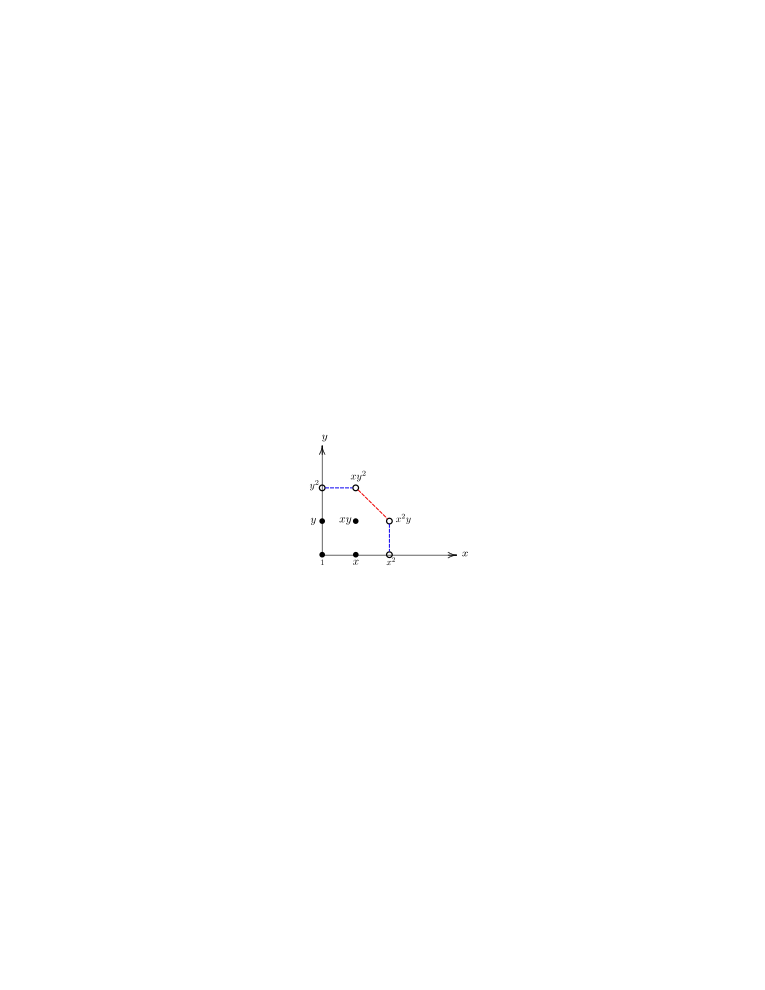
\includegraphics[width=0.5\linewidth]{Images/neighbors}
\caption{یکجمله‌ای‌های مرزی همسایه}
\label{fig:neighbors}
\end{figure}

\end{example}

\begin{definition}[\textbf{$S$-
		چندجمله‌ای}]
فرض کنید 
$G$
یک 
$\mO$-
پیش‌پایه‌ی مرزی باشد و 
$g_{i}, g_{j}\in G$،
به‌طوری که 
$g_{i} = b_{i} - \sum_{k}^{\mu}\alpha_{ki}t_{k}$
و
$g_{j} = b_{j} - \sum_{k}^{\mu}\alpha_{kj}t_{k}$.
در این‌صورت 
$S$-
چند جمله‌ای 
$g_{i}$
و
$g_{j}$
به‌صورت زیر تعریف می‌شود.
$$S_{ij} = (\frac{\lcm(b_{i},b_{j})}{b_{i}})*g_{i} - (\frac{\lcm(b_{i}, b_{j})}{b_{j}})*g_{j}.$$
\end{definition}

\begin{remark}
فرض کنید 
$G$
یک 
$\mO$-
پیش‌پایه‌ی مرزی باشد و 
$g_{i}, g_{j}\in G$
و 
$b_{i}$
و
$b_{j}$
همسایه باشند. 
\begin{enumerate}
\item
اگر  به ازای یک 
$x_{k}$
داشته باشیم 
$b_{j} = x_{k}b_{i}$
آن‌گاه 
$S_{ij} = g_{j} - x_{k}g_{i}$.
\item
اگر به ازای 
$x_{k}, x_{l}$
داشته باشیم، 
$x_{k}b_{i} = x_{l}b_{j}$
آن‌گاه 
$S_{ij} = x_{k}g_{i} - x_{l}g_{j}$.
\end{enumerate}
همان طور که مشاهده می‌شود، در هر دو حالت داریم 
$\Supp(S_{ij})\subseteq \mO\cup\po$.
 بنابراین 
 $a_{1},...,a_{\mu}\in K$
وجود دارند به‌طوری که
$$\nr_{\mO,G}(S_{ij}) = S_{ij} - \sum_{m = 1}^{\mu}a_{m}g_{m}\in I \ \wedge \ \Supp(\nr_{\mO,G}(S_{ij}))\subseteq \mO.$$
در این‌صورت اگر 
$G$
یک 
$\mO$-
پایه‌ی مرزی باشد، نتیجه می‌گیریم که 
$\nr_{\mO, G}(S_{ij}) = 0$.
\end{remark}

\begin{theorem}[\textbf{محک بوخبرگر برای پایه‌های مرزی}]
	\label{buchberger criterion for border basis}
فرض کنید 
$\mO = \orderideal$
یک ایده‌ال ترتیبی و 
$G = \prebasis$
یک 
$\mO$-
پیش‌پایه‌ی مرزی ایده‌ال 
$I$
باشد. در این‌صورت 
$G\subseteq I$
یک 
$\mO$-
پایه‌ی مرزی 
$I$
است اگر و تنها اگر یکی از شرط‌های معادل زیر برقرار باشد.
\begin{enumerate}
\item
به ازای هر 
$1\leq i\leq j\leq \nu$
،
داشته باشیم 
$S(g_{i}, g_{j})\xrightarrow{G}0$.
\item
به ازای هر 
$\{i,j\}$،
اگر 
$b_{i}$
و
$b_{j}$
همسایه باشند آن‌گاه 
$S(g_{i}, g_{j})\xrightarrow{G}0$
\item
به ازای هر 
$\{i, j\}$
اگر 
$b_{i}$
و
$b_{j}$
همسایه باشند آن‌گاه 
$\nr_{\mO, G}(S_{ij}) = 0$.
\item
به ازای هر 
$\{i, j\}$
،که 
$b_{i}$
و
$b_{j}$
همسایه هستند، ثابت‌های 
$c_{1},...,c_{\nu}\in K$
وجود دارند به‌طوری که
$$S(g_{i},g_{j}) = c_{1}g_{1} + \cdots + c_{\nu}g{\nu}.$$
\end{enumerate}
\end{theorem}
\begin{proof}
به 
{\small \cite[ص.۴۳۸]{cca2_kreuzer}}
، رجوع کنید.
\end{proof}

\subsection*{الگوریتم‌های محاسبه‌ی پایه‌ی مرزی}
این بخش از نظر ما مهمترین بخش مرتبط با پایه‌های مرزی است چرا که دلیل ترجیح ما در استفاده از پایه‌ی مرزی نسبت به پایه‌ی گروبنر در الگوریتم‌های محاسبه‌ی پایه‌ی مرزی نهفته است.

همان طور که قضیه‌ی 
\ref{gb bb relation th}
بیان می‌کند، پایه‌های مرزی تعمیمی از پایه‌های گروبنر برای ایده‌ال‌های صفربعدی هستند. در ابتدای این قسمت الگوریتمی تحت عنوان الگوریتم تغییر پایه را معرفی می‌کنیم، که با استفاده از محاسبه‌ی پایه‌ی گروبنر قادر است پایه‌ی مرزی را نیز محاسبه کند. نتیجه‌ی ضمنی این الگوریتم این است که محاسبه‌ی پایه‌ی مرزی نباید سخت‌تر از محاسبه‌ی پایه‌ی گروبنر باشد.
\begin{theorem}[\textbf{الگوریتم تغییر پایه}]
فرض کنید 
$I\subseteq P$
یک ایده‌ال چندجمله‌ای صفربعدی و 
$\mO$
یک ایده‌ال ترتیبی باشد. الگوریتم 
\ref{change basis alg}
با دریافت 
$\mO$
ابتدا مجاز بودن 
$\mO$
برای ایده‌ال 
$I$
را بررسی می‌کند، در صورتی که 
$\mO$
مجاز نباشد توقف کرده و مجاز نبودن 
$\mO$
را به عنوان خروجی تولید می‌کند در غیر این‌صورت، پس از متناهی مرحله اجرا، 
$\mO$-
پایه‌ی مرزی یکتای 
$I$
را محاسبه می‌کند.

\renewcommand{\algorithmicrequire}{\textbf{Input:}}
\renewcommand{\algorithmicensure}{\textbf{Output:}}
%\renewcommand{\algorithmicprint}{\textbf{break}}
\begin{algorithm}[H]
	\caption{الگوریتم تغییر پایه برای محاسبه‌ پایه‌ مرزی}
		\label{change basis alg}
	\begin{latin}
		\begin{algorithmic}[]		
			\REQUIRE  \rl{$\mO = \orderideal$
				و
				مولدی برای ایده‌ال $I$}
			\ENSURE $G = \prebasis$ 
			(\rl{$G$
				یک 
				$\mO$-
				پایه‌ی مرزی برای ایده‌ال 
				$I$
				است.})
			\STATE $\sigma\gets \text{\rl{یک ترتیب یکجمله‌ای}}$ 
			\STATE $\mO_{\sigma}(I)\gets \tn\backslash\lm_{\sigma}(I)$ 
			\IF{$|\mO_{\sigma}(I)| \neq \mu$}			
			\PRINT \rl{اندازه‌ی 
				$\mO$
				برای داشتن پایه‌ی مرزی کافی نیست}
			\RETURN
			\ENDIF
			\STATE $\{s_{1},...,s_{\mu}\}\gets \mO_{\sigma}(I)$			
			\FOR{$m\in\{1,...,\mu\}$}			
			\STATE $\sum_{i = 1}^{\mu}\tau_{im}s_{i}\gets \nf_{\sigma, I}(t_{m})$
			\ENDFOR
			\STATE $\mT\gets [\tau_{im}]_{1\leq i,m\leq \mu}$\rl					{ماتریسی که با 
				$\tau_{im}$
				ها پر شده.}	
			\IF{$\det(\mT) = 0$}					
			\PRINT \rl{$\mO$
				یک ایده‌ال ترتیبی پذیرفتنی نیست}			
			\RETURN
			\ENDIF
			\STATE $\border\gets \po$
			\FOR{$j\in \{1,...,\nu\}$}			
			\STATE $\sum_{i = 1}^{\mu}\beta_{ij}s_{i}\gets \nf_{\sigma, I}(b_{j})$			
			\ENDFOR
			\STATE $\mB\gets [\beta_{ij}]_{1\leq i\leq\mu, 1\leq j\leq \nu}.$		
			\STATE $[\alpha_{ij}]_{\mu\times\nu}\gets \mT^{-1}\mB$						
			\FOR{$j\in\{1,...,\nu\}$}			
			\STATE $g_{j}\gets\sum_{i=1}^{\mu}\alpha_{ij}t_{i}$	
			\ENDFOR		
			\RETURN $\{g_{1},...,g_{\nu}\}$
		\end{algorithmic}
	\end{latin}
\end{algorithm}

\end{theorem}
\begin{proof}
متناهی بودن مراحل اجرا بدیهی است و فقط صحت خروجی الگوریتم را ثابت می‌کنیم. طبق قضیه‌ی پایه‌ی مکالی 
\ref{macaulay basis th}،
$|\mO_{\sigma}(I)| = \dim_{\fld}(\frac{P}{I})$.
بنابراین وقتی شرط 
$|\mO|\neq|\mO_{\sigma}(I)|$
برقرار نیست الگوریتم با چاپ پیام «اندازه‌ی 
$\mO$
کافی نیست» خاتمه می‌یابد. همچنین طبق قضیه‌ی پایه‌ی مکالی کلاس‌های مانده اعضای 
$\mO_{\sigma}(I)$
یک پایه برای فضای برداری 
$\frac{P}{I}$
است. در گامی که 
$\nf_{\sigma,I}(t_{m})$
ها محاسبه می‌شوند، در واقع نمایش 
$\bar{t_{i}}$
ها نسبت به پایه‌ی 
$\overline{\mO}_{\sigma}(I) = \{\bar{s_{1}},...,\bar{s_{\mu}}\}$
برای 
$\frac{P}{I}$
به‌صورت زیر به‌دست  می‌آید:
$$\fa \ 1\leq i\leq \mu \ : \ \bar{t_{i}} = \tau_{1i}\bar{s_{1}} +\cdots+ \tau_{\mu i}\bar{s_{\mu}}$$
نمایش ماتریسی رابطه‌ی فوق به‌صورت 
$(\bar{t_{1}} \ \cdots \ \bar{t_{\mu}}) = (\bar{s_{1}} \ \cdots \ \bar{s_{\mu}})\mT$
است. بنابراین 
$\overline{\mO}$
یک پایه‌ برای فضای برداری 
$\frac{P}{I}$
است، اگر و تنها اگر 
$\mT$
معکوس‌پذیر باشد. از طرفی روابط زیر در $\frac{P}{I}$ برقرار است.

$$\bar{b_{j}} = (\bar{s_{1}} \ \cdots \ \bar{s_{\mu}})
\begin{pmatrix}
\beta_{1j}\\
\vdots\\
\beta_{\mu j}\\
\end{pmatrix}  = (\bar{t_{1}} \ \cdots \ \bar{t_{\mu}})\mT^{-1}\begin{pmatrix}
\beta_{1j}\\
\vdots\\
\beta_{\mu j}\\
\end{pmatrix}.$$
که نشان می‌دهد خروجی الگوریتم یک 
$\mO$
پایه‌ی مرزی برای 
$I$
است.
\end{proof}
الگوریتم فوق که توسط کروزِر و کِرین در سال ۲۰۰۶ در 
\cite{kehrein2006computing}
معرفی شد، شبیه الگوریتم شناخته‌ شده‌ی 
\lr{FGLM}
\cite{faugere1993efficient}
است، چرا که هر دو الگوریتم به ازای یک پایه‌ی گروبنر داده شده، با استفاده از تغییر پایه‌ی فضای برداری، پایه‌ای دیگر برای ایده‌ال محاسبه می‌کنند. با این‌حال بین الگوریتم تغییر پایه‌ و 
\lr{FGLM}
یک تفاوت اساسی وجود دارد، الگوریتم 
\lr{FGLM}
از پایه‌ی گروبنر داده شده تحت یک ترتیب یکجمله‌ای مثل 
$\sigma$
یکجمله‌ای‌های ایده‌ال ترتیبی 
$\mO_{\tau}$
نسبت به ترتیب یکجمله‌ای جدید 
$\tau$
را جمله به جمله محاسبه می‌کند، در حالی‌که الگوریتم تغییر پایه در فوق ایده‌ال ترتیبی 
$\mO$
را بطور کامل از ورودی دریافت می‌کند. 

الگوریتم تغییر پایه 
\ref{change basis alg}،
گرچه روشی سرراست برای محاسبه‌ی پایه‌ی مرزی تحت یک ایده‌ال ترتیبی پذیرفتنی، محسوب می‌شود ولی بدلیل محاسبه‌ی پایه‌ی گروبنر برای محاسبه‌ی فرم‌های نرمال و یا 
$\mO_{\sigma}(I)$
، تمام پیچیدگی‌های محاسبه‌ی پایه‌ی گروبنر را همراه دارد، که اصلاً مطلوب نیست، ضمن این‌که ایده‌ال ترتیبی به‌جای این‌که در الگوریتم محاسبه شود، یکی از ورودی‌ها است و ما تمایل داریم الگوریتمی طراحی کنیم که هم ایده‌ال ترتیبی و هم پایه‌ی مرزی متناظر با آن را محاسبه کند.

فرض کنید یک مجموعه‌ی مولد مثل 
$F = \{f_{1},...,f_{m}\}$
برای ایده‌ال صفربعدی
$I$
داده شده است، هدف ما این است که الگوریتمی داشته باشیم که با دریافت 
$F$
یک ایده‌ال ترتیبی پذیرفتنی برای 
$I$
مثل 
$\mO$
و یک 
$\mO$-
پایه‌ی مرزی برای 
$I$
 تولید کند. 
 
در سال ۱۹۹۹ مورِین
 الگوریتمی ارائه داد 
{\small \cite{mourrain1999new}}،
که قادر بود به ازای یک مولد داده شده از یک ایده‌ال صفر بعدی، پایه‌ای موسوم به پایه‌ی مورین که مفهومی کلی‌تر از پایه‌ی مرزی است را  برای ایده‌ال مورد نظر محاسبه کند. این الگوریتم برای محاسبه‌ی پایه‌ی مرزی طراحی نشده بود و خروجی آن لزوماً یک پایه‌ی مرزی نبود. هفت سال بعد از آن یعنی سال ۲۰۰۶، مارتین کِروزِر 
\LTRfootnote{Martin Kreuzer}
و آکِم کِرین
\LTRfootnote{Achim Kehrein}
با الهام گرفتن از الگوریتم مورِین، الگوریتمی برای محاسبه‌ی پایه‌ی مرزی  ایده‌ال های صفر بعدی ارائه دادند
{\small \cite{kehrein2006computing}}،
که در ادامه قصد داریم الگوریتم آن‌ها را مورد بررسی قرار دهیم.

\begin{definition}[\textbf{گسترش همسایگی}]
فرض کنید 
$P = \polyring$
و
$V\subseteq P$
یک زیر فضای برداری از 
$P$
باشد. 
\textit{گسترش همسایگی}
%\LTRfootnote{neighborhood extention}
$V$
را به‌صورت زیر تعریف می‌کنیم.
$$V^{+}:= V + x_{1}V + \cdots + x_{n}V.$$
واضح است که 
$V^{+}$
نیز یک فضای برداری در 
$P$
است. برای یک مجموعه‌ی متناهی از چندجمله‌ای‌ها نظیر 
$\mF = \{f_{1},...,f_{}\}$
نیز گسترش همسایگی، به‌صورت زیر تعریف می‌شود.
$$\mF^{+} := \mF\cup x_{1}\mF + \cup \cdots x_{n}\mF.$$
\end{definition}

\begin{remark}
فرض کنید 
$V\subseteq P = \polyring$
یک زیرفضای برداری و 
$\mF$
یک مجموعه از چندجمله‌ای‌ها باشد. اگر 
$\langle \mF\rangle_{\fld} = V$
آن‌گاه، 
$\langle \mF^{+}\rangle_{\fld} = \langle \mF \rangle_{\fld}^{+} = V^{+}$.
زیرا  عمل ضرب در یک متغیر نظیر 
$x_{i}$
در فضای برداری 
$P$،
یک تبدیل 
$\fld$-
خطی است.
در نتیجه برای گسترش همسایگی یک زیرفضای برداری مثل 
$V$
کافی است همسایگی یک مجموعه‌ی مولد 
$\fld$-
خطی آن را گسترش دهیم. 
\end{remark}

برای سادگی و فهم بهتر، ابتدا الگوریتم‌ اصلی را به الگوریتم‌های کوچکتر تبدیل می‌کنیم و پس از این‌که هر یک از الگوریتم‌های کوچکتر را شرح دادیم، در نهایت الگوریتم اصلی برای محاسبه‌ی پایه‌ی مرزی را شرح خواهیم داد. ولی قبل از آن بهتر است ایده‌ی اصلی و نقشه راه را بدانیم. هدف ما محاسبه‌ی پایه‌ی مرزی یک ایده‌ال صفر بعدی است، بنابراین اولین  گام یافتن یک ایده‌ال ترتیبی پذیرفتنی برای ایده‌ال مورد نظر است. به همین دلیل ابتدا الگوریتم‌هایی را معرفی می‌کنیم که به ازای یک مجموعه‌ی مولد داده شده برای ایده‌ال مورد نظر، قادرند یک ایده‌ال ترتیبی پذیرفتنی برای ایده‌ال تولید کنند. ایده‌ی 

\begin{definition}[\textbf{فضای برداری 
		$L$
		-پایا}]
فرض کنید 
$F\subseteq L$
زیرفضاهای برداری 
$P = \polyring$
باشند. در این‌صورت فضای برداری
$F$
را 
$L$
-پایا 
%\LTRfootnote{L-stabilized}
گویییم هرگاه 
$F^{+}\cap L = F$.
\end{definition}

\begin{definition}[\textbf{پوشش
		$L$-
		پایا}]
فرض کنید 
$F\subseteq L$
زیرفضاهای برداری 
$P$
باشند. پوشش 
$L$
-پایای 
$F$،
%\LTRfootnote{$L$-sateble span of F}،
عبارت است از کوچکترین فضای برداری شامل 
$F$
مثل 
$V$
به‌طوری که 
$V$
،
$L$-
پایا باشد، یعنی
$V^{+}\cap L = V$.
\end{definition}
گاهی اوقات یک فضای برداری 
$L$-
پایا را فضای برداری پایا نسبت به 
$L$
و  به همین ترتیب  پوشش 
$L$
-پایای یک فضای برداری را پوشش پایای آن فضا نسبت به فضای 
$L$
نیز  می‌گوییم.

\begin{example}
در زیر مثال‌هایی از فضاهای پایا نسبت به یک فضای برداری، آمده است.
\begin{enumerate}
\item
$L$
به ازای هر زیرفضای 
$P$
مثل 
$L$
، خود 
$L$
یک فضای برداری 
$L$-
پایا است. 
\item
فرض کنید 
$S = \{1, x, y, x^{2}y^{2}, y^{3}\}\subseteq P[x,y]$
و قرار دهید، 
$« = \langle S\rangle_{\fld}$.
در این‌صورت 
$\langle x + y, x^{2}, y^{2}, y^{3} \rangle_{\fld}$
یک فضای 
$L$
-پایا است ولی 
$\langle x + y, x^{2} \rangle_{\fld}$
چنین نیست. 
\end{enumerate}
\end{example}
 یک روش سرراست برای ساختن یک پوشش 
 $L$
 -پایا برای یک زیرفضای برداری نظیر 
 $F$
 به‌صورت زیر است:
 $$F_{0}: = F \ \wedge \ \fa k\in \mathbb{Z}_{\geq 0} :\ F_{k+1} = F_{k}^{+}\cap L$$
 در این صورت 
 $F_{L} = \bigcup_{k\geq 0}F_{K}$
 یک پوشش 
 $L$
 -پایا برای 
 $F$
 خواهد بود. در حالتی که 
 $\mF:= \{f_{1},...,f_{s}\}$
 یک مجموعه‌ی متناهی از چندجمله‌ای‌ها باشد، آن‌گاه 
 $F = \langle \mF\rangle_{\fld}$،
 $\fld$-
 فضای خطی تولید شده توسط 
 $\mF$
 است که یک زیرفضای 
 $P$
 است، در این حالت پوشش 
 $L$
 -پایای 
 $F$
 را با 
 $\mF_{L}$
 هم نمایش می‌دهیم. 
 
 در حالت خاصی که 
 $L = P$
 باشد آن‌گاه، پوشش 
 $L$
 -پایای 
 $\langle\mF\rangle_{\fld}$
همان ایده‌ال تولید شده توسط چندجمله‌ای‌های 
$\mF$
خواهد بود،  یعنی 
$F_{P} = \langle f_{1},...,f_{r}\rangle$.
البته ما برای محاسبات واقعی به همیشه 
$L$
را به‌جای یک زیرفضای 
$P$
با بعد متناهی در نظر می‌گیرم. در ادامه خواهید دید که الگوریتم‌های محاسبه‌ی پایه‌ی مرزی طوری طراحی‌ شده‌اند که تمام محاسبات در فضای با بعد متناهی 
$L$
انجام می‌شود و هیچ‌گاه عضوی خارج از فضای 
$L$
در محاسبات ظاهر نخواهد شد، به همین خاطر به 
$L$
فضای محاسباتی هم می‌گویند. در ادامه با برخی از ویژگی‌های اولیه‌ی پوشش‌های پایا آشنا خواهیم شد. 

\begin{lemma}
\label{propertice of l-stable span}
فرض کنید 
$F\subseteq G\subseteq \subseteq L$
زیرفضاهایی از فضای برداری 
$P = \polyring$
باشند. در این‌صورت داریم:
$$F\subseteq F_{L}, \  F_{L} = (F_{L})_{L}, \ F_{L}\subseteq G_{L}, \  F_{U}\subseteq F_{L}, \ F_{L} = (F_{U})_{L}.$$
\end{lemma}
\begin{proof}
به لم ۱۱ از 
{\small \cite{kehrein2006computing}}
، رجوع کنید.
\end{proof}
ویژگی آخر از لم 
\ref{propertice of l-stable span}
، یعنی 
$F_{L} = (F_{U})_{L}$
نشان می‌دهد که به‌جای محاسبه‌ی پوشش 
$U$-
پایا از همان ابتدا می‌توانیم  پوشش 
$L$
-پایا 
$F$
را محاسبه کنیم. 

یکی از مراحل الگوریتم اصلی برای محاسبه‌ی پایه‌ی مرزی، توسیع پایه‌ی یک فضای برداری است. فرض کنید 
$\mV$
پایه‌ی فضای بردای 
$\langle \mV \rangle_{\fld}\in P$ 
و 
$\mG$
مجموعه‌ای از چندجمله‌ای‌ها باشد و بخواهیم این پایه را به پایه‌ای برای فضای 
$\langle \mV \cup \mG\rangle_{K}$
گسترش دهیم، برای این‌کار می‌توانیم از الگوریتم حذف گاوس که جزئیات آن در لم بعد توضیح داده شده استفاده کنیم.
\begin{lemma}[\textbf{الگوریتم حذف گاوس در 
		$\fld$-
		فضای برداری 
		$\polyring$}]
	\label{gaussel lemma}
فرض کنید 
$\sigma$
یک ترتیب یکجمله‌ای و 
$\mV = \{v_{1},...,v_{r}\}\subseteq P\backslash\{0\}$
مجموعه‌ای متناهی از چندجمله‌ای‌های باشد به‌طوری که، ضریب پیشرو همه‌ی چندجمله‌ای‌های آن ۱ باشد و هر دو چندجمله‌ای از آن دارای یکجمله‌ای‌های پیشرو متمایز باشند. فرض کنید 
$\mG = \{g_{1},...,g_{s}\}\subseteq P$.
الگوریتم 
\hyperref[GaussEL]{\texttt{GaussEL}}
مجموعه‌ی 
$\mW\subseteq P$
را طوری محاسبه می‌کند که ضریب پیشرو همه‌ی چندجمله‌ای‌های آن ۱ است و هر دو چندجمله‌ای از 
$\mV\cup\mW$
دارای یکجمله‌ای پیشرو متمایز هستند و در ضمن 
$\langle \mV\cup \mW \rangle_{K} = \langle \mV\cup\mG \rangle_{K}$.
(مجموعه‌ی 
$\mV$
یا 
$\mW$
می‌تواند تهی باشد.)


\renewcommand{\algorithmicrequire}{\textbf{ورودی}}
\renewcommand{\algorithmicensure}{\textbf{خروجی}}
%\renewcommand{\algorithmicprint}{\textbf{break}}
\begin{algorithm}[H]
	\caption{الگوریتم حذف گاوس برای چندجمله‌ای‌ها-
		\lr{GaussEL}}
\label{GaussEL}	
	\begin{algorithmic}[1]				
		\REQUIRE $\mV$
		و
		$\mG$
		به صورتی که در لم شرح داده شده.
		\ENSURE $\mW$
		به‌صورتی که در لم شرح داده شده.
		\STATE قرار دهید 
		$\mH:=\mG$			
		و
		$\eta:= 0$
		\STATE اگر 
		$\mH = \emptyset$			
		آن‌گاه 
		$\mW:=\{v_{r + 1},...,v_{r + \eta}\}$
		و الگوریتم متوقف می‌شود.
		\STATE $f\in \mH$			
		را انتخاب کرده و آن را از 
		$\mH$
		حذف می‌کنیم و قرار می‌دهیم 
		$i:=1$.
		\STATE اگر 
		$f = 0$
		یا 
		$i > r + \eta$
		آن‌گاه به گام ۷ می‌رویم.
		\STATE اگر
		$\lm_{\sigma}(f) = \lm_{\sigma}(v_{i})$			
		آن‌گاه 
		$f$
		را با 
		$f - \lm_{\sigma}(f)*v_{i}$
		جایگزین کرده و قرار می‌دهیم، 
		$i := 1$
		و به گام ۴ می‌رویم.
		\STATE مقدار 
		$i$					
		را یک‌واحد افزایش داده و به گام ۴ می‌رویم.
		\STATE اگر 
		$f\neq 0$
		آن‌گاه 
		$\eta$
		را یک‌واحد افزایش داده  و قرار می‌دهیم 
		$v_{r + \eta}:=\frac{f}{\lm_{\sigma}(f)}$
		و با گام ۲ ادامه می‌دهیم.						
	\end{algorithmic}
\end{algorithm}
\end{lemma}
\begin{proof}
به لم ۱۲ 
{\small \cite{kehrein2006computing}}
، رجوع کنید.
\end{proof}

دلیل این‌که در الگوریتم 
\hyperref[GaussEL]{\texttt{GaussEL}}
شرط کردیم که اعضای پایه‌ی 
$\mV$
دوبه‌دو دارای یکجمله‌ای پیشرو متمایز باشند این است که اگر 
$\mV = \{v_{1},...,v_{r}\}$
پایه‌ای برای زیرفضای 
$V\subseteq P$
با خصوصیت ذکر شده باشد، آن‌گاه 
$\lm_{\sigma}(V):=\{\lm_{\sigma}(v)| \ v\in
 V\backslash\{0\}\}$
 با 
 $\lm_{\sigma}(\mV):= \{\lm_{\sigma}(v_{1}),...,\lm_{\sigma}(v_{r})\}$
 برابر خواهد شد. 
 
 \begin{definition}[\textbf{ترتیب یکجمله‌ای سازگار با درجه}]
ترتیب یکجمله‌ای
$\sigma$
روی 
$\tn$
را
\textit{سازگار با درجه}
گوییم هرگاه به ازای هر 
$t_{1},t_{2}\in\tn$
، اگر 
$t_{1}\geq_{\sigma} t_{2}$
آن‌گاه 
$\deg(t_{1})\geq \deg(t_{2})$.
 \end{definition}
 برای مثال ترتیب الفبایی مدرج و الفبایی مدرج معکوس ترتیب‌های یکجمله‌ای سازگار با درجه هستند.
 
 با استفاده از الگوریتم 
 \hyperref[GaussEL]{\texttt{GaussEL}}،
 در گزاره‌ی بعدی الگوریتمی برای محاسبه‌ی پوشش 
 $L$
 -پایای یک فضای برداری وقتی 
 $L = \langle \tnd \rangle_{K}$
 است ارائه می‌کنیم. 
 
\begin{proposition}[\textbf{محاسبه‌ی پوشش پایا}]
\label{stable span coputation}
فرض کنید 
$\mF := \{f_{1},...,f_{r}\}\subseteq P$
و
$L:=\langle \tnd \rangle_{\fld}$
به‌طوری که 
$f_{1},...,f_{r}\in L$
، یعنی داشته باشیم 
$d\geq \max\{\deg(f_{i})| \ 1\leq i\leq r\}$.
فرض کنید 
$\sigma$
یک ترتیب یکجمله‌ای سازگار با درجه باشد، در این‌صورت الگوریتم 
\ref{computing stable span alg}
پایه‌ی پوشش 
$L$
پایای 
$\mF$
یعنی پایه‌ی 
$\mF_{L}$
را محاسبه‌ می‌کند. علاوه بر این چندجمله‌ای‌های پایه‌ی محاسبه شده دارای یکجمله‌ای‌های پیشرو متمایز هستند. 

\renewcommand{\algorithmicrequire}{\textbf{Input}}
\renewcommand{\algorithmicensure}{\textbf{Output}}
%\renewcommand{\algorithmicprint}{\textbf{break}}
\begin{algorithm}[]
	\caption{الگوریتم محاسبه‌ی پوشش پایای یک فضای برداری}
	\label{computing stable span alg}
	\begin{latin}	
	\begin{algorithmic}[]				
		\REQUIRE $\mF = \{f_{1},...,f_{r}\}, \ L = \langle \tnd \rangle_{K}$
		با ویژگی‌های ذکر شده در لم.
		\ENSURE \rl{$\mV$
			که پایه‌ای برای فضای برداری 
			$\mF_{L}$
			است}
\STATE $\mV\gets \hyperref[GaussEL]{GaussEL}(\emptyset, \mF)$		
\REPEAT 
\STATE $\mW'\gets \hyperref[GaussEL]{GaussEL}(\mV, \mV^{+}\backslash \mV)$
\STATE $\mW\gets  \{w\in\mW'| \ \deg(w)\leq d\} = \{w\in\mW'| \ \Supp(w)\subseteq L\}$
\UNTIL{$\mW \neq \emptyset$}
\RETURN $\mV$		
\end{algorithmic}
\end{latin}
\end{algorithm}

\end{proposition}
\begin{proof}
به گزاره‌ی ۱۳ در 
{\small \cite{kehrein2006computing}}
، مراجعه کنید. 
\end{proof}

\begin{corollary}
طبق تعریف، پوشش 
$L$
-پایای 
$\mF$
یعنی 
$\mF_{L}$
مشمول در فضای برداری 
$L$
است. از طرفی بدیهی است که 
$\mF_{L}$
مشمول در ایده‌ال تولید شده به‌وسیله‌ی 
$\mF$
نیز قرار دارد  در نتیجه 
$\mF_{L}\subseteq L\cap \langle \mF \rangle$.
\end{corollary}

\begin{example}
فرض کنید 
$\mF = \{f_{1}, f_{2}, f_{3}\}$
که 
$f_{1} = x^{2}y^{2} + 1, f_{2} = x^{4}$
و
$f_{3} = y^{4}$.
همچنین فرض کنید 
$\mH = \{1\}$.
هر دو مجموعه‌ ایده‌ال 
$\langle 1\rangle$
را تولید می‌کنند زیرا 
$1 = f_{2}*f_{3} - f_{1}^{2} + 2f_{1}$.

\begin{enumerate}
\item
فرض کنید 
$L = \langle \tn_{\leq 4}\rangle_{\fld}$.
در این‌صورت 
$\mF_{L} = \langle \mF\rangle$
و
$\dim_{\fld}(\mF_{L}) = 3$،
در حالی که 
$\mH = L$
و 
$\dim_{\fld}(\mH_{L}) = 10$.
\item
اگر 
$L = \langle \tn_{\leq 5}\rangle_{\fld}$،
آن‌گاه 
$\mF_{L} = L = \mH_{L}$.
\end{enumerate}
\end{example}

اولین هدف ما یافتن یک ایده‌ال ترتیبی پذیرفتنی برای ایده‌ال داده شده است و گزاره‌ی بعدی نشان می‌دهد که پوشش پایایی که در الگوریتم 
\ref{computing stable span alg}
محاسبه می‌شود، حاوی اطاعاتی در مورد کاندید‌های ایده‌ال ترتیبی پذیرفتنی برای ایده‌ال تولید شده توسط چندجمله‌ای‌های  مجموعه‌ی 
$\mF$
است.

\begin{proposition}
فرض کنید 
$\mF = \{f_{1},...,f_{s}\}\subseteq P$
و
$L = \langle \tnd \rangle_{\fld}$
به‌طوری که 
$\mF\subseteq L$.
در این‌صورت یک ایده‌ال ترتیبی مثل 
$\mO$
وجود دارد به‌طوری که،
$$L = \mF_{L}\oplus \langle \mO \rangle_{\fld}$$.
یعنی، اگر 
$\sigma$
یک ترتیب یکجمله‌ای سازگار با درجه  و 
$\mV = \{v_{1},...,v_{r}\}$
پایه‌ی محاسبه شده برای 
$\mF_{L}$
توسط الگوریتم 
\ref{computing stable span alg}
باشد، آن‌گاه چندجمله‌ای‌های 
$\mV$
دوبه‌دو دارای یکجمله‌ای‌های پیشرو متمایز بوده و 
$\lm_{\sigma}(\mF_{L})$
تحت مضارب اعضای خود در 
$L$
بسته است. یعنی اگر به ازای یک 
$v\in \mF_{L}$
و یک یکجمله‌ای 
$t\in \tnd$
داشته باشیم، 
$\lm_{\sigma}(v)\mid t$
، آن‌گاه یک 
$w\in \mF_{L}$
وجود دارد به‌طوری که 
$t = \lm_{\sigma}(w)$.
بطور معادل 
$\mO = \tnd\backslash \{\lm_{\sigma}(v_{1}),...,\lm_{\sigma}(v_{r})\}$
یک ایده‌ال ترتیبی است که در رابطه‌ی جمع مستقیم فوق نیز صدق می‌کند. 
\end{proposition}
\begin{proof}
به گزاره‌ی ۱۵ 
{\small \cite{kehrein2006computing}}
، مراجعه کنید.
\end{proof}

گزاره‌ی بعدی به عنوان شرط توقف در الگوریتم محاسبه‌ی پایه‌ی مرزی که در ادامه ارائه می‌کنیم به‌کار خواهد رفت. در واقع توسط گزاره‌ی بعدی می‌توان پی‌برد که کدام‌یک از کاندید‌های به‌دست  آمده برای ایده‌ال ترتیبی ، می‌توانند ایده‌ال ترتیبی پذیرفتنی برای ایده‌ال داده شده باشند.

\begin{proposition}
	\label{stop criterion}
	فرض کنید 
	$L$
	یک زیرفضای برداری 
	$P$
	و 
	$\tilde{I}$
 یک زیرفضای برداری ایده‌ال صفر بعدی 
	$I\subseteq P$
	باشد، به‌طوری که 
	$\tilde{I}^{+}\cap L = \tilde{I}$
	و
	$\langle \tilde{I} \rangle = I$
	، به‌عبارت دیگر 
	$\tilde{I}$
	یک فضای 
	$L$-
	پایا باشد که ایده‌ال تولید شده توسط آن برابر 
	$I$
است. علاوه بر این فرض کنید 
$\mO$-
یک ایده‌ال ترتیبی باشد که در رابطه‌ی 
$L = \tilde{I}\oplus \langle \mO\rangle_{\fld},$
صدق می‌کند. در این‌صورت اگر 
$\po\subseteq L$
آن‌گاه 
$\mO$
یک ایده‌ال ترتیبی پذیرفتنی برای 
$I$
خواهد بود.
\end{proposition}
\begin{proof}
به ازای هر یکجمله‌ای مرزی 
$b_{j}\in\po\subseteq L$
بر اساس  رابطه‌ی جمع مستقیم فوق، چندجمله‌ای 
$g_{j}\in \tilde{I}$
وجود دارد به‌طوری که 
$$b_{j} = g_{j} + \sum_{i = 1}^{m}\alpha_{ij}t_{i}\in\tilde{I}\oplus \langle\mO\rangle_{\fld}.$$
به این ترتیب می‌توان مجموعه‌ی 
$G = \{g_{1},...,g_{\nu	}\}$
را به‌دست  آورد که یک 
$\mO$-
پیش‌پایه‌ی مرزی است.

فرض کنید 
$g_{k}$
و
$g_{l}$
دو همسایه‌ی دلخواه از پیش‌پایه‌ی 
$G$
باشند. در این‌صورت یکجمله‌ای‌های 
$S$-
چندجمله‌ای‌ آن‌ها یعنی 
$S(g_{k}, g_{l})\in\tilde{I}^{+}$
در 
$\mO^{+}$
قرار می‌گیرند. بنابراین ضرایب 
$c_{j}\in\fld$
وجود دارند به‌طوری که، یکجمله‌ای‌های عبارت 
$h:= S(g_{k},g_{l}) - \sum_{j = 1}^{\nu}c_{j}g_{j}$
در 
$\mO$
قرار می‌گیرند. در نتیجه 
$h\in \tilde{I}^{+}\cap\langle \mO\rangle_{K} = \tilde{I}^{+}\cap L\cap\langle \mO\rangle_{\fld} = \{0\}$.
در نهایت طبق محک بوخبرگر برای پایه‌ی مرزی
\ref{buchberger criterion for border basis}
، 
$G$
یک 
$\mO$-
پایه‌ی مرزی خواهد بود.
\end{proof}
دقت کنید، اگر در قضیه‌ی فوق جای به‌جای 
$\tilde{I}$،
ایده‌ال 
$I$
و به‌جای 
$L$
کل فضای 
$P$
را قرار دهیم، به تعریف پایه‌ی مرزی خواهیم رسید.

یک جمع بندی از مباحث قبل نشان می‌دهد که می‌توانیم در ابتدا با استفاده از الگوریتم 
\ref{computing stable span alg}
پوشش پایای فضای 
$\fld$-
خطی تولید شده توسط مجموعه‌ی مولد داده شده را  نسبت به یک فضای برداری مثل 
$\langle\tnd \rangle_{\fld}$
به‌دست  آوریم. سپس این مجموعه کاندید‌هایی را برای ایده‌ال ترتیبی پذیرفتنی معرفی می‌کند که با استفاده از گزاره‌ی 
\ref{stop criterion}
می‌توانیم، کاندیدی که یک ایده‌ال ترتیبی پذیرفتنی است تشخیص دهیم. بعد از این مراحل یک ایده‌ال ترتیبی پذیرفتنی به‌دست  می‌آید و به یک الگوریتم نیاز داریم که پایه‌ی مرزی ایده‌ال نسبت به ایده‌ال ترتیبی به‌دست  آمده را استخراج کند. این الگوریتم در گزاره‌ی بعدی ارائه شده است.

\begin{proposition}
\label{final reduction th}
فرض کنید 
$\mF = \{f_{1},...,f_{s}\}\subseteq P$
یک مجموعه‌ي مولد داده شده برای ایده‌ال صفربعدی 
$I$
باشد. فرض کنید 
$\sigma$
یک ترتیب یکجمله‌ای سازگار با درجه و 
$L$
یک ایده‌ال ترتیبی (برای مثال 
$L = \tnd$)
باشد. در ضمن فرض کنید 
$\mV$
یک پایه‌ برای پوشش 
$L$
پایای 
$\mF$
یعنی فضای برداری
$\mF_{L}$
باشد که یکجمله‌ای‌های پیشرو هر دو عضو آن متمایز باشند و 
$\mO = L\backslash \lm_{\sigma}(\mV)$
به‌طوری که
$$L = \mF_{L}\oplus \langle \mO\rangle_{\fld} \ \wedge \ \po\subseteq L.$$
در این‌صورت الگوریتم 
\ref{final reduction alg}، 
$\mO_{\sigma}(I)$-
پایه‌ی مرزی 
$I$
را محاسبه می‌کند. 
\begin{algorithm}[]
	\renewcommand{\algorithmicrequire}{\textbf{ورودی}}
	\renewcommand{\algorithmicensure}{\textbf{خروجی}}
	\caption{الگوریتم تحویل نهایی- \lr{Final Reduction}}
	\label{final reduction alg}
	\begin{algorithmic}[1]		
		\REQUIRE $\mF, L$
		و
		$\sigma$
		و
		$\mO, \mV$
		با ویژگی‌های ذکر شده در لم.
		
		\ENSURE $\mO_{\sigma}(I)$
		-پایه‌ی مرزی 
		$I$.
		\STATE $\mV_{R} = \emptyset$
		\STATE اگر 
		$\mV = \emptyset$
		آن‌گاه به گام ۸ می‌رویم.
		\STATE عضو 
		$v\in \mV$
		را برابر با عضوی از 
		$\mV$
		 که دارای یکجمله‌ای پیشرو مینیمال است قرار داده و آن‌را از 
		 $\mV$
		 حذف می‌کنیم.
		 \STATE $\mH:= \Supp(v)\backslash (\{\lm_{\sigma}(v)\}\cup \mO)$		 
		 \STATE اگر 
		 $\mH = \emptyset$
		 آن‌گاه 
		 $\frac{v}{\lc_{\sigma}(v)}$
		 را به 
		 $\mV_{R}$
		 ضمیمه کرده و به گام ۲ می‌رویم.
		 \STATE برای هر 
		 $h\in\mH$
		 ، 
		 $w_{h}\in \mV_{R}$
		 و
		 $c_{h}\in K$
		 را طوری محاسبه می‌کنیم که 
		 $\lm_{\sigma}(w_{h}) = h$
		 و\\
		 {\small $h\notin \Supp(v - c_{h}*w_{h})$}.
		 \STATE $v$		 
		 را با مقدار جدید 
		 $v - \sum_{h}c_{h}*w_{h}$
		 جایگزین کرده و 
		 $\frac{v}{\lc_{\sigma}(v)}$
		 را به 
		 $\mV_{R}$
		 ضمیمه می‌کنیم، سپس به گام ۲ می‌رویم.
		 \STATE فرض کنید 
		 $\po = \{b_{1},...,b_{\nu}\}$.
		 به ازای هر 
		 $b_{j}\in\po$
		 چندجمله‌ای 
		 $g_{j}\in\mV_{R}$
		 را طوری انتخاب می‌کنیم که 
		 $b_{j} = \lm_{\sigma}(g_{j})$
		،در این‌صورت، خروجی عبارت‌است از 
		 $g_{1},...,g_{\nu}$.
	\end{algorithmic}
\end{algorithm}
\end{proposition}
\begin{proof}
به گزاره‌ی ۱۷ از 
{\small \cite{kehrein2006computing}}
، مراجعه کنید.
\end{proof}

اکنون با کنار هم قرار دادن الگوریتم‌های قبلی الگوریتمی برای محاسبه‌ی پایه‌ی مرزی یک ایده‌ال صفر بعدی به ازای یک مولد داده شده، ارائه می‌دهیم.

\begin{proposition}[\textbf{الگوریم محاسبه‌ی پایه‌ی مرزی}]
فرض کنید 
$\mF = \{f_{1},...,f_{s}\}\subseteq P$
مولدی برای ایده‌ال صفربعدی 
$I = \langle\mF\rangle$
باشد. فرض کنید 
$\sigma$
یک ترتیب یکجمله‌ای سازگار با درجه باشد. در این‌صورت الگوریتم 
\ref{BBA}، 
$\mO_{\sigma}(I)$
-پایه‌ی مرزی 
$I$
را محاسبه می‌کند.
\begin{algorithm}[t]
	\renewcommand{\algorithmicrequire}{\textbf{ورودی}}
	\renewcommand{\algorithmicensure}{\textbf{خروجی}}
	\caption{الگوریتم محاسبه‌ی پایه‌ مرزی-\lr{BBA}}
	\label{BBA}	
	\begin{algorithmic}[1]		
		\REQUIRE $\mF, \sigma$
		آن‌گونه که در لم گفته شده.
		\ENSURE $\mO_{\sigma}(I)$
		-پایه‌ی مرزی برای 
		$I$.
		\STATE $d:=\max\{\deg(f_{i})| \ 1\leq i\leq s\}, \ L:= \langle \tnd\rangle_{\fld}$
		\STATE پایه‌ی 
		$\mV = \{v_{1},...,v_{r}\}$		
		را برای 
		$\langle \mF\rangle_{\fld}$
		محاسبه می‌کنیم طوری که یکجمله‌ای‌های پیشرو اعضایش متمایز باشند.
		\STATE پایه‌ی توسیع یافته 
		$\mW' := \{v'_{r + 1},...,v'_{r+\eta'}\}$
		برای 
		$\langle\mV^{+}\rangle_{\fld}\supseteq\langle \mV\rangle_{\fld}$
		را طوری محاسبه می‌کنیم که یکجمله‌ای‌های پیشرو اعضای 
		$\mV\cup\mW'$
		متمایز باشند.
		\STATE $\mW = \{v_{r+1},...,v_{r+\eta}\} = \{v\in\mW'| \ \deg(v)\leq d\}.$
		\STATE اگر 
		$\eta >0$
		آن‌گاه 
		$\mV$
		را با 
		$\mV\cup \mW$
		جایگزین کرده، قرار می‌دهیم 
		$r = r + \eta$
		و سپس به گام ۳ می‌رویم. 
		\STATE $\mO: = \tnd \backslash \{\lm_{\sigma}(v_{1}),...,\lm_{\sigma}(v_{r})\}$.
		\STATE اگر 
		$\po \nsubseteq	L$
		، 
		$d$
		را یک‌واحد افزایش داده و قرار می‌دهیم 
		$L:=\langle\tnd\rangle_{\fld}$ 
		و  سپس به گام ۳ می‌رویم. 
		\STATE با فراخوانی  الگوریتم تحویل نهایی
		[\ref{final reduction alg}]							
چندجمله‌ای‌های 
$g_{1},...,g_{\nu}$
را که این الگوریتم محاسبه می‌کند به عنوان خروجی نهایی الگوریتم در نظر می‌گیریم.
	\end{algorithmic}
\end{algorithm}
\end{proposition}
\begin{proof}
رجوع کنید به 
\cite{cca2_kreuzer}.
\end{proof}
این بحث را در این‌جا خاتمه می‌دهیم. در فصل ۴ که روش‌های حل دستگاه چندجمله‌ای را معرفی می‌کنیم، الگوریتمی بهینه‌تر برای محاسبه‌ی پایه‌ی مرزی ارائه می‌دهیم که برای حل دستگاه‌های به‌دست آمده از سامانه‌های رمزنگاری مناسب‌تر است. 



